\documentclass[11pt,a4paper,english,oneside]{book}
\usepackage{etex} %Because of many packages --> Extended TeX.
\usepackage[left=1in, right=1in]{geometry} %Helps to structure the paper layout.
\usepackage[Lenny]{fncychap} %Design of the thesis.
\usepackage[utf8]{inputenc} %Due to vowels.
\usepackage{babel} %Define the language style.
\usepackage{dsfont} %Nice style for the indicator function.
\usepackage{fancyhdr} %To customize the headers and footers.
\usepackage{booktabs} %In case you need \cmidrule or \addlinespace in tables.
\usepackage[hang,bottom,stable,multiple]{footmisc} %Style of footnotes.
\usepackage{appendix} %For the \appendixpage command.
%Load some mathematical packages.
\usepackage{amsmath}
\usepackage{amsfonts}
\usepackage{amsmath}
\usepackage{amssymb}
\usepackage{mathtools}
%\usepackage[sort,round]{natbib} %For the bibliography.
\usepackage[natbibapa]{apacite} %for citing and bibliography, by Corinne
\usepackage{etoolbox} %To remove the page number on \appendixpage.
\usepackage{amsthm} %For theorems, definitions etc.
\usepackage{thmtools} %For theorems, definitions etc.
\usepackage{setspace} %Use double spacing.
\usepackage{lipsum} %For the \lipsum command to generate a text.
\usepackage{datetime} %For the specification of the date.
%\usepackage{tocloft} %The ToC, LoF and LoT each appear not necessarily on a new page.
\usepackage{graphicx,listings, xcolor, colortbl, textcomp} %For the graphics, listings etc.
\usepackage{mcode} %To implement a Matlab code.
\usepackage[margin=10pt, font=small, labelfont=bf, labelsep=endash]{caption} %Customize the captions.
\usepackage{chngcntr} %To use counterwithout.
\usepackage{epstopdf} %For inserting .eps files into the document.
\usepackage{hyperref} %Must be loaded at the end.
\usepackage{xparse} %Load for \NewDocumentCommand command.
\usepackage{cleveref} %For the command \cref, load after hyperref.
\usepackage{arydshln} %Due to the capability to draw horizontal/vertical dash-lines.
\usepackage{array,hhline} %To create tables and matrices.
\usepackage{rotating} %To rotate a table.
\usepackage{tabularx} %An extended version of tabular.
\usepackage{makecell}
\usepackage{booktabs}
\newcommand{\tabitem}{~~\llap{\textbullet}~~}

%Setup of the reference links.
\hypersetup{
     colorlinks=false,
     linkcolor=blue,
     citecolor=blue,
     filecolor=magenta,
     urlcolor=blue}

%Define some reasonable margins.
%\setlength{\textwidth}{6.6in}
\setlength{\textheight}{9.3in}
\setlength{\topmargin}{-0.1in}
%\setlength{\oddsidemargin}{0in}
\setlength{\parskip}{1mm}

\bibliographystyle{apacite} %Reference style.
\allowdisplaybreaks[1] %Page breaks of equations are allowed, but avoided if possible. 2-4 more relaxed.

%New command for the logo.
\newcommand*{\plogo}{
\includegraphics[scale=0.7]{Images/HSG_logo}}

%New command for the differential d to have an ordinary d.
\makeatletter
  \newcommand{\ud}{\mathrm{d}}
\makeatother

%Remove page number on \appendixpage. Use the package 'etoolbox'.
\makeatletter
\patchcmd{\@chap@pppage}{\thispagestyle{plain}}{\thispagestyle{empty}}{}{}
\makeatother

%Declare Definitions, Theorems etc.
%%%%%%%%%%%%%%%%%%%%%%%%%%%%%%%%%%%%%%%%%%%%%%%%%%%%%%%%%%%%%%%%%%%%%%%%%%%%%%%%%%%%%%%%%%%%%%%%%%%%%%%%%%%%%%%%%%%
\declaretheorem[style=definition,qed=$\blacktriangleleft$, numberwithin=chapter]{remark} %additional options; numberwithin=,..., see 'Thmtools' Users’ Guide
\declaretheorem[style=definition,qed=$\triangle$,numberwithin=chapter]{definition}
\newtheorem{ass}{Assumption}[chapter]
\newtheorem{prop}{Proposition}[chapter]
\newtheorem{lemma}{Lemma}[chapter]
\declaretheorem[style=definition,qed=$\perp$,numberwithin=chapter]{example}
\newtheorem{theorem}{Theorem}[chapter]
\newtheorem{coroll}{Corollary}[chapter]
%%%%%%%%%%%%%%%%%%%%%%%%%%%%%%%%%%%%%%%%%%%%%%%%%%%%%%%%%%%%%%%%%%%%%%%%%%%%%%%%%%%%%%%%%%%%%%%%%%%%%%%%%%%%%%%%%%%
\definecolor{forestgreen}{rgb}{100,100,100} 
\definecolor{forestgreen}{rgb}{0,255,0} 
\definecolor{darkgreen}{rgb}{0,75,50}
%%%%%%%%%%%%%%%%%%%%%%%%%%%%%%%%%%%%%%%%%%%%%%%%%%%%%%%%%%%%%%%%%%%%%%%%%%%%%%%%%%%%%%%%%%%%%%%%%%%%%%%%%%%%%%%%%%%

%\clubpenalty = 10000 %von Corinne
%\widowpenalty = 10000
%\displaywidowpenalty = 10000


%Readjust the numbering.
%\counterwithout{footnote}{chapter}
\numberwithin{equation}{chapter}

%\setlength{\parindent}{0cm} %Uncomment this if you don't want to have indents.

%----------------------------------------------------------------------------------------
%	TITLE PAGE
%----------------------------------------------------------------------------------------
\newcommand*{\titleGP}{\begingroup %Create the command for including the title page in the document.
\centering %Center all text.
\vspace*{\baselineskip} %White space at the top of the page.
\plogo\\[2\baselineskip] %University Logo.
\rule{\textwidth}{1.6pt}\vspace*{-\baselineskip}\vspace*{2pt} %Thick horizontal line.
\rule{\textwidth}{0.4pt}\\[\baselineskip] %Thin horizontal line.
{\LARGE Narratives in Finance }\\[0.2\baselineskip] %Title.
\rule{\textwidth}{0.4pt}\vspace*{-\baselineskip}\vspace{3.2pt} %Thin horizontal line.
\rule{\textwidth}{1.6pt}\\[2\baselineskip] %Thick horizontal line.
\scshape %Small caps.
Master's Thesis\\[2\baselineskip]
Submitted in partial fulfillment of the requirements for the degree of Master of Arts in Quantiative Economics and Finance \par
\vspace*{2\baselineskip}
Author\\
{\Large Corinne Knöpfel \\ [5pt]
 }
Wiesen 2488, Herisau \\[5pt]
11-613-676\\[5pt]
corinne.knoepfel@student.unisg.ch \\


\vspace*{2\baselineskip}
Supervisor\\
{\Large Dr. Peter Gruber\\[5pt]%\small Hans Vontobel Professor of Financial Engineering\\[5pt]
\small Institute of Finance\\[5pt]Universit\`{a} della Svizzera Italiana\par}
%\vspace*{2\baselineskip}
%Assistant\\
%{\Large [ Name ] \par}
\vfill
{\scshape %Date of Submission: 
	\today } \\[0.3\baselineskip]
\endgroup}

%Special header and footer style for the Abstract and other special pages.
\fancypagestyle{firststyle}{%
  \fancyhf{}%
  \renewcommand{\headrulewidth}{0pt}
  \fancyfoot[C]{\thepage}
}


%Customize headers and footers.
\pagestyle{fancy}
\fancyhead[R]{\thepage}
\fancyhead[L]{\rightmark} %section in header
%\fancyhead[L]{\leftmark}  %chapter in header
%\fancyfoot[L]{[ Your Name ]}
\fancyfoot[C]{}
%\fancyfoot[R]{[ Running Master Thesis Title ]}

%Define the signature line with dots.
\NewDocumentCommand \dotbox {o O{.5\linewidth} m O{3ex} O{\linewidth}}
{
  \begin{minipage}{7cm}
    \makebox[7cm][l]{\,.\dotfill}
    \\
    \makebox[7cm][l]{\,#3}
  \end{minipage}
}

\begin{document}
\thispagestyle{empty}
\titleGP
\newpage
\doublespacing
\setcounter{page}{1}
\pagenumbering{Roman}
%\section*{Task Assignment}
\thispagestyle{firststyle}
%\pagestyle{firststyle} %from here on it uses pagestyle firststyle (for content, etc.)


%\newpage
\chapter*{Abstract}

{\pagestyle{firststyle}
\tableofcontents
\cleardoublepage
}

\listoffigures
\listoftables
%\setcounter{rememberpage}{\value{page}} %in case we want to go back to Roman numbering in the Appendix

\newpage


\pagenumbering{arabic}
% \part{[ Part title ]}
\chapter{Introduction}
 

\chapter{Monetary Policy and Interest Rates} \label{MonetaryPolicy}
 
\noindent However little understood, the relationship between monetary policy and market interest rates is undeniable. Interest rates of all maturities react to changes in monetary policy, creating opportunities and risks for traders, challenges for policy makers, and puzzling effects for academics to study \citep[p. 1594]{Ellingsen.2001}. 

Target rate changes in particular have an impact on the bond market and on interest rates \citep[p. 332]{Cook.1989}. %Overall, there is an invested interest in how monetary policy impacts yield curve movement.
Yet, the understanding of yield curve movements is incomplete at best. On average, the relationship between monetary policy and interest rates appears to be positive: An increase in the central bank's target rate leads to an increase in the interest rates of all maturities. However, there are many instances where this simple rule has proven false and interest rates of long maturities fell in response to an increase in the central bank's rate \citep[p. 1594]{Ellingsen.2001}. 

Chapter \ref{SensitivityPuzzle} gives an account of the puzzle posed by the inconsistent response of long-term rates, Chapter \ref{ExistingResearch} touches on previous research and possible explanations, and Chapter  \ref{NewInsights} outlines how an investigation of narratives might be able to shed light on this puzzle.


\section{Excess Sensitivity Puzzle} \label{SensitivityPuzzle}

\cite{Cook.1989} analyzed financial data from the late 70s and found that the U.S. Federal Reserve (Fed), by setting the target for the federal funds rate, had a strong influence on interest rate movements. While short-term rates reacted particularly strongly, changes in the target rate also caused small but significant movements in long-term rates. 
 
It is not surprising that short-term rates follow the target rate closely, after all the Fed keeps the overnight rate close to the target and thus directly influences the one-month rate \citep[p. 1]{Ellingsen.2003}. The movements of the long-term rates are more ambiguous. \citet[pp. 343--346]{Cook.1989} interpret the fact that, on average, 10-year and 30-year bonds co-move with the short-term rates as evidence for the expectation theory of the term structure of interest rates. According to the expectation theory, long-term rates are equal to short-term rates over the same period of time plus a term premium. Thus, an increase in the short-term rates is expected to drive up long-term rates as well, but to a lesser extent \citep[p. 1594]{Ellingsen.2001}.

To \cite{Romer.2000}, on the other hand, the response of long-term rates presents a puzzle. They argue that standard theory predicts a drop in inflation as short-term rates rise, which ought to lead to a reduction in long-term rates. The opposite can be observed, however: Interest rates for all maturities typically rise following an increase in the target rate. \cite{Romer.2000} explain this anomaly with information-asymmetry between the Fed and the general public. They find evidence that the Fed is in possession of private information, which it reveals to other market participants through its monetary policy. In response, market participants adjust their inflation expectations upwards, causing long-term rates to rise.

Dissecting the interest rate response in more detail led Skinner and Zettelmeyer (1995) to paint an even complexer picture. While the yield curve shifts upwards on average, they found a number of occasions where an adjustment to the target rate caused the yield curve to tilt: Long and short rates responded by moving in opposite directions (as cited in \citealp[p. 1]{Ellingsen.2003}). Skinner and Zettelmeyer came to the conclusion that these were not singular occurrences, but that such tilts made up a considerable portion of the yield curve responses and could be observed in all four of the big economies they studied, that is in France, Germany, the United Kingdom, and the United States (as cited in \citealp[p. 1594]{Ellingsen.2001}). An example is the yield curve movement in 1994, where interest rates of long maturities fell after the Fed announced an increase in its target rate \citep[~p. 1594]{Ellingsen.2001}. So not only is the positive response of long-term rates difficult to explain, the response is not even consistent in its direction: long-term rates may move up or down when the Fed increases the target rate. 

Whether positive or negative, to \citet[p. 425]{Gurkaynak.2005} any response of long-term rates is in contradiction to standard macroeconomic models. They argue that models predict that short-term rates return quickly to their steady state and thus have only a transitory effect on the future path of interest rates. Therefore, one would expect long-term rates not to react to monetary policy changes. They refer to the fact that long-term rates move significantly in response to monetary policy decisions as \textit{excess sensitivity} of long-term interest rates \cite[p. 2]{Gurkaynak.2003}.

\citet[pp. 426--427]{Gurkaynak.2005} focus on the response of forward interest rates as a different way of expressing the yield curve. They find that long-term forward rates move in the opposite direction as the monetary policy actions. As they note, this stands in sharp contrast to the findings of \cite{Cook.1989} and \cite{Romer.2000}, who observed a movement of long-term rates in the same direction. \citeauthor{Gurkaynak.2005} put this down to their use of forward rates, which they consider a better measure for sensitivity. %instead of long-term yields. 
Additionally, they criticize previous research for the usage of raw change in the target rate, neglecting to differentiate between expected and unexpected policy moves. In their opinion, only the unexpected components of a monetary policy action can be expected to influence the term structure \citep[pp. 430--431]{Gurkaynak.2005}.

Since \citeauthor{Gurkaynak.2005} observe a negative response of the long-term forward rates, they suggest that such a response is not an anomaly but has a very natural explanation. 
Standard macroeconomic models assume that long-run levels of inflations and real interest rates are relatively fixed and known by all market participants \citep[p. 425]{Gurkaynak.2005}. \citeauthor{Gurkaynak.2005} argue that models might be misspecified and long-run inflation expectations are not as perfectly anchored as assumed. They see the most plausible explanation for the observed term structure movements in the fact that monetary policy surprises lead market participants to adjust their expectations of the long-run level of inflation \citep[pp. 434--435]{Gurkaynak.2005}.

Even though \cite{Gurkaynak.2005} are able to account for the negative response of long-term forward rates to an increase in the target rate, \citet[p. 2]{Ellingsen.2004} maintain that their model is unable to explain the positive response of long-term yields observed by other researchers. Thus, \cite{Gurkaynak.2005} fail to solve the puzzle as to why the yield curve shifts on one occasion but tilts at another when provoked by apparently identical monetary policy actions. \citeauthor{Ellingsen.2003} address this shortcoming in their own theoretical model (\citeyear{Ellingsen.2001}) and provide empirical support for their hypotheses (\citeyear{Ellingsen.2003}). 


%\section{Existing Research} \label{ExistingResearch}
\section{Existing Research and Explanations} \label{ExistingResearch}

\citet{Ellingsen.2001} use a simple dynamic macroeconomic model where shocks to output and inflation exhibit some persistence and monetary policy actions have a lagged effect on output and inflation. The central bank is assumed to minimize deviations of inflation and output from their long-run averages, while market participants form rational expectations concerning the future target and short rates. On the basis of this model, \citet[~p. 1599--1602]{Ellingsen.2001} make several predictions:
\begin{itemize}
	\item \textit{Proposition 1}: If there is symmetric information, economic shocks are observed by all market participants and affect  interest rates directly. Policy actions by the central bank reveal no new information and thus will not affect the term structure of interest rates.
	\item \textit{Proposition 2}: If the central bank has private information about shocks to supply or demand, market participants will infer this information from the central bank's policy actions. Thus, the yield curve of market interest rates will respond by moving in the same direction as the target rate change. 
	\item \textit{Proposition 3}: If the central bank has private information about changes in its own inflation preferences, market participants will infer these changes by observing the central bank's reaction to an economic shock. Consequently, they will adjust their expectations about future interest rate targets. This causes the yield curve to tilt as long rates move in the opposite direction as the target rate change. 
\end{itemize}

Thus, the yield curve moves for two reasons: either the Fed reacts to new, possibly private information about the economy (what \citeauthor{Ellingsen.2001} call \textit{endogenous}, outlined in proposition 2), or the Fed's policy preferences change (what \citeauthor{Ellingsen.2001} call \textit{exogenous}, outlined in proposition 3). They predict that interest rates of all maturities move in the same direction after an endogenous policy action, but that short and long-rates move in opposite directions after an exogenous change \citeyearpar[~p. 1594--1595]{Ellingsen.2001}. %Thus, their model allows long-term rates to sometimes move in the same direction and sometimes in the opposite direction as the policy innovation.

In a second paper, \cite{Ellingsen.2003} analyze empirical data to find evidence for their model. In order to determine whether a policy action is endogenous or exogenous, they analyze reports on U.S policy in the \textit{Credit Market} column of the \textit{Wall Street Journal}. This text basis is supposed to capture the traders' opinions to a policy move and not the central bank's intention behind it, as it is the traders' opinions that move the bond prices \cite[~p. 2]{Ellingsen.2003}. \citeauthor{Ellingsen.2003} used the articles on the day of the Fed move, as well as on the day before and the day after. They found publications on the days following a policy action to be the most informative \citeyearpar[~p. 8]{Ellingsen.2003}.

They estimate the following regression \cite[~p. 13]{Ellingsen.2003}:
\begin{align}\label{reg1}
\Delta i^n_t &= \alpha + (\beta_n^{NP}d_t^{NP} + \beta_n^{Ex}d_t^{Ex} + \beta_n^{End}d_t^{End})\Delta i^{3m}_t + v_t^n,
\end{align}
where $\Delta i^n_t$ is the change in the interest rate of maturity $n$ on day $t$; $d_t^{NP}$, $d_t^{Ex}$, and $d_t^{End}$ are dummies for non-policy, exogenous policy, and endogenous policy days respectively; and $\Delta i^{3m}_t$ is the change in the 3-month treasury bill rate on day $t$.

The one-day change in the 3-month T-bill rate is taken as a measure of unexpected monetary policy action (regressor in eq.\ref{reg1}). \citet[~p. 13]{Ellingsen.2003} argue that the 3-month rate is sufficiently short to be determined by policy actions, but also sufficiently long to avoid noise from expectation errors. If the target rate remains unchanged, that is on non-policy days, the change in the 3-month rate measures the adjustment of expectations about future monetary policy actions provoked by the day's new information. If the target rate changes, that is on policy days, any change in the 3-month rate is interpreted as the unexpected component of the policy action \citep[~p. 12]{Ellingsen.2003}.

The main hypothesis of \citeauthor{Ellingsen.2003}'s model is that long-term interest rates respond positively to endogenous policies and negatively to exogenous policies:
\begin{align}\label{H0}
H_0&:  \text{ For large $n$: } \beta_n^{Ex}<0< \beta_n^{End}
\end{align}

%Further hypotheses are that all rates respond positively and identically on non-policy as well as on endogenous policy days, and that the magnitude of this response decreases in $n$. 
%
%\begin{align}\label{H1}
%H_1&: \text{ For large $n$: } \beta_n^{NP} = \beta_n^{End} > 0 \\
%H_2&: \text{ }\beta_n^{j} \text{ is deccreasing in $n$ for $j=NP, End$.}
%\end{align}

Using data from October 1988 to December 2001, \citet[~p. 16]{Ellingsen.2003} find significant positive responses of the the 6-month and 1-year rate to endogenous and exogenous policy actions. For the 10-year and the 30-year rate, on the other hand, the coefficients are significant and positive for endogenous changes, and negative for exogenous changes. \citeauthor{Ellingsen.2003} conclude that their model finds strong support in U.S. data. 

Yet, the author of this thesis cannot help but note that the explained variation ($R^2$) is rather small for long rates. While the model is able to account for up to 60\% of the variation in short rates, this ratio drops to 15\% for 10-year rates and 10\% for 30-year rates \citep[~p. 16]{Ellingsen.2003}. Additionally, \citet[~p. 20]{Ellingsen.2003} admit that their results might be dependent on the classification of a few pivotal events. Since the classification was done manually, it is quite subjective. This could explain why \cite{Krosigk.2017} was not able to replicate their results using text mining techniques. \Citeauthor{Krosigk.2017} analyzed data for the time period of January 2002 to June 2017 and found only positive coefficients, especially for exogenous events, with the only significant effect pertaining to the 6-month rate \citeyearpar[~p. 36]{Krosigk.2017}. This stands in sharp contrast to \citeauthor{Ellingsen.2003}'s results and raises doubts concerning the robustness of their findings.

%\begin{quote}It has often been noted that  Most models of monetary policy cannot account for this puzzling behavior of long-term interest rates. In our previous work, we have shown that such a behavior is easily explained in a model where the central bank has private information about economic shocks and its own preferences or targets.~\cite{Ellingsen.2004}\end{quote}
%%
%\begin{quote}(2001) find that the yield curve response to monetary policy innovations depends crucially on the interpretation of bond market participants of the reasons behind the policy move.
%	
%	The intuition behind these results is straightforward. When supply or demand shocks cannot be directly observed, any unanticipated increase in the central bank’s policy rate is interpreted as a response to an unobserved inflationary shock. As the central bank is expected to counteract this inflationary impulse by tightening policy for some time, interest rates of all maturities increase as market participants update their expectations of the future path of the short rate. If, on the other hand, shocks are observable, but central bank preferences or objectives are not, an unanticipated tightening of policy is interpreted as a shift to a more inflation averse policy. Such a shift will imply a period of tighter policy than previously expected, but a quicker return to a neutral stance. Thus, short-term rates will increase in response to the policy innovation, while longer rates fall.~\cite{Ellingsen.2004}\end{quote}
%
%\begin{quote}In Ellingsen and S¨oderstr¨om (2003) we test these theoretical predictions by classifying policy moves in the U.S. as endogenous or exogenous using reports in the \textit{Wall Street Journal. }The results are illustrated in Figure 3. Panel (a) reiterates the results from Figure 1, showing the estimated response of the yield curve to changes in the three-month T-bill rate (our measure of policy innovations) on all days when the Federal Reserve’s target for the federal funds rate was changed from October 1988 to December 2001.8~\cite{Ellingsen.2004}\end{quote}

%\begin{quote}after policy moves classified as endogenous, interest rates of all maturities tend to move in the same direction, but after moves classified as exogenous, long and short rates move in opposite directions.10~\cite{Ellingsen.2004}\end{quote}
%
%Idee: es hängt von der Interpretation ab, von der Narration die darum herum aufgebaut wird
%

%
%$\Delta i^n_t = \alpha + (\beta_n^{NP}d_t^{NP} + \beta_n^{P}d_t^{P})\Delta i^{3m}_t + v_t^n$
%
%H1: for large $n$: $\beta_n^{P}< \beta_n^{NP}$
%
%
%
%E2001 is a narrative approach

\section{New Insights Through Narrative Research} \label{NewInsights}

It is striking that \cite{Ellingsen.2003}, in order to find data in support of their model, naturally chose a narrative approach. In their model, they explicitly assume that the yield curve's response depends "on market participants’ interpretation of the policy move" \citep[~p. 1603]{Ellingsen.2001}. They aim at classifying policy events as they are perceived by financial investors "since it is the investors’ beliefs that determine the interest rate response" \citet[~p. 1604]{Ellingsen.2001}. They analyze newspaper articles not to determine the central bank's intentions underlying a policy move, but rather the traders' opinions. In their view it is "irrelevant whether a target change is in fact driven by policy preferences or by economic events. At any given point in time it is traders, and not the Fed, that determine the price of long-term bonds" \cite[~p. 2]{Ellingsen.2003}. Thus, the effect on market interest rates is not driven by policy actions, but by the opinions and views market participants form about such actions. In other words, it's not the target rate change that influences the yield curve, but the stories surrounding it.

Likewise, \cite{Cook.1989} used newspaper articles to analyze the reaction of the yield curve to target rate movements. They focused on perceived changes in the target rate as reported by the Wall Street Journal on the day after a target rate change to determine its magnitude and direction. Interestingly, \citet[~p. 337]{Cook.1989} mention that the Journal sometimes used "speculative language" which hampered their ability to isolate the bare facts of the policy action. In their quest to determine the facts of the policy move, they did their best to strip the articles of all other information, including the manner in which the facts were presented and the interpretative value of the "speculative language." 

\citet[~pp. 86--87]{Gurkaynak.2004} drive the point home by saying that "previous studies estimating the effects of changes in the federal funds rate on bond yields [...] have been missing most of the story." Their research revealed that reactions on the financial market were at least partially driven by the  statements accompanying a policy action. Announcements of the FOMC, the Federal Open Market Commitee of the Fed which regulates the funds rate target, account for at least three quarters of the variation in the movement of longer term Treasury yields around a FOMC meeting.

Similarly, \cite{Goetzmann.2016} support the view that market participants are highly influenced by narrative statements, especially by the financial press. A survey over a 26 year period revealed that investors generally hold an exaggerated assessment of the risk of a stock market crash and that their assessments were influenced by the news stories, in particular the front page stories, they have read. %Interestingly, articles that carried a negative sentiment were associated with higher crash probability beliefs, while positive articles had no effect. 
According to \cite{Goetzmann.2016}, newspaper articles make market returns, especially negative developments, more salient and thus influence investor behavior. Other researchers, such as \cite{Engelberg.2011}, \cite{Kraussl.2014}, and \cite{Yuan.2015}, support the view that the financial press plays an important role in focusing investor attention and thus influences their behavior.

%The cleanest test of our theory would be to ask bond traders in the seconds following the target change how they interpret the policy move and then link this interpretation to the very first movements of the yield curve. This test, which is unfortunately impossible to implement, would be clean for two reasons. First, in the moments following a major economic event it is indeed professional bond traders who move the yield curve, because ultimate investors haven’t yet had time to react. Second, immediately after the policy change individual bond traders haven’t yet observed the bond price movement caused by the trading of others, and so will have to report their own interpretations rather than a rationalization of the observed yield curve change.

Consequently, the author of this thesis hypothesizes that it is the interpretation of a policy event by the market participants, that is the narrative surrounding a target rate change, that determines the response of the financial markets and thus the movement of the long-term interest rate. Even though \cite{Ellingsen.2003} employ a narrative approach, it remains closely tied to a macroeconomic model and only allows for certain predetermined aspects of a potentially much bigger narrative. Thus, it stands to reason that opening the focus of the analysis to include any type of narrative that could potentially influence a market participant's action will yield more robust results. To this end, the author proposes the following model:
\begin{align}\label{reg2}
\Delta i^n_t &= \alpha + (\beta_n^{NP}d_t^{NP} + \beta_n^{N_1}d_t^{N_1} + \beta_n^{N_2}d_t^{N_2})\Delta i^{3m}_t + v_t^n,
\end{align}
where $\Delta i^n_t$ is the change in the interest rate of maturity $n$ on day $t$; $d_t^{NP}$ is a dummy for non-policy days, $d_t^{N_1}$ and $d_t^{N_2}$ are dummies for policy days that were classified as being dominated by either narrative one ($N_1$) or narrative two ($N_2$); and $\Delta i^{3m}_t$ is the change in the 3-month treasury bill rate on day $t$.

Ideally, an examination of newspaper articles with regards to narratives surrounding a target rate change will allow the identification of two distinct narratives that are able to account for the inconsistent reaction of the long-term rates. Thus, the main hypothesis stipulates that narrative one leads to a negative reaction of the long-term rate while narrative two provokes a positive reaction:
\begin{align}\label{H00}
H_0&:  \text{ For large $n$: } \beta_n^{N1}<0< \beta_n^{N2}
\end{align}

Chapter \ref{NarrativesAndDecisionMaking} outlines what narratives are and why there is reason to believe that they have a strong influence on human behavior and thus warrant more attention in financial and economic research. To circumvent the problem of subjectivity faced by previous research when it comes to the identification of narratives, this thesis uses Natural Language Processing techniques rather than manual evaluation of text data. Chapter \ref{NLP} gives an account of topic modeling methods and introduces Probabilistic Latent Semantic Analysis, which will be used to identify different narratives. 

%also kann Textauswertung etwas dazu beitragen, es geht um das Verständnis zu Narrativen - aber jetzt die Frage der Zeitdimension: die Kurse sind innerhalb einer halben Stunden verändert - question: is the narrative really driving the change still or is this rather a case of already observing the result -> we can't explain y by knowing y!

\chapter{Narratives and Decision Making}\label{NarrativesAndDecisionMaking}


\section{What Narratives Are}

\subsection{McAdams Research on Narratives}

\subsection{Social Psychology Background}


\section{How Narratives can help}

\subsection{Bayesian Brain and Predictive Coding}

Here, there could be a direct link to the algorithms that are used in Machine Learning, AI, and NLP. 

\subsection{Influence and Change on Human Beings}

Akerlof and Shiller understand narratives as a convention, but it is more than that, it changes how people think and perceive the world. \cite{Akerlof.2016}


\section{Narrative Research}



%\chapter{Natural Language Processing / Topic Modeling}\label{NLP}
\chapter{Topic Analysis}\label{NLP}
In this chapter, I take a closer look at topic mining and analysis, a field of natural language processing that aims at analyzing the content of text data. To that end, I introduce unsupervised text mining techniques called probabilistic topic models that discover latent topics in the text data. \citet[p.~329]{Zhai.2016} define a topic as "the main idea discussed in the text data, which may also be regarded as a theme or subject of a discussion or conversation."

The reason for the use of topic analysis in this thesis is obvious: News articles that present different narratives on the target rate adjustment will do so by discussing different themes or topics concerning such an adjustment. On an analytical level, we can expect that articles reporting along the lines of different narratives will also employ a different vocabulary. This is exactly what a probabilistic topic modeling with its bag-of-words method is able to pick up on. 

A well-known topic model is Latent Dirichlet Allocation (LDA) which was first introduced by \cite{Blei.2003}. LDA has been further developed and adapted by \cite{Hoffman2010} to allow for the processing of massive text data collections that arrive continuously. Although LDA is a very popular topic model, this thesis focuses on Probabilistic Latent Semantic Analysis (PLSA), which preceded LDA and provided the foundation LDA was built on. Given that I analyze a large but fixed set of newspaper articles (see Chapter \ref{textdata}), PLSA is an appropriate model that offers sufficient functionality for the analysis.\footnote{Unlike PLSA, LDA is able to assign probabilities to unseen documents. While this comes in handy when out of sample properties are to be assessed, it offers no advantage in the current analysis.}

%\section{Probabilistic Latent Semantic Analysis}\label{PLSA}
Probabilistic Latent Semantic Analysis (PLSA) was first introduced by \cite{Hofmann.1999}. \citet[p.~994]{Blei.2003} called \citeauthor{Hofmann.1999}'s model a "significant step forward" in probabilistic topic modeling. The main achievement of PLSA was to supplement the theory of Latent Semantic Analysis with a sound statistical foundation and to introduce a proper generative model of the data \cite[p. 289]{Hofmann.1999}. It is based on the idea that documents are mixtures of topics and the generative model specifies a probabilistic procedure by which documents are assumed to be generated \cite[p.~2]{Steyvers(2007)}. As \citet[p. 994]{Blei.2003} explain, PLSA "models each word in a document as a sample from a mixture model, where the mixture components are multinomial random variables that can be viewed as representations of 'topics'." Let's take a closer look at the generative process via such mixture models.


\section{Generative Model}\label{GM}
As input a topic modeling task takes a collection of text documents and a specification of the number of topics, as output it produces the topics as well as the coverage  of the topics in every document \cite[pp.~330--331]{Zhai.2016}, as illustrated in Table \ref{tab:task}.\footnote{Please note that this thesis follows the notation of \cite{Zhai.2016}.} 
	
\begin{table}[h] % Add the following just after the closing bracket on this line to specify a position for the table on the page: [h], [t], [b] or [p] - these mean: here, top, bottom and on a separate page, respectively
	\centering % Centres the table on the page, comment out to left-justify
	\begin{tabular}{ l  l  } % The final bracket specifies the number of columns in the table along with left and right borders which are specified using vertical pipes (|); each column can be left, right or center-justified using l, r or c. Columns will widen to hold the content in them by default, to specify a precise width, use p{width}, e.g. p{5cm}
		\toprule % Top horizontal line
		\multicolumn{2}{ c }{Input} \\
		\midrule % In-table horizontal line
		\tabitem A collection of $N$  text documents & $C=\{d_1,...,d_N\}$ \\
		\tabitem Number of topics & $k$ \\
		\midrule
		\multicolumn{2}{ c }{Output} \\
		\midrule
		\tabitem Coverage of topics in each document $d_i$ & $\{\pi_{i1}, ..., \pi_{ik}\}$, with $\sum_{j=1}^{k} \pi_{ij} = 1$\\
		\tabitem $k$ topics & $\{\theta_1, ..., \theta_k\}$\\ %, with $\underset{w \in V}{\sum} \ p(w | \theta_i) = 1$\\
		\bottomrule % Bottom horizontal line
	\end{tabular}
	\caption{Formal definition of topic modeling task.} % Table caption, can be commented out if no caption is required
	\label{tab:task} % A label for referencing this table elsewhere, references are used in text as \ref{label}
\end{table}

In the context of topic modeling, a topic is represented by a probability distribution over words (or terms). That is, a topic is a distribution that assigns each word in the vocabulary set a probability. Words closely associated with the topic are given a higher probability weight so that they are more likely to come up if we were to sample from the distribution. In general, all words in the vocabulary set may have a non-zero probability in any given word distribution. This accounts for the eventuality that a word that is completely unrelated to a topic shows up in a text on the topic (\citealt[pp.~335--337]{Zhai.2016}; \citealt[p.~994]{Blei.2003}). Figure \ref{fourtopics} illustrates four topics, for each of which the 16 words with the highest probability weights are listed. Based on these words, the topics could be labeled drug use, colors, memory, and health care \cite[p.2]{Steyvers(2007)}. The aim of probabilistic topic models is to discover such word distributions in the text data. 

Going back to the formal definition in Table \ref{tab:task}, each $\theta_i$ is a word distribution. Thus,
$$
\underset{w \in V}{\sum} \ p(w | \theta_i) = 1,
$$
where $p(w | \theta_i)$ is the probability of word $w$ in the word distribution $\theta_i$ with $w$ being a unique word in the vocabulary set $V = \{w_1, w_2, ..., w_M\}$. The vocabulary set is the set of unique words in a collection $C$ \cite[pp.~338]{Zhai.2016}.

\begin{figure}
	\caption{An illustration of four topics \cite[p.2]{Steyvers(2007)}.}
	\centering
	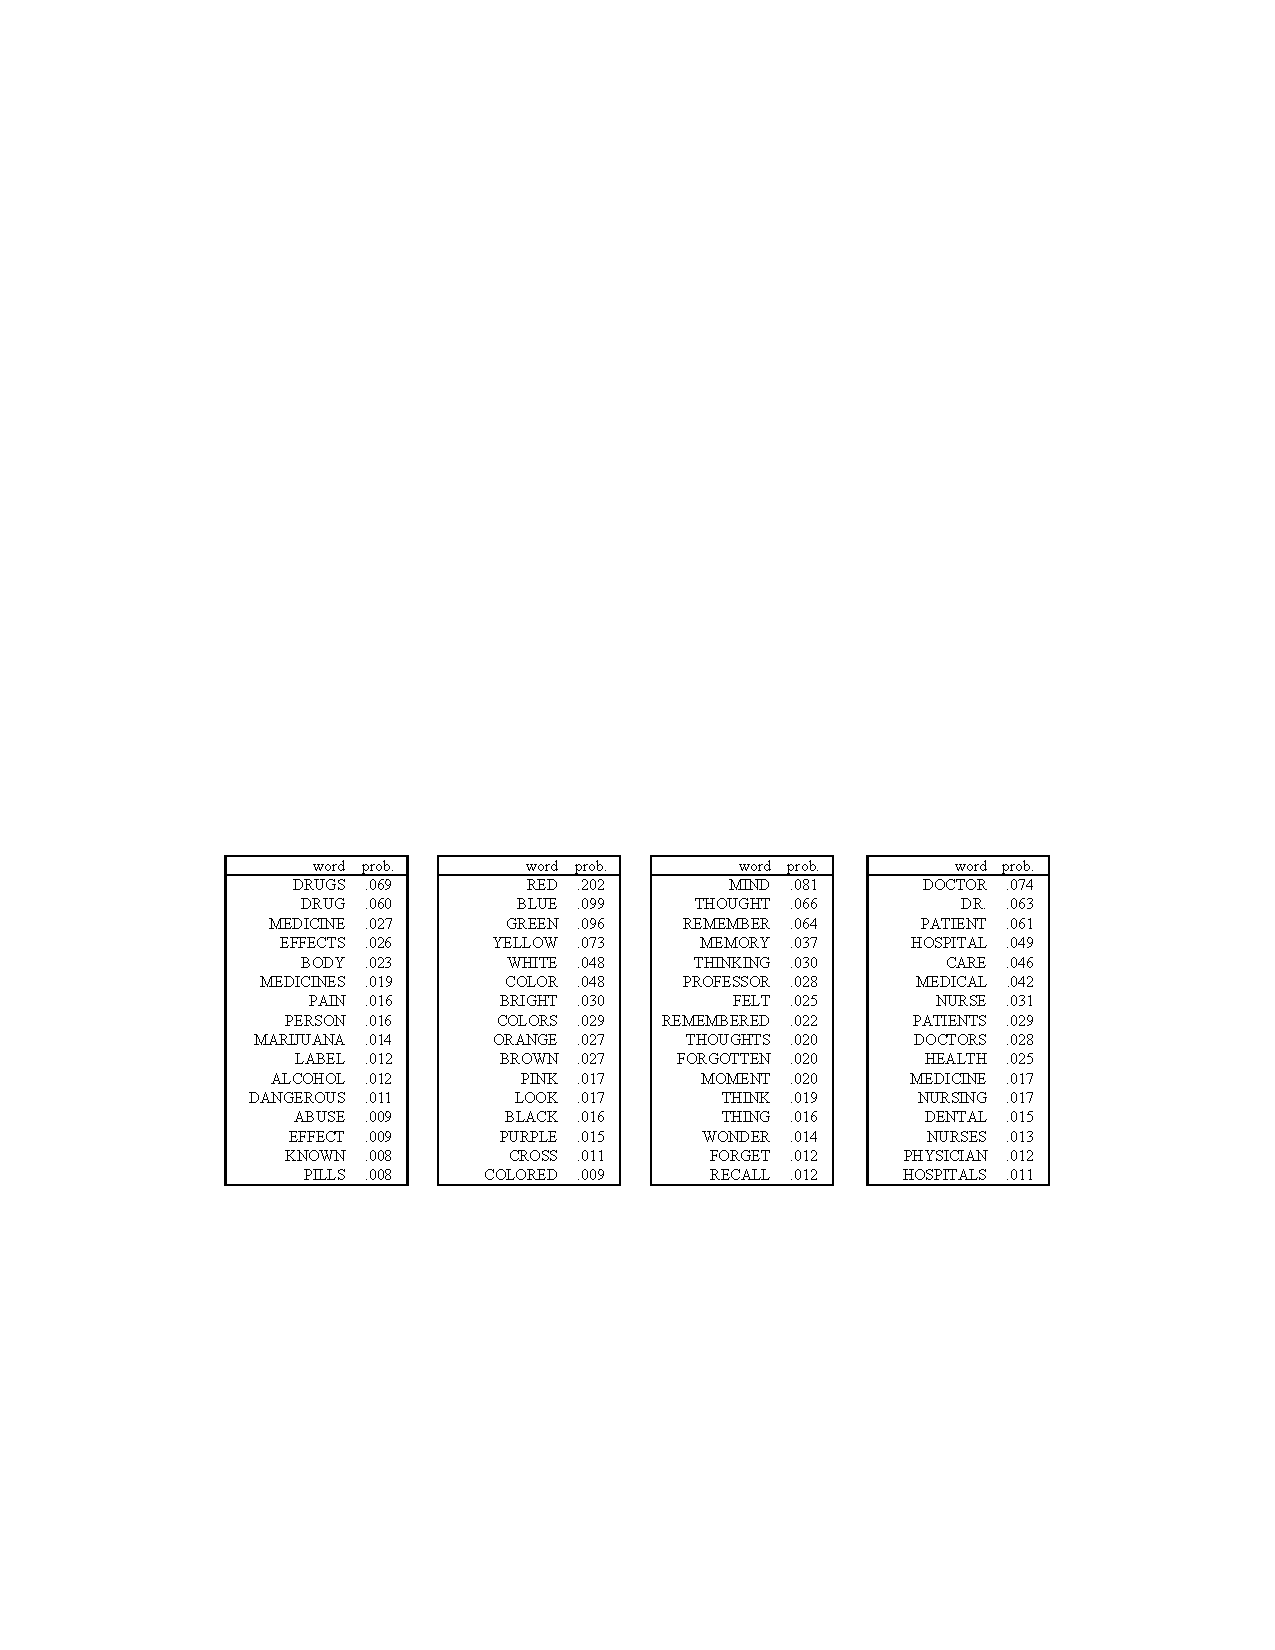
\includegraphics[scale=1]{Images/SteyversGriffithsTopics.pdf}
	\label{fourtopics}
\end{figure}

The generative model underlying topic models is based on probabilistic sampling rules and specifies how the words in documents are generated on the basis of latent variables. Given the definition of topics as word distributions, the model assumes that every word in a document is drawn from a topic. From which topic a word is to be drawn is determined by a distribution over topics. As such, documents with different content are generated by choosing different distributions over topics \cite[~p. 2--3]{Steyvers(2007)}. Figure \ref{genproc} illustrates the process of generating three documents from two topics. While two of the documents are generated exclusively from one topic, one document is an equal mixture of both topics. Note that words can be part of more than one topic, allowing the model to capture the multiple meanings of polysemies \cite[~p. 2--3]{Steyvers(2007)}.

The generative process can be inverted to appear as a problem of statistical inference (see Figure \ref{genproc}): When fitting the generative model, the aim is to identify the latent variables, here the latent topics, that are best able to explain the observed data. Thus the model is able to infer the probability distributions over words and the distribution over topics for each document from the text data \cite[~p. 3]{Steyvers(2007)}. While the inferred distributions over words are interpreted as topics, the probability distribution over topics can be usefully thought of as the extent to which a topic accounts for the content of a document. That is, the fraction of words in document $d_i$ generated by topic $\theta_j$. Note that the probabilities of document $d_i$ covering topic $\theta_{j}$ sum to one across all topics:
$$
\sum_{j=1}^{k} \pi_{ij} = 1.
$$
Thus, the topics $\{\theta_1, ..., \theta_k\}$, as inferred by the topic model, account for every word in the document, with no words being attributed to other topics \cite[pp.~338]{Zhai.2016}. 

\begin{figure}
	\caption{The generative model and the problem of statistical inference \cite[p.3]{Steyvers(2007)}.}
	\centering
	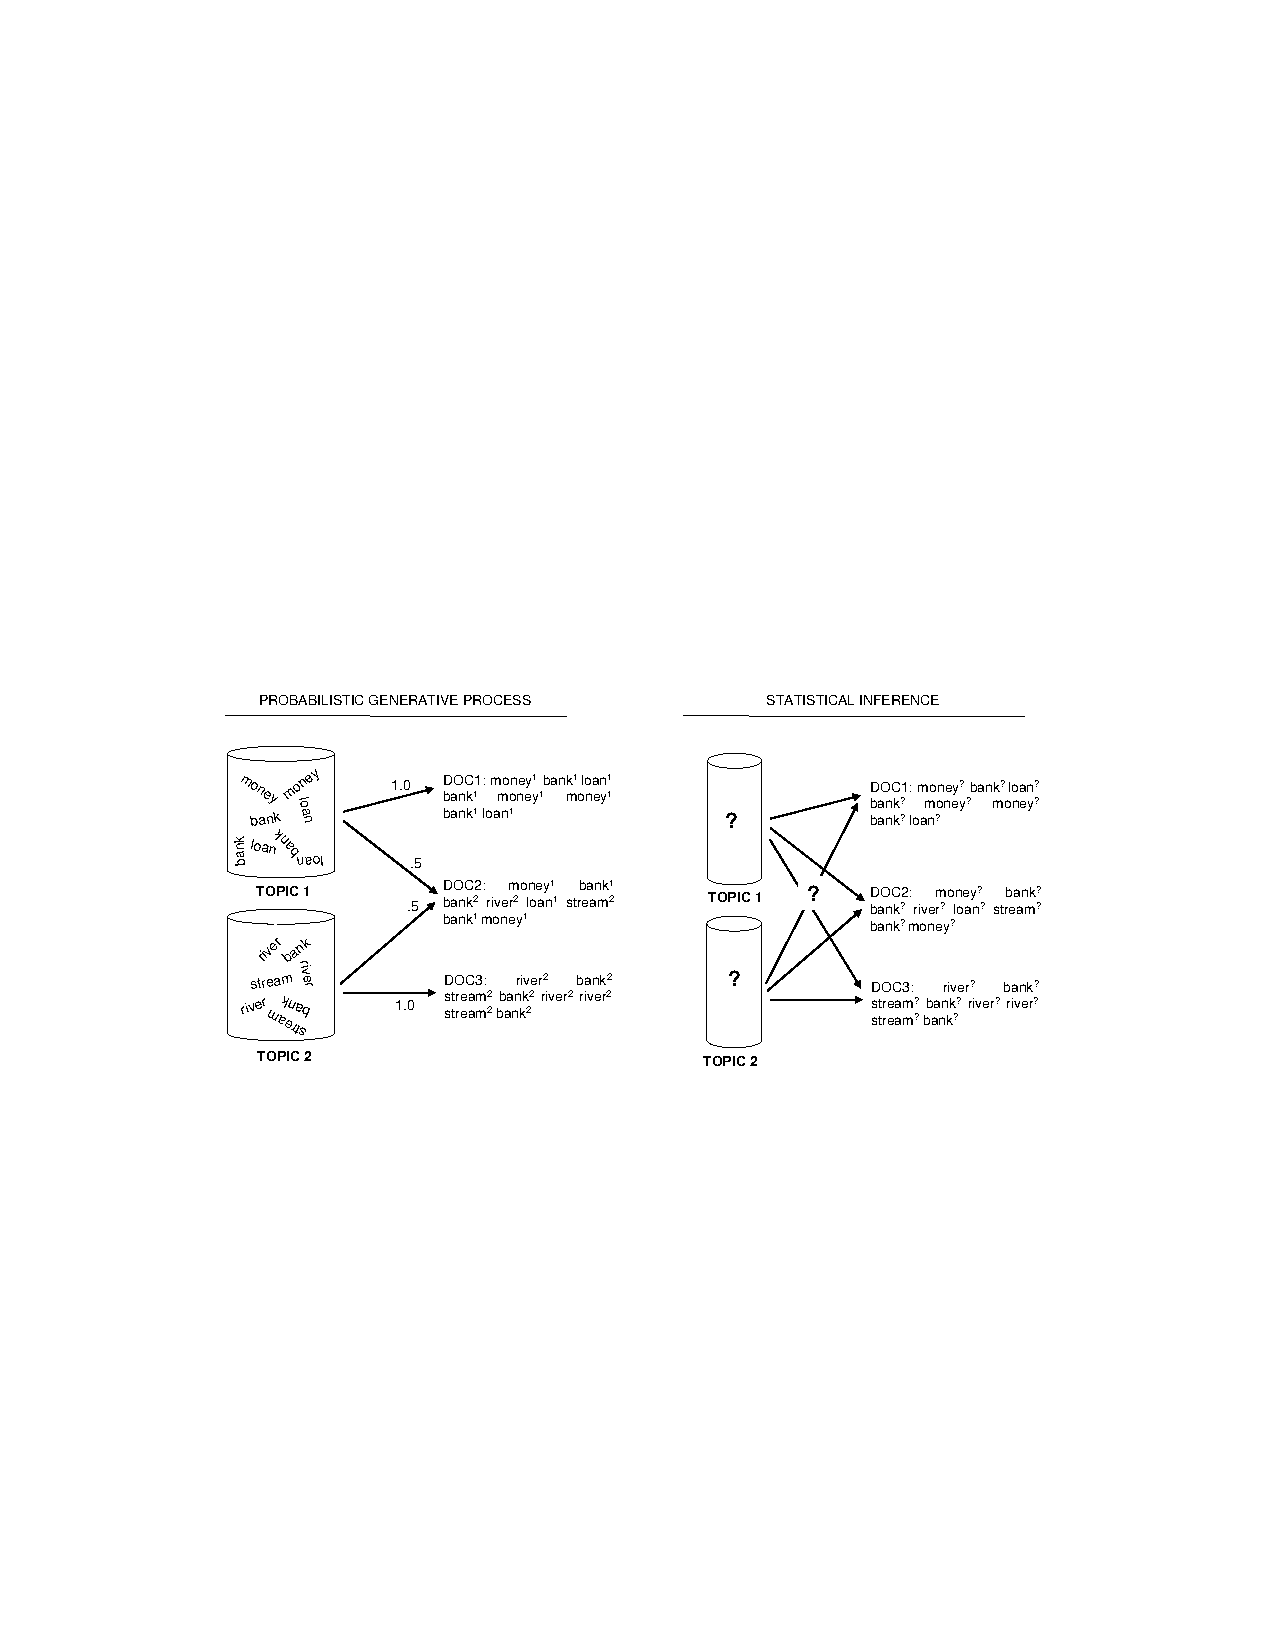
\includegraphics[scale=1]{Images/genproc.pdf}
	\label{genproc}
\end{figure}

There is one key assumption underlying the generative model: It is assumed that the order of the words in a document as well as the order of the documents in a collection can be neglected. The model picks up on the frequencies of words, but completely ignores the position of the words in the text. Should the order of the words contain useful information, it is discarded by probabilistic topic models. This assumptions is known as the “bag-of-words” assumption, an assumption of exchangeability of the the words in a document (\citealt[p.~994]{Blei.2003}; \citealt[~p. 3]{Steyvers(2007)}). \citet[~p. 290]{Hofmann.1999} himself admits that the "key assumption is that the simplified 'bag-of-words' [...] representation of documents will in many cases preserve most of the relevant information." In Figure \ref{genproc}, this principle is captured by illustrating topics as bags containing different distribution over words. The position of the words is arbitrary.
 
\section{Model Fitting with Expectation-Maximization}\label{Ch:model}

As outlined above, a topic model is a mixture model that consists of several (latent) variables, i.e. word distributions. An estimation of the model's variables is obtained via Maximum Likelihood (ML) estimation. If a mixture model consists of several components, that is more than just one topic, there is no analytical solution to the ML estimation and a numerical optimization algorithm must be employed. The Expectation-Maximization algorithm (EM) is a family of useful algorithms to obtain an ML estimate of mixture models \cite[~p. 359]{Zhai.2016} According to \citeauthor{Hofmann.1999} (\citeyear[p. 290]{Hofmann.1999}; \citeyear[p. 181]{Hofmann.2001}), EM is the "standard procedure for maximum likelihood estimation in latent variable models." 

In a first step, the ML estimation problem is to be defined. Based on the generative model outlined in Chapter \ref{GM}, the likelihood function is derived. Recall that $p(w | \theta_j)$ is the probability of word $w$ in the word distribution $\theta_j$ and that $\pi_{d,j}$ is the coverage of topic $\theta_j$ in document $d$. When faced with the problem of statistical inference, $\pi_{d,j}$ can be thought of as the probability of topic $\theta_j$ generating word $w$. Then, the probability of observing the sequence of words that make up document $d$ is:
\begin{align}
\label{prob} p(d) &= \underset{w \in V}\prod \left( \sum_{j=1}^{k}\pi_{d,j} \ p(w|\theta_j) \right)^{c(w,d)}\\
\label{log} \text{log} \ p(d) &= \underset{w \in V}\sum c(w,d) \ \text{log} \left( \sum_{j=1}^{k}\pi_{d,j} \ p(w|\theta_j) \right)
\end{align}

\noindent with $w$ being a unique word in the vocabulary set $V = \{w_1, w_2, ..., w_M\}$ and $c(w,d)$ being the count of word $w$ in document $d$. If we consider the entire collection of $N$ documents $C=\{d_1,...,d_N\}$, the log likelihood function is:
\begin{align}
\label{LL} \text{log} \ p(C|\pi_{d,j},\theta_j) &= \underset{d \in C}{\sum} \ \underset{w \in V}\sum c(w,d) \ \text{log} \left( \sum_{j=1}^{k}\pi_{d,j} \ p(w|\theta_j) \right)
\end{align}

%\noindent with $\Lambda$ denoting the unknown parameters $\pi_{d,j}$ and $\theta_j$, $j\in[1,...,k]$.

A few words of explanation. $\sum_{j=1}^{k}\pi_{d,j} \ p(w|\theta_j)$ denotes the probability of word $w$ occurring once in document $d$. It is the probability of observing the word regardless of which topic is used. We assume independence in generating each word, hence the probability of the document equals the product of the probability of each word in the document (see Eq. \ref{prob}). Eq. \ref{log} is the log likelihood function for document $d$, just as Eq. \ref{LL} is the log likelihood for the entire collection $C$ (\citealp{Hofmann.1999}; \citeyear{Hofmann.2001}; \citealp{Steyvers(2007)}; for notation see \citealp[~p. 340--377]{Zhai.2016}).

With the likelihood function defined, we are faced with a constrained optimization problem:
\begin{align}\label{argmax}
 & \underset{\pi_{d,j} \ \theta_j}{\text{arg max}} \ p(C|\pi_{d,j},\theta_j) &\\
\label{constraints} \text{s. t. } & \underset{w \in V}{\sum} \ p(w | \theta_j) = 1, \  j \in [1,k] &  \sum_{j=1}^{k} \pi_{dj} = 1, \ d \in C
\end{align}

All that is left to do is to solve the maximization problem. If we knew from which topic a word is generated it would be straightforward to calculate the ML estimate. In such a case, the word distributions would simply be the normalized word frequencies (see Chapter \ref{Ch:background} for elaborations on unigram language models). However, the partitioning of the words among the topics is not known, that is we do not know from which topic a word is generated. Therefore, we have to fall back on an iterative algorithm to solve the maximization problem. The EM algorithm proceeds by guessing from which distribution a word is generated using a tentative estimate of the parameters. Based on the assumed partitioning, the estimate of the parameters is updated. This, in turn, allows an improved inference of the partitioning, leading to an iterative hill-climbing algorithm that improves the estimate of the parameters until it reaches a local optimum \cite[p. 360]{Zhai.2016}. The algorithm proceeds in two steps: In the expectation step (E), posteriori probabilities for the latent variables are computed based on current estimates. In the maximization step (M), the parameters are updated (\citealp[p. 290]{Hofmann.1999}; \citeyear[pp. 181--182]{Hofmann.1999}). 


In the E-step, the algorithm uses Bayes rule to infer the topic that has been used to generate a word. We introduce a hidden variable $z_{d,w} \in \{1,2,...,k\}$ to capture this information. The value of this hidden variable is inferred based on a tentative set of parameters (\citealp[p. 290]{Hofmann.1999}; \citeyear[p. 182]{Hofmann.2001}; \citealp[pp. 362--374]{Zhai.2016}):
\begin{align}\label{E1}
p(z_{d,w}=j)=\frac{\pi_{d,j}^{(n)}p^{(n)}(w|\theta_j)}{\sum_{j=1}^{k}\pi_{d,j}^{(n)}p^{(n)}(w|\theta_j)}
\end{align}

Eq. \ref{E1} shows the E-Step of the EM algorithm for PLSA, where $p(z_{d,w}=j)$ is the probability that word $w$ in document $d$ is generated from topic $\theta_j$. Note that this probability depends on the document $d$, i.e. whether a word has been generated from a specific topic depends on the document. As a result, each document will have a different topic distribution, $\pi_{d,j}$, indicating the varying emphasis on specific topics across documents. I will use this fact to classify articles according to different narratives (see Chapter \ref{appPLSA}). The probability value of $z_{d,w}$ is calculated for every unique word in each document by computing the product of the probability of word $w$ given the selected topic and the probability of selecting a topic. The product is normalized to ensure the constraints in Eq. \ref{constraints} hold. The superscript $^{(n)}$ indicates the generation of parameters in the iteration \citep[pp. 374--376]{Zhai.2016}.  

In the M-step we calculate an ML estimate of the parameters $\pi_{d,j}$ and $p(w|\theta_j)$ using the estimate obtained in step E. We use the estimated partitioning of the words among the topics to adjust the word count $c(w,d)$, that is we obtain a discounted word count $c(w,d) p(z_{d,w}=j)$ which can be understood as the expected count for the event that word $w$ is generated from $\theta_j$. Remember that the ML estimation could not be solved analytically because we did not know the partitioning of the words. Having obtained a tentative guess of the partitioning, we can easily estimate $\pi_{d,j}$ (the probability of document $d$ covering topic $\theta_j$) and $p(w|\theta_j)$ (the probability of word $w$ for topic $\theta_j$) (\citealp[p. 290]{Hofmann.1999}; \citeyear[p. 182]{Hofmann.2001}; \citealp[pp. 364--375]{Zhai.2016}):
\begin{align}%\label{M1}
\label{M1pi} \pi_{d,j}^{(n+1)}=\frac{\sum_{w \in V} c(w,d)\ p(z_{d,w}=j)}{\sum_{j \in k}\sum_{w \in V}c(w,d) \ p(z_{d,w}=j)}\\
\label{M1theta} p^{(n+1)}(w|\theta_j)=\frac{\sum_{d \in C} c(w,d)\ p(z_{d,w}=j)}{\sum_{w \in V}\sum_{d \in C}c(w,d)\ p(z_{d,w}=j)}
\end{align}

As Eq. \ref{M1pi} and Eq. \ref{M1theta} illustrate, the computation of the parameter estimates amounts to no more than aggregating the the expected word counts and normalizing them among all topics or among all words, respectively. The normalization must ensure that the constraints in Eq. \ref{constraints} hold. The new generation of parameters is used to adjust the probabilities of the $z_{d,w}$ values, which subsequently can be used to compute a next generation of parameters. The EM algorithm continues to iterate over the E- and M-step until the likelihood converges. Instead of using a convergence condition, a stopping rule can be employed. In this case, the algorithm stops updating the parameters once a sufficient performance, as defined in the stopping criterion, is reached \citep[pp. 182--183]{Hofmann.2001}. 

As mentioned before, EM is a hill-climbing algorithm that starts with an initial guess of the parameter values and then successively improves it. In the process of improving the estimate, the EM algorithm is guaranteed to converge to a local, but not a global maximum. To account for this, \citeauthor{Zhai.2016} recommend applying the algorithm repeatedly with changing initial values for the unknown parameters and using the run with the highest likelihood value (\citeyear[pp. 363--368]{Zhai.2016}).\footnote{For more details on the properties of EM, see Chapter 9 in \cite{Bishop.2006}.}

\section{Adding a Background Language Model}\label{Ch:background}


In the original PLSA (\citealp{Hofmann.1999}; \citeyear{Hofmann.2001}) as it was introduced in Chapter \ref{Ch:model} there is no background topic. The model contains $k$ topics, $\{\theta_1, ..., \theta_k\}$, that are treated as unknown and inferred via a probabilistic process. As a result, very common words will show up prominently in the learned topics. Yet, common words often carry very little relevant information, such as stop words (more on stop words in Chapter \ref{preprocessing}). 
The aim of a background topic is to represent the common words in the text data so that the learned topics can capture the content-bearing words and the statistical semantic word patterns of interest are revealed \cite[pp.7--8]{Darling.2011}. 

An example of a probabilistic topic model that includes background distributions is \citeauthor{Chem.2007}'s (\citeyear{Chem.2007}) special words with background model (SWB). It is an extension to LDA which allows words in a document to be modeled as either originating from general topics, or from document-specific “special” word distributions, or from a corpus-wide background distribution. However, a simpler approach, where only one background distribution is added to LDA, is possible as well, as \citet[pp.7--8]{Darling.2011} demonstrates. Analogously to \cite{Darling.2011}, I add a single background distribution to my PLSA model.

Let's look at the behavior of a mixture model to understand the usefulness of a background model. Topics are word distributions with the simplest word distribution being the unigram language model. We assume that words in a text are generated independently. Thus, the likelihood of a sequence of words is equal to the product of the probability of each word \citep[pp. 51--54]{Zhai.2016}. Assume that $\theta$ is the single topic to be inferred from document $d$. Then the ML estimation problem is given by
\begin{align}
\label{ul} & p(d|\theta) = \underset{w \in V}\prod p(w|\theta)^{c(w,d)}\\
\label{constraintsul} & \text{s. t. } \underset{w \in V}{\sum} \ p(w|\theta) = 1
\end{align}
the solution to which is
\begin{align}
\label{estul} & \ p(w_i|\hat{\theta}) = \frac{c(w_i,d)}{|d|}
\end{align}
where $c(w,d)$ is the word count in document $d$ and $|d|$ is the total number of words in document $d$ \citep[pp. 341-343]{Zhai.2016}. 

Eq. \ref{estul} illustrates that the ML estimator of a unigram language model gives each word a probability equal to its relative frequency in the document. Consequently, only observed words have a non-zero probability while words that do not show up have zero probability. Further, a very high probability is given to words that show up frequently. The more prominent a word, the higher its probability in the word distribution. 
%This allows a unigram language model to perform semantic analysis as it picks up on words that show up frequently in the same document. Such words will have a similar probability due to their co-occurrence and thus a semantic association is assumed, leading to the mining of a topic. 
However, usually functional words and stop words are used the most frequently in a text and thus will have high probabilities, while content-carrying words will have a much lower probability. Thus, a topic can be completely dominated by uninformative words. Introducing a background language model can help filter out such words \citep[pp. 51--54]{Zhai.2016}.  

To change the predominance of common words, the generative process needs to be adjusted so that the learned topics do not have to generate these words. Specifically, another word distribution that generates the common words, called the background topic ($\theta_B$), has to be introduced. A natural choice for the background topic is the unigram language model because it assigns high probabilities to frequent words. Including a background model in the mixture model will allow the learned topics to assign high probabilities to content-carrying words instead (\citealp[pp.7--8]{Darling.2011}; \citealp{Chem.2007}).  

Consider the optimization problem of a mixture model in Eq. \ref{argmax} and Eq. \ref{constraints}. In order to maximize the overall likelihood, different topics tend to put a high probability on different words. Put differently, when a word, $w_1$, is assigned a high probability in one word distribution, $w_1$ will tend to have a low probability in another distribution. That is, if $p(w_1|\theta_j)$ is high, then $p(w_1|\theta_i)$ tends to be low, and vice versa. Thus, the behavior of a mixture model ensures that when a background model is introduced that puts high probabilities on common words, the other distributions are encouraged to put a low probability on common words and more probability mass on words that rank low in the background distribution. Of course, due to the nature of the ML estimate of a mixture model, if a word appears very frequently in the text, it will tend to have a high probability in all distributions as this optimizes the overall likelihood \citep[pp. 353--359]{Zhai.2016}.

If a background topic is introduced into the mixture model, a decision needs to be made as to whether a word is generated by the background model, $\theta_B$, or by one of the learned models, $\theta_i$. This choice is controlled by a probability distribution over the components of the mixture models: $\lambda_B$ denotes the probability that the background model was used to generate a word. The likelihood function is given by \citep[p. 372]{Zhai.2016}:
\begin{align}
\label{BLL} \text{log} \ p(C|\pi_{d,j},\theta_j) &= \underset{d \in C}{\sum} \ \underset{w \in V}\sum c(w,d) \ \text{log} \left( \textcolor{blue}{\lambda_B p(w|\theta_B) + (1-\lambda_B)} \sum_{j=1}^{k}\pi_{d,j} \ p(w|\theta_j) \right)
\end{align}

The difference to the likelihood function in Chapter \ref{Ch:model} is marked in blue. The ML estimation problem remains unchanged (see Eq. \ref{argmax} and Eq. \ref{constraints}). Note that the probability of observing a word from the background distribution is $\lambda_B \ p(w|\theta_B)$ while the probability of observing a word from the learned topic $\theta_j$ is $(1-\lambda_B) \ p(w|\theta_j)$. The background model, $\theta_B$, is assumed to be known and can, for instance, be estimated as a unigram language model of the collection. This is powerful way to introduce domain knowledge about the text into the model \citep[pp. 352, 372--376]{Zhai.2016}. 

Consider how the probability of choosing the background model $\lambda_B$ influences the maximization problem. The higher the probability of choosing the background model is, the higher is the probability mass on the words in the background model $\lambda_B  p(w|\theta_B)$.  The opposite is true for learned topics as $(1-\lambda_B)  p(w|\theta_j)$ will be lower the higher $\lambda_B$. As a result, inferred distributions will give a low probability to common words because they have a high probability in the background topic. Instead, the learned topics will give other, content-bearing words a higher probability. The higher $\lambda_B$, the more common words are filtered out from the learned topics $\{\theta_1, ..., \theta_k\}$ \citep[pp. 352--359]{Zhai.2016}.  

$\lambda_B$ indicates the fraction of words generated from the background model. This parameter needs to be specified and can be understood as a prior in the process of Bayesian inference. It encodes a prior belief about the partitioning of the words between the background and the learned topics and thus again allows us to introduce domain knowledge that we may have about the text \citep[pp. 361, 372--376]{Zhai.2016}. 

Based on Eq. \ref{BLL} the EM algorithm looks as follows:
\begin{align}\label{BE1}
p(z_{d,w}=j)&=\frac{\pi_{d,j}^{(n)}p^{(n)}(w|\theta_j)}{\sum_{j=1}^{k}\pi_{d,j}^{(n)}p^{(n)}(w|\theta_j)}\\
\label{BbE1}
\textcolor{blue}{ p(z_{d,w}=B)} & \textcolor{blue}{ =\frac{\lambda_B \ p(w|\theta_B)}{\lambda_B \ p(w|\theta_B) + (1-\lambda_B) \sum_{j=1}^{k}\pi_{d,j}^{(n)}p^{(n)}(w|\theta_j)} }
\end{align}
Eq. \ref{BE1} and Eq. \ref{BbE1} show the E-Step of the EM algorithm for PLSA with a background model, where $p(z_{d,w}=j)$ is the probability that word $w$ in document $d$ is generated by topic $\theta_j$ (conditional on not being generated by the background model) and $p(z_{d,w}=B)$ is the probability of $w$ being generated by the background model $\theta_B$. The M-step is:

\begin{align}%\label{M1}
\label{BM1pi} \pi_{d,j}^{(n+1)}=&\frac{\sum_{w \in V} c(w,d) \ \textcolor{blue}{(1-p(z_{d,w}=B))}\ p(z_{d,w}=j)}{\sum_{j \in k}\sum_{w \in V}c(w,d) \ \textcolor{blue}{(1-p(z_{d,w}=B))} \ p(z_{d,w}=j)}\\
\label{BM1theta} p^{(n+1)}(w|\theta_j)=&\frac{\sum_{d \in C} c(w,d) \ \textcolor{blue}{(1-p(z_{d,w}=B))} \ p(z_{d,w}=j)}{\sum_{w \in V}\sum_{d \in C}c(w,d)\ \textcolor{blue}{(1-p(z_{d,w}=B))}\ p(z_{d,w}=j)}
\end{align}
As before, in the M-step we use a tentative partitioning of the words, as derived in the E-step, to update the parameters. Now, however, words are partitioned among the $k$ inferred topics, $\{\theta_1, ..., \theta_k\}$, conditional on not being allocated to the background topic \citep[pp. 372--376]{Zhai.2016}. 

Note that the PLSA model with a background topic is the more general case. By setting $\lambda_B=0$ we arrive at the formulae for the PLSA model without background distribution. If $\lambda_B=1$, the background topic is an infinitely strong prior that leaves no room for other topics. This is in line with the intuitive understanding of $\lambda_B$ as the fraction of words that are generated by the background topic. 



\chapter{Data and Methodology}

This chapter gives an overview of the data used in this thesis. The financial data set is outlined in Chapter \ref{Ch:financedata}, the text data set in Chapter \ref{textdata}. Further, Chapter \ref{methodology} explains how the data was processed and applied to the topic modeling task.  

\section{Financial Data}\label{Ch:financedata}

Data on target rate adjustments and FOMC meetings was retrieved from the Fed's website (\citealp{FRS.2018}, \citeyear{FRS.2013}; \citealp{FOMC.2018Archive}; \citeyear{FOMC.2018}) and summarized in table \ref{tab:meetings} and \ref{tab:target} in Appendix \ref{AppendixA}. 

The FOMC holds eight regularly scheduled meetings during the year. Additional, unscheduled meetings are called when necessary \citep{FOMC.2018}. In April 2011, the Fed has taken up the practice of holding quarterly press conferences where it comments on its policy decisions, including its treatment of the target rate. Usually, the press conferences take place after every other meeting. In June 2018, the Fed announced that starting January 2019 it will hold a press conference after every meeting \citep{PressConference.2018}. Table \ref{tab:meetings} in Appendix \ref{AppendixA} lists all 195 FOMC meetings that have taken place over the last 20 years. If a meeting lasted two days, only the last day is listed. Unsurprisingly, certain years necessitated more emergency meetings than others: In 2008, the FOMC held a total of 14 meetings, 6 more than usual. In 2001, the FOMC held 13 meetings, two of which were conference calls shortly after the events of 9/11. While the market anticipates the scheduled meetings and forms expectations about potential policy actions, the same is not possible for unscheduled emergency meetings. 

Table \ref{tab:target} in Appendix \ref{AppendixA} gives an overview of the changes in the target rate over the past 20 years. From January 1998 to September 2018, the target rate was adjusted on 57 occasions. Only six of the 57 adjustments happened after unscheduled meetings. Most notably, two surprise adjustments took place during 2008 and three during 2001, one of them shortly after 9/11. Until 2008, the Fed used to decide and implement the new target rate on the very same day. The practice was changed after 2008 and the target rate was subsequently adjusted on the day following the FOMC meeting. 

The development of the target rate over time is characterized by periods of stark increase and decrease. In May 2000, the target rate was at its highest with 6.5\%. From January 2001 to June 2003, the target rate decreased steadily until it reached a low point of 1\%. Mid-2006, the target rate was again at 5.25\% but was lowered drastically in 2007 and 2008 until it reached its all-time low of 0\% in December 2008. At the same time, the FOMC introduced a target range and defined the target rate no longer as a discrete number but with the help of an upper and lower bound. For seven years, until december 2015, the FOMC kept the target rate in the range of 0\% to 0.25\%. Since then, it has slowly increased the target rate, announcing a range of 2\%--2.25\% in September 2018.
%
%\begin{figure}
%	\caption{Target rate and 3M treasury yield.}
%	\centering
%	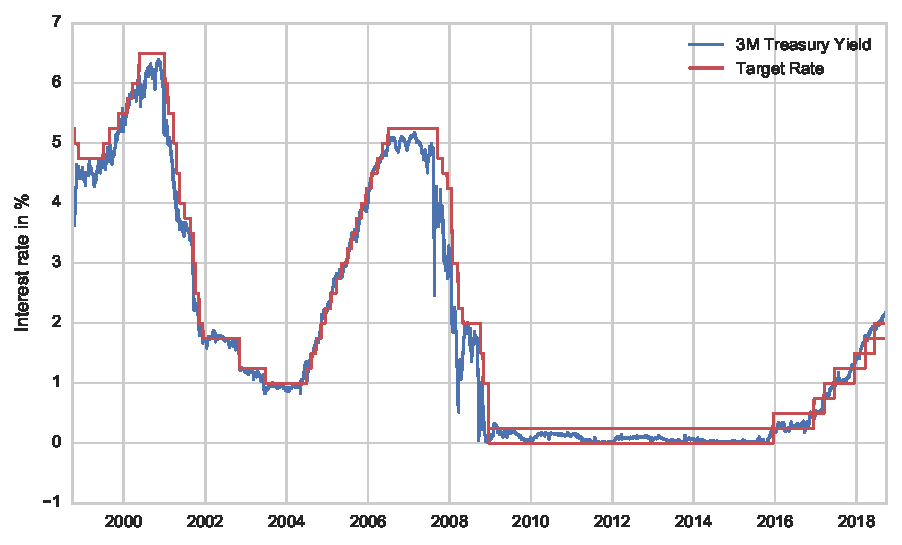
\includegraphics[scale=1]{Images/3Mtreasury.pdf}
%	\label{3Mtreasury}
%\end{figure}

The daily yield curve of the US Treasury bills, notes, and bonds for the period of October 1, 1998 to September 30, 2018 was retrieved from Thomson Reuters Datastream. Figure \ref{3Mtreasury} illustrates the development of the 3-month treasury yield as well as the target rate over the 20-year period. As explained in Chapter \ref{ExistingResearch}, \citeauthor{Ellingsen.2003} approximate unexpected monetary policy actions with the change in the 3-month T-bill rate. They argue, that the 3-month rate is sufficiently short to be determined by the target rate, but also sufficiently long to avoid noise from expectation errors \citep[~p. 13]{Ellingsen.2003}. Indeed, Figure \ref{3Mtreasury} shows that the 3-month T-bill rate and the target rate seem to move in tandem.  

The treasury yields for all other maturities are depicted in Figure \ref{alltreasury} in Appendix \ref{AppendixA}. Please note that for the 1-month rate the data series starts on July 31, 2001 and for the 7-year rate the series starts on May 26, 2009. Due to data availability, the 20-year rate is given as a constant maturity rate while the rates of the other maturities are given as bid yields. As expected, while the short term yields (up to 1 year) move quite closely with the target rate, the longer the maturity the more it emancipates itself from the target rate. 

%The bid yield is the yield figure that you get when you consider what your long-term return would be if you paid the bid price for the bond. 
%Bid yields are always higher than ask yields, because if the buyer were willing to take a yield that was equal to or less than the ask yield, then the seller would sell the bond to the buyer at that corresponding price. 
%Constant maturity is the theoretical value of a U.S. Treasury that is based on recent values of auctioned U.S. Treasuries. The value is obtained by the U.S. Treasury on a daily basis through interpolation of the Treasury yield curve which, in turn, is based on closing bid-yields of actively-traded Treasury securities. It is calculated using the daily yield curve of U.S. Treasury securities.

\begin{figure}
	\caption{Target rate and 3M treasury yield.}
	\centering
	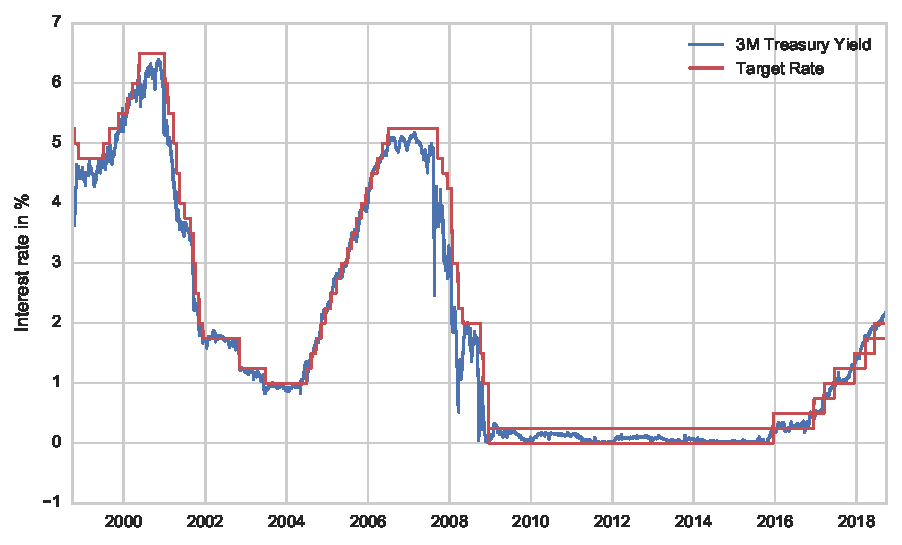
\includegraphics[scale=1]{Images/3Mtreasury.pdf}
	\label{3Mtreasury}
\end{figure}

\section{Text Data}\label{textdata}

Articles are collected from the Dow Jones Factiva Database\footnote{https://global.factiva.com} by use of the search terms \textit{Federal Reserve} and \textit{interest rate}. Only articles that appeared in the \textit{United States} on the subject of \textit{interest rates} in a window of three days around each target rate adjustment (the day before, of, and after an adjustment as listed in Table \ref{tab:target}) are taken into account. The articles are mainly taken from the \textit{The Wall Street Journal}, \textit{Financial Times}, \textit{Reuters}, \textit{The Associated Press}, \textit{Market News International}, \textit{Dow Jones Institutional News}, \textit{Agence France}, and \textit{AFX}, as these newspapers seem to publish the most articles on the topic. 

From October 1, 1998 to September 30, 2018, 56 target rate adjustments have taken place, for which a total of 2'318 articles have been extracted. Since the FED changed its policy from undertaking a target rate change on the same day as a FOMC meeting to only doing so on the following day, articles $\pm1$ day around the official target rate change have been collected. This ensures that the articles capture any information, speculation, and interpretations that abound directly after the meeting, on the day of the target rate change as well as on the following day. On rare occasions, the number of articles ran in the several hundreds and only the most relevant have been selected. 

The final sample comprises between 14 and 97 publications for every policy day. In total, over $1'600'000$ tokens are extracted from these articles. After stop words have been removed, the token count drops to roughly $850'000$. For more information on text preprocessing, see Chapter \ref{preprocessing}. Figure \ref{tokencount} in Appendix \ref{AppendixB} illustrates the spread of the text data across policy days and shows that the token count fluctuates quite drastically. More data is available for recent target rate adjustments, less for more historic adjustments.

Looking at the most common words in the entire text data base, as illustrated in Figure \ref{wcloud}, yields no surprises. As one might expect, the articles make heavy use of context specific vocabulary such as "interest rate", "federal reserve", "economy", but also of terms appropriate for a financial environment such as "basis point", "percentage point", or "investor". Even analyzing just the headlines of the articles yields an almost identical word usage. %Thus, headlines appear to be just as factual and technical as the general text body. Overall, this is a first indication that while there is a set vocabulary to talk about the facts of a target rate change, there is no similarly systematic vocabulary to express interpretations and sentiments surrounding such a change. 

\begin{figure}
	\caption{Wordcloud illustrating the most common words across all articles.}
	\centering
	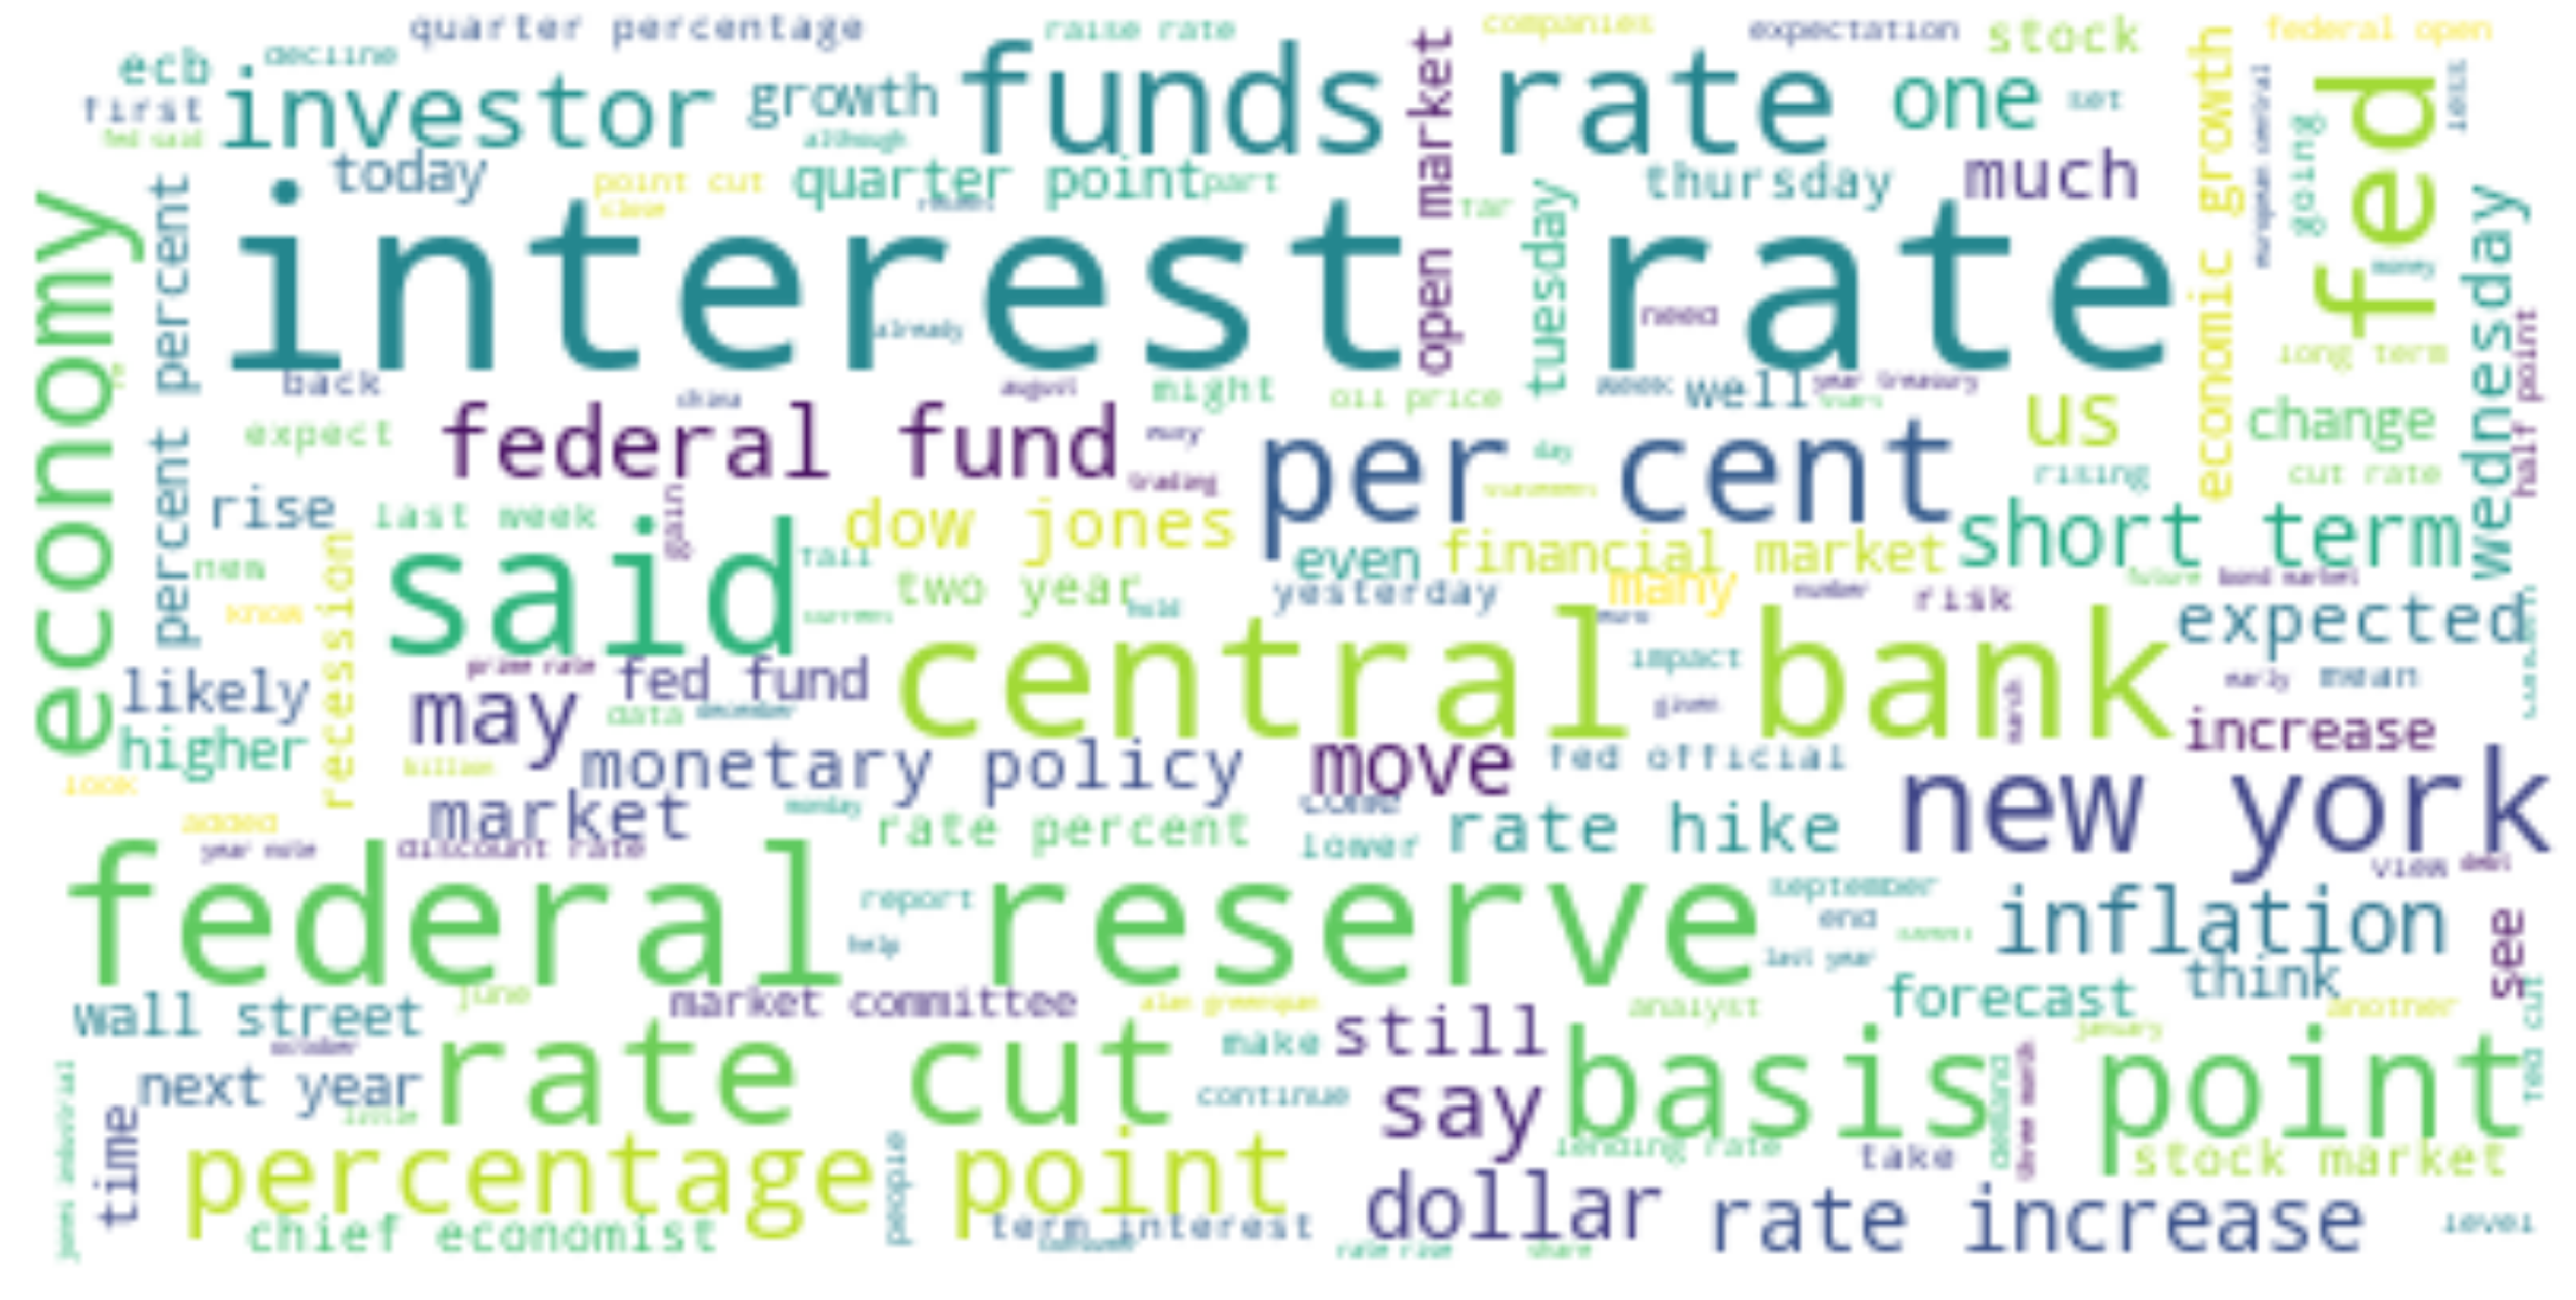
\includegraphics[scale=0.2]{Images/wordcloud.pdf}
	\label{wcloud}
\end{figure}

A closer look at the dispersion of the most common words reveals that their usage is consistent over time (see Figure \ref{dispersion}\footnote{A remark on the label of the x-axis: The x-axis tracks the token count of the entire text data and the diversion plot indicates at which token count the word of interest has been found. However, displaying the token count at which a word is found has little meaning. Thus, the x-axis displays the progression of years in which the articles were published. Since the tokens are not spread smoothly across the years, the intervals are irregular.}). The frequently used terms are just as likely to be used in older articles as in newer publications. As one might expect, the articles talk about "rate cut" in times where the Fed is lowering the target rate, and about "rate increase" when the Fed is in the process of raising the target rate.

\begin{figure}
	\caption{Dispersion of most common words across time.}
	\centering
	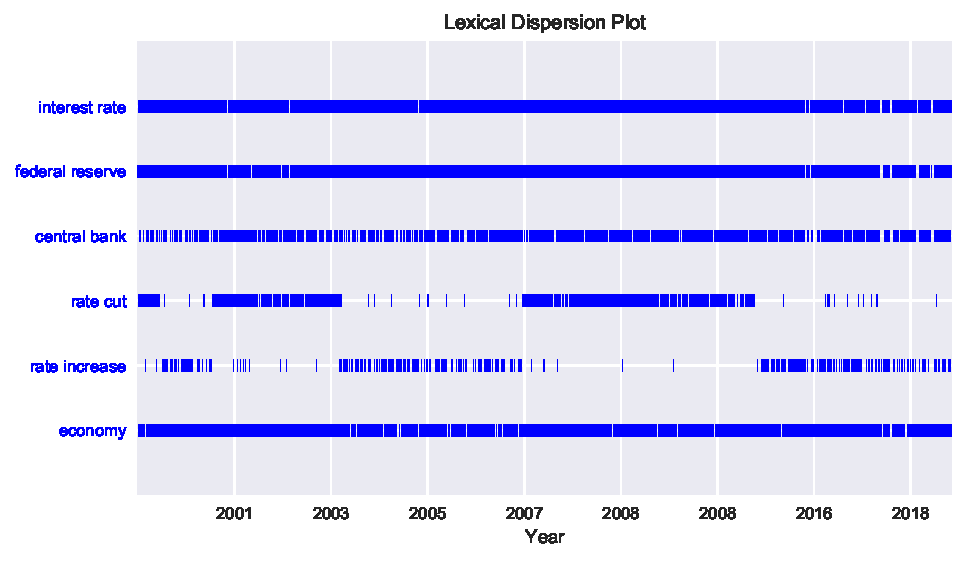
\includegraphics[scale=1]{Images/dispersionplot.pdf}
	\label{dispersion}
\end{figure}

	
%More than 100 articles, needed selection: 15.12.2016 / 17.12.2015 / 22.01.2008 / 18.09.2007/ // 08.10.2008 corrupted file! - no wall street journal//


\section{Methodology}\label{methodology}

This Chapter explains the preprocessing of the text data (Chapter  \ref{preprocessing}), the engenieering of the feature space (Chapter \ref{featueeng}) and the application of the PLSA model with and without background topic (Chapter \ref{appPLSA} and \ref{Ch:implembg}).


\subsection{Text Preprocessing}\label{preprocessing}
Text data in its raw form contains all the ambiguities that are inherent in natural language. Thus, before any NLP tasks can be performed, the text data needs to be prepared. Text preprocessing is the process of converting raw text into "a well-defined sequence of linguistically meaningful units." This part of the NLP process is essential, as any analysis that follows is based on the linguistic units (characters, words, and sentences) identified at this stage \cite[p. 9]{Palmer.2010}. Topic models in particular are sensitive to preprocessing as they rely on a sparse vocabulary \cite[p. 288]{Schofield.2016}.

Recall that topic models rely on the "bag-of-words" assumption and neglect the order of words in a text as well as the order of documents in a corpus. Therefore, the main task of the preprocessing stage is the correct identification of words as the linguistically meaningful units to be used in topic modeling. \citet[p. 10]{Palmer.2010} refers to the process of converting text data into its components as text segmentation. In particular, the process of breaking up a sequence of characters at the word boundaries is called word segmentation. Words identified by word segmentations are known as tokens and the process of identifying them is also known as tokenization \citep[p. 10]{Palmer.2010}.

\citet[pp. 16-19]{Palmer.2010} rightly points out that there exists plenty of tokenization ambiguity. In a language where words are generally space-delimited, a natural approach to tokenization is identifying any sequence of characters preceded and followed by a space as a token. However, this leaves a certain amount of ambiguity when it comes to punctuation and multi-word expressions. Apostrophes, for instance, are used to mark contractions, the genitive form of nouns, and even the plural form of nouns. Tokenization needs to implement a rule regarding the treatment of such ambiguous cases. Consider the example word \textit{Peter's}. In this case, \textit{'s} could indicate a possession as well as a contraction of the verb \textit{is} and it could be tokenized as \textit{Peters} or as two tokens, \textit{Peter} and \textit{'s}, or even as \textit{Peter} and \textit{is}, if that was the supposed meaning \cite[pp. 16-19]{Palmer.2010}.

\cite{Bird.2010} supply a series of word tokenizers. However, even they admit that when it comes to tokenization "no single solution works well across-the-board, and we must decide what counts as a token depending on the application domain." The problem of tokenization gets compounded by the problem of stop words. As outlined in Chapter \ref{Ch:background}, functional words occur frequently in texts and thus can clutter up the information we are trying to discover. Such stop words carry little information and obscure the analysis by crowding-out more meaningful words. It can therefore be useful to remove stop words from the text data altogether. 

To remove stop words, one can make use of publicly available lists of stop words. However, \citet{Nothman.2018} point out the difficulties and incompatibilities of such lists. Investigated the variation and consistency of several lists, they come to the conclusion that stop words are often included based on frequency statistics but also based on manual selection and filtering. Thus, lists vary greatly in the words they include. Apart from uncertainty regarding the selection of the stop words, stop lists may also assume a particular tokenization strategy. Yet, as \citet{Nothman.2018} point out, the stop lists provided by some open source libraries do not always go with the tokenizer provided by the same libraries. For example, while a tokenizer might split the word \textit{hasn't} into the tokens \textit{has} and \textit{n't}, the accompanying stop word list only contains \textit{has} and \textit{not}, omitting the token \textit{n't}. Further, several lists include the words \textit{has} and \textit{have}, but fail to list \textit{had}, letting the omission and inclusion of stop words appear arbitrary \citep[pp. 7--11]{Nothman.2018}.  

By general assumption, topic models benefit from stop word removal \cite[p. 432]{SchofieldA.MagnussonM.&MimnoD..2017}. \cite{Blei.2003}, \cite{Chem.2007}, \cite{Steyvers(2007)}, and \cite{Hofmann.2001} removed stop words during text preprocessing as so keep these words from impacting their analysis. According to popular belief, topic models benefit from manually constructed stop word lists \cite[p. 432]{SchofieldA.MagnussonM.&MimnoD..2017}. \citet[p. 7]{Darling.2011}, for instance, claims that stop lists must often be domain-specific. Contrarily, \cite{SchofieldA.MagnussonM.&MimnoD..2017} show that a domain specific approach to stop word removal is not necessary. While the removal of very frequent terms improves the quality of topic models, the removal of text specific stop words yields little benefit. If the removal of common stop words proves insufficient, unwanted terms can be removed after model training, yielding better results than ex-ante removal (\citealp[p. 432]{SchofieldA.MagnussonM.&MimnoD..2017}; \citealp{Schofield.2017}).

Another common step in the stage of preprocessing is stemming. Stemming removes the suffixes of words in order to reduce related words to an identical stem. The words \textit{happily}, \textit{happier}, and \textit{happy}, for instance, might be reduced to the same token \cite[p. 287]{Schofield.2016}. Potential advantages of stemming are an improved model fit due to a reduced feature space, improved stability in the topics due to elimination of small morphological differences, and improved interpretability due to word equivalence.  However, stemming may also render words unrecognizable (e.g. \textit{stai} as the stem of \textit{stay}), or it may lead to the incorrect conflation of unrelated words (e.g. \textit{absolutely} and \textit{absolution}), and it does not deal well with morphologically similar words that carry different meanings \cite[p. 287]{Schofield.2016}. \cite{Schofield.2016} analyze the effect of stemming in topic modeling and find that it yields little benefit and might actually be harmful. For one, stemming leads to no likelihood gains after controlling for vocabulary size. Further, the coherence of the topics is not improved by stemming. As \citet{Schofield.2017} point out, topic models are already placing morphologically similar words in the same topic, thus making stemming for the purpose of morphological conflation redundant. Lastly, strong stemming increases the model's sensitivity to random initialization as it decreases clustering consistency, that is stemming does not ensure that related words are spread across fewer topics \cite[pp. 293--295]{Schofield.2016}.  

In conclusion, \cite{Schofield.2017} recommend to pre-process lightly, that is to remove only the most frequent stop words and to omit stemming altogether, in order to avoid discarding useful text information. 

The text data used in this thesis is collected from the Down Jones Factiva Database and converted to .txt files for further processing. The metatext of all articles has been discarded so that only the main body of text and the headline remains. To segment the text into words, I apply the tokenizer provided by \cite{Bird.2010} in the nltk library. This tokenizer uses regular expressions to split the text at the word boundaries, generally treating punctuation characters as separate tokens and splitting standard contractions, i.e. \textit{don't} is tokenized as \textit{do} and \textit{n't} and \textit{children's} as \textit{children} and \textit{'s}. 

Subsequently, I filter out stop words using the stop word list for the English language provided by the nltk library \citep{Bird.2010}. The list encompasses 179 words, including common verbs, articles, prepositions, and contractions. \citet[pp. 8--9]{Nothman.2018} caution against stop lists that fail to complement the accompanying tokenizer and mention that many stop lists also tend to include controversial words, like \textit{system} and \textit{cry}. A closer examination of the nltk list reveals that the token \textit{n't} is not included in the list, even though the nltk tokenizer clearly produces it. Further, the stop word lists contains many contractions without the preceding apostrophe, even though the tokenizer joins the apostrophe and the enclitic in one token. For instance, the stop word list carries \textit{ll}, \textit{s}, \textit{d}, and \textit{ve} while the tokenizer produces \textit{'ll}, \textit{'s}, \textit{'d}, and \textit{'ve}. On the upside, the nltk list appears to carry no obviously controversial terms. I manually add the missing tokens to the stop word list before applying it. 

In line with the recommendation from \cite{Schofield.2017}, I refrain form applying a stemmer. However, I covert all characters to lower case, as to ensure that word equivalence is not hindered by capitalization. Also, I remove all non-alphabetic characters as well as tokens of length one, as numbers, punctuation marks, and single characters are of little use when it comes to topic generation and interpretation. 

After tokenization, the text data collection encompasses more than 1'600'000 tokens. After the removal of stop words, the token count drops to roughly 1'100'000 tokens. Subsequently, the non-alphabetic characters, especially the punctuations marks, are removed and the final count amounts to approximately 850'000 tokens. Thus, even though a conservative preprocessing strategy has been chosen, the text data is reduced by almost half during preprocessing (see Figure \ref{tokencount} in Appendix \ref{AppendixB}).

\subsection{Feature Engineering}\label{featueeng}
Selecting the features is the most important factor in determining the success of a statistical learning process. While machine learning models are often general, feature engineering is domain-specific and a lot of effort in any machine learning projects has to be dedicated to the construction of the feature space. At the same time, feature engineering can appear as "black art" in the sense that it requires intuition, creativity, and an understanding of the domain (\citealp{Domingos.2012}). Thus, exercising the necessary discretion, I make a few adjustments to feature space to improve and speed up the learning process. 

Considering the most common words in the tokenized text data (see Figure \ref{wcloud}) makes apparent that some tokens show up in tandem, such as \textit{interest rate}, \textit{federal reserve}, or \textit{basis point}. It stands to reason that these terms should be tokenized as one token instead of two separate words, as they have a conjoint meaning. Processing the text data as bigrams, I select the 50 most common bigrams and add them to the feature space (see Table \ref{tab:bigrams}\footnote{The attentive reader will have noticed that the table lists only 47 bigrams. From the top 50 bigrams, the expressions \textit{wsj com}, \textit{fed said}, and \textit{year treasury} have been excluded as they have no clear conjoint meaning. Note that the author set the limit at 50 because these bigrams are mostly idiosyncratic expressions featuring prominently in the text data while lower ranked bigrams appear more random with a less specific conjoint meaning.}).

\begin{table}[h] % Add the following just after the closing bracket on this line to specify a position for the table on the page: [h], [t], [b] or [p] - these mean: here, top, bottom and on a separate page, respectively
	\centering % Centres the table on the page, comment out to left-justify
	\begin{tabular}{ p{3.4cm}  p{1cm}  p{3.4cm}  p{1cm} p{3.4cm}  p{1cm}} % The final bracket specifies the number of columns in the table along with left and right borders which are specified using vertical pipes (|); each column can be left, right or center-justified using l, r or c. Columns will widen to hold the content in them by default, to specify a precise width, use p{width}, e.g. p{5cm}
		\toprule % Top horizontal line
%		\multicolumn{6}{ c }{Top bigrams included in feature space} \\
%		\midrule % In-table horizontal line
		bigram & count & bigram & count & bigram & count\\
		\midrule
		federal reserve & 3'353 & economic growth & 804 & last week & 560\\
		interest rate & 3'342 & wall street & 803 & federal open & 547\\
		interest rates & 3'338 & percent percent & 759 & central banks & 540\\
		central bank & 2'263 & fed funds & 759 & rate hike & 540\\
		funds rate & 2'209 & next year & 712 & fed rate & 522\\
		per cent & 2'202 & open market & 691 & long term & 494\\
		new york & 1'176 & rate increases & 679 & raise rates & 492\\
		rate cut & 1'151 & rate percent & 677 & point cut & 486\\
		percentage point & 1'142 & financial markets & 672 & stock market & 485\\
		basis points & 1'139 & chief economist & 650 & cut rates & 485\\
		federal funds & 1'139 & market committee & 633 & discount rate & 472\\
		short term & 1'119 & quarter percentage & 619 & two year & 461\\
		monetary policy & 1'108 & basis point & 589 & half point & 453\\
		dow jones & 1'106 & term interest & 578 & rate hikes & 453\\
		quarter point & 980 & rate increase & 573 & oil prices & 435\\
		rate cuts & 827 & fed officials & 569 &  & \\
		\bottomrule % Bottom horizontal line
	\end{tabular}
	\caption{The top bigrams included in the feature space.} % Table caption, can be commented out if no caption is required
	\label{tab:bigrams} % A label for referencing this table elsewhere, references are used in text as \ref{label}
\end{table}

Including the tokens in table \ref{tab:bigrams}, the feature space consists of over 23'300 unique tokens, some of which occur only once or twice. However, tokens that occur only rarely increase the sparsity of the feature space and slow down computation without having any impact on topic generation. Thus, tokens that appear only once (about 7'900 tokens), twice (about 3'400 tokens), or thrice (around 1'900 tokens) are removed. This reduces the feature space from 23'300 unique tokens to approximately 10'150 tokens. 


\subsection{Application of PLSA}\label{appPLSA}

Using the preprocessed and prepared text data, I apply the PLSA algorithm without a background topic. The model specifications are presented in Table \ref{tab:specs}.

\begin{table}[h] % Add the following just after the closing bracket on this line to specify a position for the table on the page: [h], [t], [b] or [p] - these mean: here, top, bottom and on a separate page, respectively
	\centering % Centres the table on the page, comment out to left-justify
	\begin{tabular}{ l  l  } % The final bracket specifies the number of columns in the table along with left and right borders which are specified using vertical pipes (|); each column can be left, right or center-justified using l, r or c. Columns will widen to hold the content in them by default, to specify a precise width, use p{width}, e.g. p{5cm}
		\toprule % Top horizontal line
		\multicolumn{2}{ c }{Input} \\
		\midrule % In-table horizontal line
		\tabitem A collection of 2'318  text documents & $C=\{d_1,...,d_{2318}\}$ \\
		\tabitem Number of topics & $k = 2$ \\
		\midrule
		\multicolumn{2}{ c }{Output} \\
		\midrule
		\tabitem Coverage of topics in each document $d_i$ & $\{\pi_{i1}, \pi_{i2}\}$, with $\pi_{i1}+\pi_{i2}=1$\\
		\tabitem $2$ topics & $\{\theta_1, \theta_2\}$\\ %, with $\underset{w \in V}{\sum} \ p(w | \theta_i) = 1$\\
		\bottomrule % Bottom horizontal line
	\end{tabular}
	\caption{Specification of PLSA model.} % Table caption, can be commented out if no caption is required
	\label{tab:specs} % A label for referencing this table elsewhere, references are used in text as \ref{label}
\end{table}

As explained in Chapter \ref{NewInsights}, we are looking for two narratives according to which policy days can be classified. Thus, we set $k=2$ which will yield two topics, $\{\theta_1, \theta_2\}$. As recommended by \citet[p. 363]{Zhai.2016}, I run the algorithm repeatedly (six times, to be specific) using different random initializations. In the end, I use the run with the highest likelihood value. The top 20 words of each topic are listed in Table \ref{tab:topic1}.

\begin{table}[h] % Add the following just after the closing bracket on this line to specify a position for the table on the page: [h], [t], [b] or [p] - these mean: here, top, bottom and on a separate page, respectively
	\centering % Centres the table on the page, comment out to left-justify
	\begin{tabular}{ p{3cm}  p{2cm}  p{3cm}  p{2cm} } % The final bracket specifies the number of columns in the table along with left and right borders which are specified using vertical pipes (|); each column can be left, right or center-justified using l, r or c. Columns will widen to hold the content in them by default, to specify a precise width, use p{width}, e.g. p{5cm}
		\toprule % Top horizontal line
		\multicolumn{2}{ c }{Topic 1} & \multicolumn{2}{ c }{Topic 2} \\
		\midrule % In-table horizontal line
		word & prob & word & prob \\
		\midrule
		said			 & .011 & fed 				& .024 \\
		year			 & .011 & said 				& .013  \\
		percent		 	 & .009 & inflation 		& .010  \\
		market			 & .009 & economy 			& .010  \\
		dollar			 & .007 & rate 				& .010 \\
		fed			 	 & .007 & rates				& .007 \\
		cut			 	 & .006 & year				& .006 \\
		bank			 & .006 & would				& .006  \\
		rate			 & .006 & percent 			& .006  \\
		investors		 & .006 & economic			& .006  \\
		per cent		 & .005 & federal reserve 	& .005  \\
		interest rate 	 & .005 & growth 			& .005  \\
		markets		 	 & .005 & market			& .005  \\
		us				 & .005 & interest rates	& .005  \\
		expected		 & .005 & policy			& .005  \\
		rates			 & .004 & could				& .004  \\
		federal	reserve	 & .004 & interest rate		& .004  \\
		bond			 & .004 & time				& .004  \\
		yield			 & .004 & one				& .004  \\
		interest rates   & .004 & banks				& .004  \\
		\bottomrule % Bottom horizontal line
	\end{tabular}
	\caption{The two topics produced by PLSA.} % Table caption, can be commented out if no caption is required
	\label{tab:topic1} % A label for referencing this table elsewhere, references are used in text as \ref{label}
\end{table}

Considering the top words of the topics, no clear topical concentration becomes salient. Both topics attribute a high weight to words concerning interest rates, the federal reserve, and the economy. This is hardly surprising as the articles have been selected for their focus on interest rates and the federal reserve (see Chapter \ref{textdata}). It is to be expected that the articles will make heavy use of a related vocabulary, which, by the nature of PLSA, will come to dominate the inferred topics. A look at the the lexical dispersion of the top words as shown by Figure \ref{dispersionPLSAorig} illustrates that the top words appear frequently in all articles. As explained in Chapter \ref{Ch:background}, the introduction of a background topic could help shift the weight from frequent terms to more meaningful, content-carrying terms. For the implementation of such a model see Chapter \ref{Ch:implembg}.

%Thus, we would expect the topics to be of little use when it comes to classifying articles. Rather than picking up on different narratives, the inferred topics pick up on the overall focus of the articles. 

\begin{figure}
	\caption{Dispersion of the top words in the topics inferred by original PLSA across time.}
	\centering
	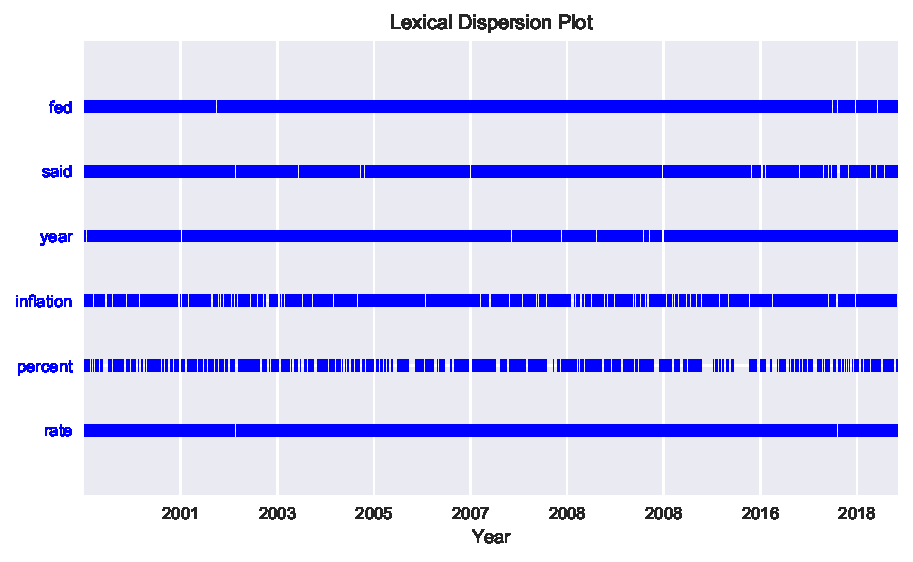
\includegraphics[scale=1]{Images/dispersionplot_topicPLSAorig.pdf}
	\label{dispersionPLSAorig}
\end{figure}

The text data collection comprises between 14 to 97 articles for every policy day. The words of each article are partitioned between the two topics, resulting in a topic coverage probability that indicates to what extent an article is to be attributed to a certain topic. To classify a policy day as belonging either to narrative one ($N_1$) or narrative two ($N_2$), I average the topic coverage probabilities of all articles on a given policy day and attribute the day to the topic that dominates the articles. Figure \ref{classPLSA} in Appendix \ref{AppendixC} depicts the resulting classification of the policy days. 

39 policy days have been attributed to topic 2 and only 17 days to topic 1. Also, quite often both topics command a large share of the articles on a given day, one topic dominating the other only by a small margin. Thus, the classification of the policy days is not as clear cut as one might wish. If we consider how the individual articles have been classified, we would expect that on a given day all articles are attributed to the same topic. That would be a clear indication that a specific narrative, as identified by our topic model, permeated the press reporting at that time. However, as Figure \ref{classdoc01} and \ref{classdoc02} show, quite often the articles on a specific day are almost evenly split between the topics.  
Thus, it stands to reason that the PLSA model without background distribution was not able to infer topics that would separate the policy days in a meaningful manner.

\subsection{Application of PLSA with Background Topic}\label{Ch:implembg}

To improve the topics inferred by PLSA, I introduce a background topic that captures the most common words in the text data. The background topic is a unigram language model generated from the entire text data collection. Thus, every word has been given a probability weight that corresponds to its relative frequency in the collection (see Eq. \ref{estul}). Table \ref{tab:bgtopic} lists the 20 top words of the background topic. 

\begin{table}[h] % Add the following just after the closing bracket on this line to specify a position for the table on the page: [h], [t], [b] or [p] - these mean: here, top, bottom and on a separate page, respectively
	\centering % Centres the table on the page, comment out to left-justify
	\begin{tabular}{ p{3cm}  p{2cm}  p{3cm}  p{2cm} } % The final bracket specifies the number of columns in the table along with left and right borders which are specified using vertical pipes (|); each column can be left, right or center-justified using l, r or c. Columns will widen to hold the content in them by default, to specify a precise width, use p{width}, e.g. p{5cm}
		\toprule % Top horizontal line
		\multicolumn{4}{ c }{Background Topic} \\
		\midrule % In-table horizontal line
		word & prob & word & prob \\
		\midrule
		 fed		& .016 & 	federal reserve	 & .005 \\
		 said		& .013 & 	cut			  	& .005\\
		 year		& .008 & 	interest rate	 & .004\\
		 rate 		& .007 & 	interest rates	 & .004\\
		 percent 	& .007 & 	bank		 	& .004\\
		economy 	& .007 & 	economic		 & .004\\
		inflation 	& .006 & 	expected		 & .004\\
		market 		& .006 & 	markets			 &  .003\\
		rates 		& .006 & 	dollar			 & .003\\
		would 		& .005 & 	could			 & .003\\
		\bottomrule % Bottom horizontal line
	\end{tabular}
	\caption{The background topic $\theta_B$ introduced in PLSA.} % Table caption, can be commented out if no caption is required
	\label{tab:bgtopic} % A label for referencing this table elsewhere, references are used in text as \ref{label}
\end{table}

The most common word in the background topic is \textit{fed}, followed by \textit{said}, \textit{year}, and \textit{rate}. These words also feature prominently in the inferred topics of PLSA without a background distribution. Including the background topic should liberate the learned topics so that meaningful topics can be inferred. To that end, I also need to specify how many words are generated by the background topic (as indicated by the parameter $\lambda_B$). Since this quantity is unknown, I run the model several times with different specifications for $\lambda_B$. The model specifications are as presented in Table \ref{tab:specs2}.

\begin{table}[h] % Add the following just after the closing bracket on this line to specify a position for the table on the page: [h], [t], [b] or [p] - these mean: here, top, bottom and on a separate page, respectively
	\centering % Centres the table on the page, comment out to left-justify
	\begin{tabular}{ l  l  } % The final bracket specifies the number of columns in the table along with left and right borders which are specified using vertical pipes (|); each column can be left, right or center-justified using l, r or c. Columns will widen to hold the content in them by default, to specify a precise width, use p{width}, e.g. p{5cm}
		\toprule % Top horizontal line
		\multicolumn{2}{ c }{Input} \\
		\midrule % In-table horizontal line
		\tabitem A collection of 2'318  text documents & $C=\{d_1,...,d_{2318}\}$ \\
		\tabitem Number of topics & $k = 2$ \\
		\tabitem The background topic & $\theta_B$ \\
		\tabitem Fraction of words generated by $\theta_B$ & $\lambda_B \in [0.1,0.2,0.3,0.4,0.5,0.6,0.7,0.8,0.9]$ \\
		\midrule
		\multicolumn{2}{ c }{Output} \\
		\midrule
		\tabitem Coverage of topics in each document $d_i$ & $\{\pi_{i1}, \pi_{i2}\}$, with $\pi_{i1}+\pi_{i2}=1$\\
		\tabitem $2$ topics & $\{\theta_1, \theta_2\}$\\ %, with $\underset{w \in V}{\sum} \ p(w | \theta_i) = 1$\\
		\bottomrule % Bottom horizontal line
	\end{tabular}
	\caption{Specification of PLSA model with background topic.} % Table caption, can be commented out if no caption is required
	\label{tab:specs2} % A label for referencing this table elsewhere, references are used in text as \ref{label}
\end{table}

The top 20 words of every topic are listed in Tables \ref{tab:topics}--\ref{tab:topics3} in Appendix \ref{AppendixC}. The higher $\lambda_B$, the more the count of common words in the topics decreases in favor of more interesting words. Topic 1 appears to focus on \textit{investing}: With an increasing $\lambda_B$, terms like \textit{investors}, \textit{yield}, \textit{rose}, \textit{fell}, \textit{trading}, \textit{index}, and \textit{stocks} climb to the top of the word distribution. Topic 2, on the other hand, seems to focus on the Fed's \textit{economic analysis}:  With an increasing $\lambda_B$, terms like \textit{economic}, \textit{growth}, \textit{greenspan}, \textit{bernanke}, \textit{statement}, \textit{chairman}, and \textit{economists} come to dominate the topic. Thus, the topics clearly pick up on different subjects (or narratives) in the articles and with an increased use of the background topic, the topical focus of the word distributions becomes salient.

Figure \ref{classPLSAL01} in Appendix \ref{AppendixC} depicts the resulting classification of the policy days for $\lambda_B=0.1$ and Figure \ref{classPLSAL09} for $\lambda_B=0.9$. With $\lambda_B=0.1$, XX policy days have been attributed to topic 2 and only XX days to topic 1. With  $\lambda_B=0.9$,  XX policy days have been attributed to topic 2 and only XX days to topic 1. The introduction of a background model as well as the level of $\lambda_B$ has very little impact on the classification of the policy days. As Figures \ref{classdoc01L01}--\ref{classdoc02L01} and \ref{classdoc01L09}--\ref{classdoc02L09} show, the higher $\lambda_B$, the less ambiguous is the classification of single documents. This is hardly surprising: When $\lambda_B=0.9$, only 10\% of the tokens of a document are still split between topic 1 and 2, which will more commonly lead to an allocation of all tokens to the same topic.


There are several possible approaches to evaluate topic models and their specifications. First, a test can be set up in which a human judge must assess topic quality, in particular the coherence of the inferred topics. Second, traditional metrics, such as log-likelihood of the held-out data, can be employed to measure how well a topic model generalizes. However, such metrics are often negatively correlated with topic quality as assessed by human judges. A third approach is downstream task improvement: A model is assessed based on the statistically significant improvement it brings to another task \cite[~pp.383--384]{Zhai.2016}.

For the purpose of this thesis, we have already outlined how an increase in $\lambda_B$ makes the topics more interpretable. In Chapter \ref{Ch:results} I will also consider how the different topic model specifications affect the downstream task of the financial analysis. 

%\section{NOTES}
%Besprechung - 24.09.2018
%------------------------
%
%- Frage Juan Pablo Ortega ob er Korreferent sein will
%- nur zwei Narrative finden, ohne Daten vorgeben (Texte nach Meeting verwenden, weil sonst ja nicht Interpretation gefunden wird), dann schauen geht die Kurve beim einten Narrativ hoch beim anderen runter
%- es sollten auch die non-target rate sdjustments verwendet werden, weil ansonsten j schon eine Selektion stattfindet - ABER: stimmt das wirklich, weil wenn kein adjustment, dann bewegt sich doch die Kurve nur gemäss neue Infos auf dem Markt, - also vielleicht doch besser keine adjustment heisst non-policy day?
%
%- Example: nach nine eleven gab es tatsächlich ein paar unangemeldetet meetings und daher komische effekte weil wirklich überraschende Verschiebungen in der interest rate
%
%- modell ist gut, unsupervised learning verwenden, nicht vorher sagen, wo geht's hoch und wo runter, und dann ev. auch out-of sample probieren, aber das wäre Paradedisplizin, keine Garantie, dass das funktoniert
%
%---my thoughts before meeting
%
%all absolute Fed target rate changes during the sample period -- ev. sind 10 Jahre nicht genug, vor allem weil es dann nur die extraordinary years sind - 20 Jahre? training and testing samples? aber dann müsste man annehmen, dass die Narrative über die Jahre gleichbleiben? oder aber man nimmt einzelne Datenpunkte aus dem sample raus? einzelne Tage (wohl zu wenige Observations) - einzelne ARtikel - sagt das was aus?


\chapter{Results}\label{Ch:results}

\section{Classification of Policy Days}

Following \cite{Ellingsen.2003}, a day on which the target rate has been adjusted by the Fed is considered a policy day. If the FOMC held a meeting but failed to change the target rate, the day is considered a non-policy day. In this thesis, a 20-year period from October 1998 to October 2018 is analyzed. During this time frame, there are 56 policy days and 5'161 non-policy days. 

Analogously to \citet[pp. 14 -- 15]{Ellingsen.2003}, we take a look at the behavior of the interest rates. Figure \ref{Change01} plots the change in the 3-month rate against the change in the 10-year rate on the policy days. \citet[p. 14]{Ellingsen.2003} found a clear positive relationship between the change of the 10-year and the 3-month rate, with some outliers. Similarly, Figure \ref{Change01} shows a predominantly positive relationship, barring some odd observations, and a concentration around the origin. This indicates that the long-term rates tend to move in the same direction as the short term rates and the target rate change. 

\begin{figure}
	\caption{Response of the 10-year interest rate to a change in the 3-month rate on policy days.}
	\centering
	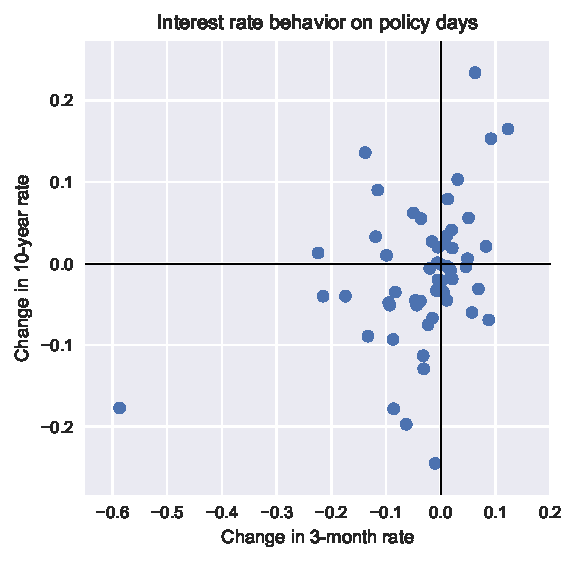
\includegraphics[scale=1]{Images/ChangePlot01.pdf}
	\label{Change01}
\end{figure}

In Figures \ref{Change02} and \ref{Change03}, the policy days are split up according to their classification by either Narrative one or Narrative two (as classified by PLSA without background topic, that is for $\lambda_B=0$). A successful classification of policy days is expected to separate the days characterized by a co-movement of the yield curves from the days on which the rates move in opposite directions. As such, one figure should show a clear positive relationship, with the data points populating quadrants 1 and 3, while the other figure should display a negative relationship, with all data points populating quadrant 2 and 4. However, Figures \ref{Change02} and \ref{Change03} show a rather ambiguous picture. Both figures capture policy days co-movement of the rates as well as days with counter-movement.  It should be noted that \citet[pp. 14--15]{Ellingsen.2003}, too, only found an ambiguous relationship.

\begin{figure}
	\caption{Response of the 10-year interest rate to a change in the 3-month rate on policy days influenced by Narrative one ($\lambda_B=0$).}
	\centering
	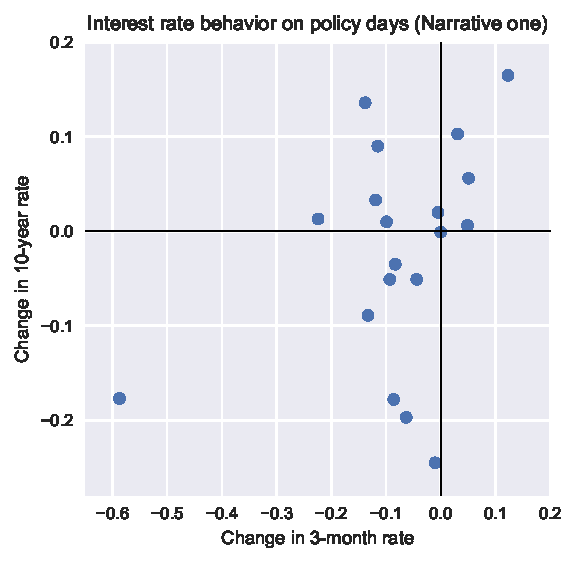
\includegraphics[scale=1]{Images/ChangePlot02.pdf}
	\label{Change02}
\end{figure}

\begin{figure}
	\caption{Response of the 10-year interest rate to a change in the 3-month rate on policy days influenced by Narrative two ($\lambda_B=0$).}
	\centering
	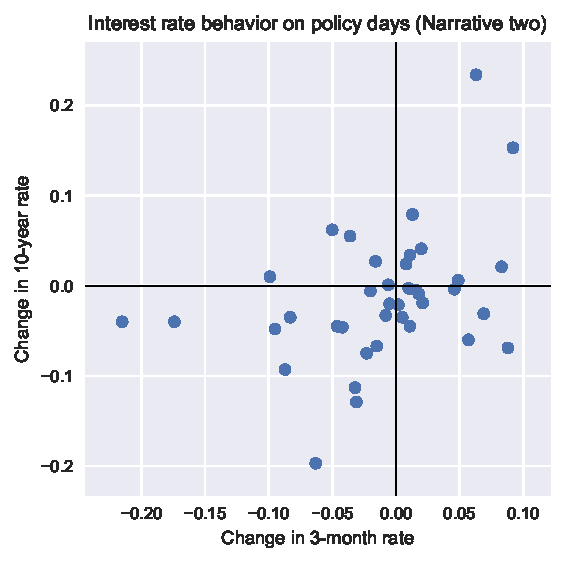
\includegraphics[scale=1]{Images/ChangePlot03.pdf}
	\label{Change03}
\end{figure}

Figures \ref{Change02_L01}--\ref{Change03_L09} in Appendix \ref{AppendixD} show the split of the policy days when $\lambda_B$ is increased to 0.1 and 0.9, respectively. Even though the output of the topic model changes notably in terms of topic quality with an increase in $\lambda_B$, the introduction of a background topic has little impact on the classification of policy days. As such, Figures Figures \ref{Change02_L01}--\ref{Change03_L09} present almost the same picture as Figures \ref{Change02} and \ref{Change03}.
 
\section{Regression Results}
In a next step, I run the regression formulated in Eq. \ref{reg2}. Tables \ref{tab:reg1}--\ref{tab:reg2} give an overview of the regression output depending on the level of $\lambda_B$. Heteroskedasticity robust White’s (1980) standard errors are listed in brackets.  

\begin{table}[h] % Add the following just after the closing bracket on this line to specify a position for the table on the page: [h], [t], [b] or [p] - these mean: here, top, bottom and on a separate page, respectively
	\centering % Centres the table on the page, comment out to left-justify
	\begin{tabular}{ p{2cm}  p{1cm} p{1cm} p{1cm} p{1cm} p{1cm} p{1cm} p{1cm} } % The final bracket specifies the number of columns in the table along with left and right borders which are specified using vertical pipes (|); each column can be left, right or center-justified using l, r or c. Columns will widen to hold the content in them by default, to specify a precise width, use p{width}, e.g. p{5cm}
		\toprule % Top horizontal line
		& 6m & 1y & 3y & 5y & 10y & 20y & 30y \\
		\midrule % In-table horizontal line
		$\alpha_n$ & -0.00 & -0.00 & -0.00 & -0.00 & -0.00 & -0.00 & -0.00\\
		& 0.00 & 0.00 & 0.00 & 0.00 & 0.00 & 0.00 & 0.00\\
		$\beta_n^{NP}$ & 0.36** & 0.30** & 0.28** & 0.25** & 0.18** & 0.13** & 0.12**\\
		& 0.05 & 0.04 & 0.04 & 0.03 & 0.03 & 0.02 & 0.02\\
		$\beta_n^{N1}$ & 0.67** & 0.58** & 0.40** & 0.45** & 0.28** & 0.04 & 0.17**\\
		& 0.07 & 0.08 & 0.10 & 0.11 & 0.08 & 0.09 & 0.06\\
		$\beta_n^{N2}$ & 0.54** & 0.34* & 0.51* & 0.37 & 0.41* & 0.23 & 0.30\\
		& 0.15 & 0.17 & 0.25 & 0.30 & 0.17 & 0.12 & 0.17\\
		$R^2$ & 0.30 & 0.20 & 0.08 & 0.05 & 0.03 & 0.02 & 0.02\\
		$\beta_n^{N1} = \beta_n^{N2}$ & 0.13 & 0.24 & -0.11 & 0.08 & -0.13 & -0.19 & -0.14\\
		\bottomrule % Bottom horizontal line
	\end{tabular}
	\caption{Regression results (classification with $\lambda_B=0$).} % Table caption, can be commented out if no caption is required
	\label{tab:reg1} % A label for referencing this table elsewhere, references are used in text as \ref{label}
\end{table}

\begin{table}[h] % Add the following just after the closing bracket on this line to specify a position for the table on the page: [h], [t], [b] or [p] - these mean: here, top, bottom and on a separate page, respectively
	\centering % Centres the table on the page, comment out to left-justify
	\begin{tabular}{ p{2cm}  p{1cm} p{1cm} p{1cm} p{1cm} p{1cm} p{1cm} p{1cm} } % The final bracket specifies the number of columns in the table along with left and right borders which are specified using vertical pipes (|); each column can be left, right or center-justified using l, r or c. Columns will widen to hold the content in them by default, to specify a precise width, use p{width}, e.g. p{5cm}
		\toprule % Top horizontal line
						& 6m 		& 1y 		& 3y 		& 5y 		& 10y 		& 20y 		& 30y \\
		\midrule % In-table horizontal line
	$\alpha_n$ & -0.00 & -0.00 & -0.00 & -0.00 & -0.00 & -0.00 & -0.00\\
	& 0.00 & 0.00 & 0.00 & 0.00 & 0.00 & 0.00 & 0.00\\
	$\beta_n^{NP}$ & 0.36** & 0.30** & 0.28** & 0.25** & 0.18** & 0.13** & 0.12**\\
	& 0.05 & 0.04 & 0.04 & 0.03 & 0.03 & 0.02 & 0.02\\
	$\beta_n^{N1}$ & 0.67** & 0.58** & 0.41** & 0.46** & 0.29** & 0.05 & 0.17**\\
	& 0.07 & 0.08 & 0.10 & 0.11 & 0.08 & 0.09 & 0.06\\
	$\beta_n^{N2}$ & 0.55** & 0.33* & 0.47* & 0.34 & 0.38* & 0.19 & 0.28\\
	& 0.14 & 0.15 & 0.24 & 0.28 & 0.16 & 0.12 & 0.15\\
	$R^2$ & 0.30 & 0.20 & 0.08 & 0.05 & 0.03 & 0.02 & 0.02\\
	$\beta_n^{N1} = \beta_n^{N2}$ & 0.12 & 0.25 & -0.06 & 0.12 & -0.09 & -0.14 & -0.11\\
		\bottomrule % Bottom horizontal line
	\end{tabular}
	\caption{Regression results (classification with $\lambda_B=0.1$).} % Table caption, can be commented out if no caption is required
	\label{tab:reg2} % A label for referencing this table elsewhere, references are used in text as \ref{label}
\end{table}

\begin{table}[h] % Add the following just after the closing bracket on this line to specify a position for the table on the page: [h], [t], [b] or [p] - these mean: here, top, bottom and on a separate page, respectively
	\centering % Centres the table on the page, comment out to left-justify
	\begin{tabular}{ p{2cm}  p{1cm} p{1cm} p{1cm} p{1cm} p{1cm} p{1cm} p{1cm} } % The final bracket specifies the number of columns in the table along with left and right borders which are specified using vertical pipes (|); each column can be left, right or center-justified using l, r or c. Columns will widen to hold the content in them by default, to specify a precise width, use p{width}, e.g. p{5cm}
		\toprule % Top horizontal line
						& 6m 		& 1y 		& 3y 		& 5y 		& 10y 		& 20y 		& 30y \\
		\midrule % In-table horizontal line
		$\alpha_n$ & -0.00 & -0.00 & -0.00 & -0.00 & -0.00 & -0.00 & -0.00\\
		& 0.00 & 0.00 & 0.00 & 0.00 & 0.00 & 0.00 & 0.00\\
		$\beta_n^{NP}$ & 0.36** & 0.30** & 0.28** & 0.25** & 0.18** & 0.13** & 0.12**\\
		& 0.05 & 0.04 & 0.04 & 0.03 & 0.03 & 0.02 & 0.02\\
		$\beta_n^{N1}$ & 0.69** & 0.58** & 0.41** & 0.46** & 0.29** & 0.05 & 0.18**\\
		& 0.06 & 0.08 & 0.10 & 0.11 & 0.08 & 0.09 & 0.06\\
		$\beta_n^{N2}$ & 0.50** & 0.34* & 0.46* & 0.33 & 0.36* & 0.18 & 0.26\\
		& 0.14 & 0.15 & 0.22 & 0.26 & 0.15 & 0.11 & 0.14\\
		$R^2$ & 0.30 & 0.20 & 0.08 & 0.05 & 0.03 & 0.02 & 0.02\\
		$\beta_n^{N1} = \beta_n^{N2}$ & 0.19 & 0.25 & -0.05 & 0.13 & -0.07 & -0.13 & -0.08\\
		\bottomrule % Bottom horizontal line
	\end{tabular}
	\caption{Regression results (classification with $\lambda_B=0.9$).} % Table caption, can be commented out if no caption is required
	\label{tab:reg3} % A label for referencing this table elsewhere, references are used in text as \ref{label}
\end{table}

\begin{figure}
	\caption{Regression coefficients for narrative one and two without background topic.}
	\centering
	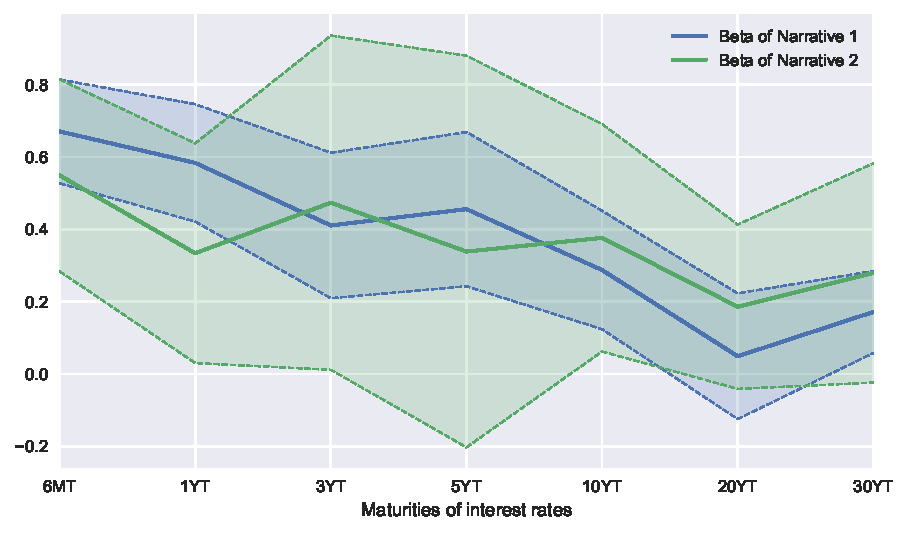
\includegraphics[scale=1]{Images/betasLamb0_0.pdf}
	\label{betaL00}
\end{figure}

\begin{figure}
	\caption{Regression coefficients for narrative one and two with $\lambda_B=0.1$.}
	\centering
	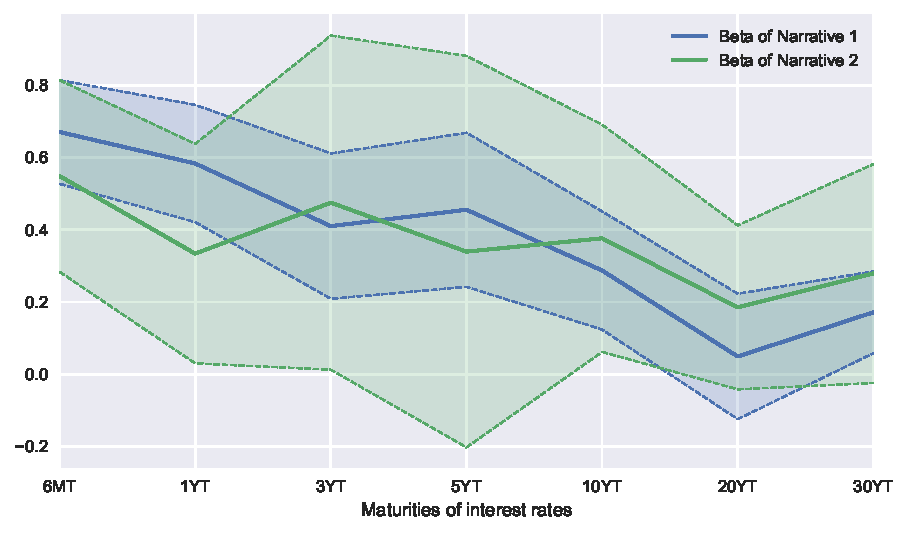
\includegraphics[scale=1]{Images/betasLamb0_1.pdf}
	\label{betaL01}
\end{figure}

\begin{figure}
	\caption{Regression coefficients for narrative one and two with $\lambda_B=0.9$.}
	\centering
	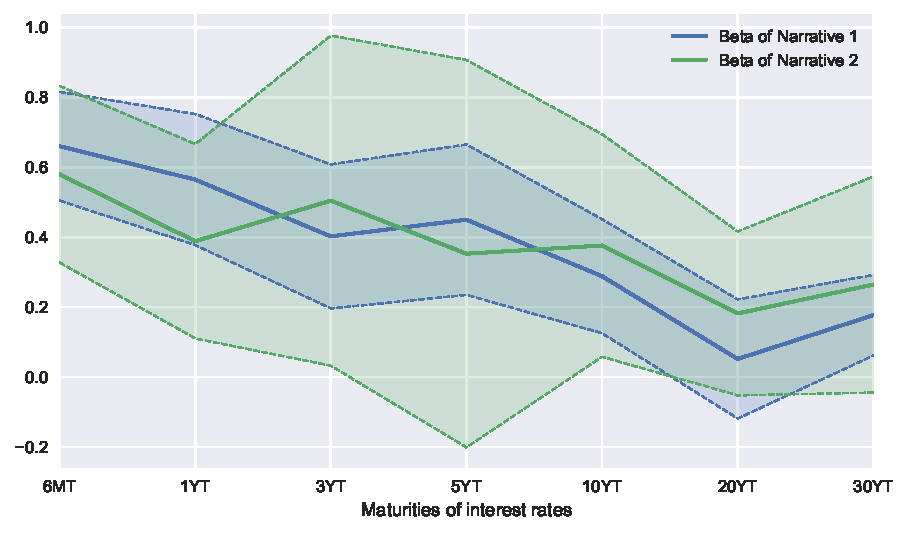
\includegraphics[scale=1]{Images/betasLamb0_9.pdf}
	\label{betaL09}
\end{figure}

\textcolor{red}{note that classification remains very stable across lambdas}
\textcolor{red}{equality test, the difference in betas is never significant!}

\begin{figure}
	\caption{Boxplot showing the weight or narrative one (without background topic) on policy days classified as endogenous or exogenous by \citet[p. 11]{Ellingsen.2003}.}
	\centering
	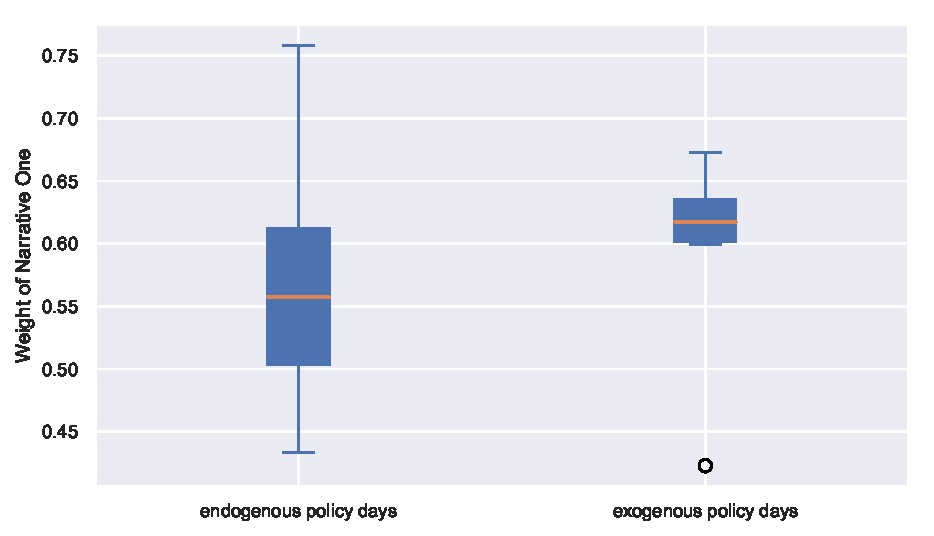
\includegraphics[scale=1]{Images/boxplot_orig.pdf}
	\label{boxplotL00}
\end{figure}

\begin{figure}
	\caption{Boxplot showing the weight or narrative one (with $\lambda_B=0.1$) on policy days classified as endogenous or exogenous by \citet[p. 11]{Ellingsen.2003}.}
	\centering
	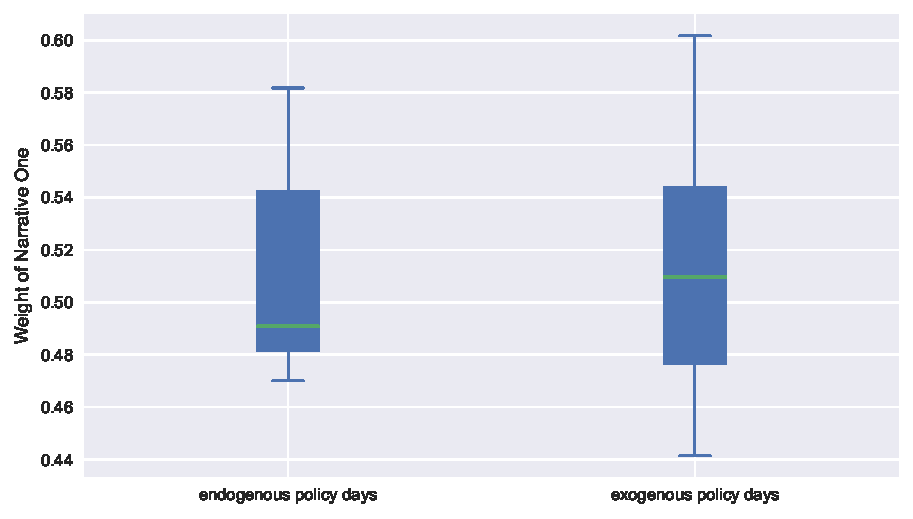
\includegraphics[scale=1]{Images/boxplot_Lamb_0_1.pdf}
	\label{boxplotL01}
\end{figure}

\begin{figure}
	\caption{Boxplot showing the weight or narrative one (with $\lambda_B=0.9$) on policy days classified as endogenous or exogenous by \citet[p. 11]{Ellingsen.2003}.}
	\centering
	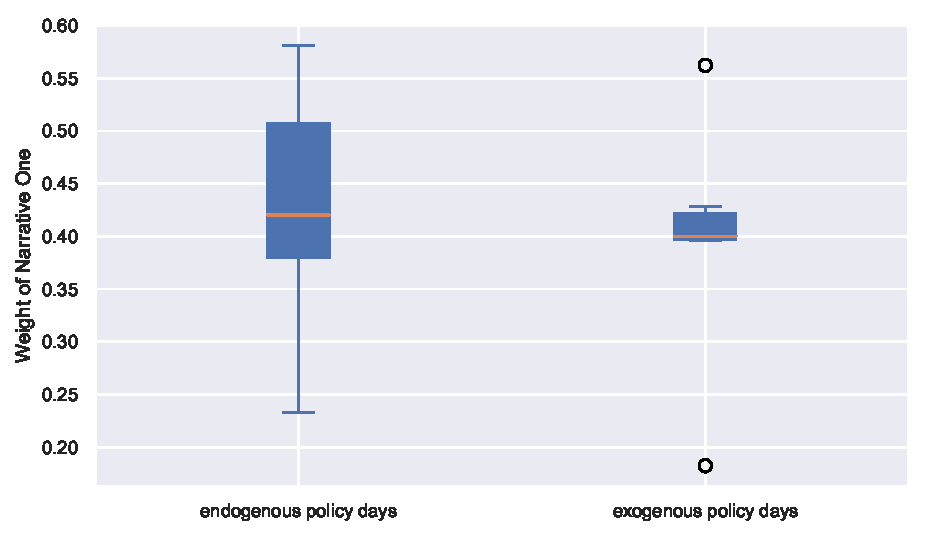
\includegraphics[scale=1]{Images/boxplot_Lamb_0_9.pdf}
	\label{boxplotL09}
\end{figure}

%\begin{table}[h] % Add the following just after the closing bracket on this line to specify a position for the table on the page: [h], [t], [b] or [p] - these mean: here, top, bottom and on a separate page, respectively
%	\centering % Centres the table on the page, comment out to left-justify
%	\begin{tabular}{ p{2cm}  p{1cm} p{1cm} p{1cm} p{1cm} p{1cm} p{1cm} p{1cm} } % The final bracket specifies the number of columns in the table along with left and right borders which are specified using vertical pipes (|); each column can be left, right or center-justified using l, r or c. Columns will widen to hold the content in them by default, to specify a precise width, use p{width}, e.g. p{5cm}
%		\toprule % Top horizontal line
%		& 6m 		& 1y 		& 3y 		& 5y 		& 10y 		& 20y 		& 30y \\
%		\midrule % In-table horizontal line
%		$\alpha_n$		& -0.00 	& -0.00 	& -0.00 	& -0.00  	& -0.00 	& -0.00 	& -0.00    \\
%		& (0.00) 	& (0.00)  	& (0.00)  	& (0.00) 	& (0.00) 	& (0.00) 	&  (0.00)   \\
%		$\beta_n^{NP}$	&  			&    		&  			&  			&  			&  			&   \\
%		& 			&  			&  			&  			&   		&  			&     \\
%		$\beta_n^{N1}$	&  			&  			&    		&  			&  			& 			&   \\
%		&  			&  			&  			&  			&   		&  			&    \\
%		$\beta_n^{N2}$	&  			&    		&  			&  			&  			& 			& \\
%		& 			&  			&  			&  			& 			& 			&    \\
%		$R^2$			&  			&  			&  			&  			&  			&  			&     \\
%		
%		\bottomrule % Bottom horizontal line
%	\end{tabular}
%	\caption{Regression results (applying classification without background topic).} % Table caption, can be commented out if no caption is required
%	\label{tab:reg1} % A label for referencing this table elsewhere, references are used in text as \ref{label}
%\end{table}

\section{Comparison to Ellingesen et al.}
put boxplot that Gruber wanted somewhere

\chapter{Discussion}

\chapter{Conclusion}


\newpage

\phantomsection 
\addcontentsline{toc}{chapter}{References} 
%\renewcommand\bibname{References}

\bibliography{EconomicNarrative}



\newpage

\appendix
\noappendicestocpagenum
\addappheadtotoc
%%\appendixpage



\renewcommand{\theequation}{A.\arabic{equation}}


\chapter{Target Rate and Yield Curves}\label{AppendixA}
\vspace{-0.5cm}
%\lipsum[2-4]

\begin{table}[h] % Add the following just after the closing bracket on this line to specify a position for the table on the page: [h], [t], [b] or [p] - these mean: here, top, bottom and on a separate page, respectively
	\centering % Centres the table on the page, comment out to left-justify
	\begin{tabular}{r r r r r r r } % The final bracket specifies the number of columns in the table along with left and right borders which are specified using vertical pipes (|); each column can be left, right or center-justified using l, r or c. Columns will widen to hold the content in them by default, to specify a precise width, use p{width}, e.g. p{5cm}
		\toprule % Top horizontal line
%		& & & & & \multicolumn{2}{l}{FOMC Meeting on} & & & & & & \multicolumn{2}{l}{FOMC Meeting on} \\ % Amalgamating several columns into one cell is done using the \multicolumn command with the number of columns to amalgamate as the first argument and then the justification (l, r or c)
		%		\cmidrule(l){6-7} % Horizontal line spanning less than the full width of the table - you can add (r) or (l) just before the opening curly bracket to shorten the rule on the left or right side
%		Date & $Tgt_{low}$ & $Tgt_{up}$ & $\Delta Tgt_{low}$ & $\Delta Tgt_{up}$ & day prior &  same day & Date & $Tgt_{low}$ & $Tgt_{up}$ & $\Delta Tgt_{low}$ & $\Delta Tgt_{up}$ & day prior &  same day \\ % Column names row
		\multicolumn{7}{c}{Dates of all FOMC meetings since January 1, 1998} \\
		\midrule % In-table horizontal line
						26.09.2018 & 18.03.2015 & 13.12.2011 & *07.02.2009 & 12.12.2006 & 12.08.2003 & 31.01.2001 \\
						01.08.2018 & 28.01.2015 & *28.11.2011 & 28.01.2009 & 25.10.2006 & 25.06.2003 & *03.01.2001 \\
						13.06.2018 & 17.12.2014 & 02.11.2011 & *16.01.2009 & 20.09.2006 & 06.05.2003 & 19.12.2000 \\
						02.05.2018 & 29.10.2014 & 21.09.2011 & 16.12.2008 & 08.08.2006 & *16.04.2003 & 15.11.2000 \\
						21.03.2018 & 17.09.2014 & 09.08.2011 & 29.10.2008 & 29.06.2006 & *08.04.2003 & 03.10.2000 \\
						31.01.2018 & 30.07.2014 & *01.08.2011 & *07.10.2008 & 10.05.2006 & *01.04.2003 & 22.08.2000 \\
						13.12.2017 & 18.06.2014 & 22.06.2011 & *29.09.2008 & 28.03.2006 & *25.03.2003 & 28.06.2000 \\
						01.11.2017 & 30.04.2014 & 27.04.2011 & 16.09.2008 & 31.01.2006 & 18.03.2003 & 16.05.2000 \\
						20.09.2017 & 19.03.2014 & 15.03.2011 & 05.08.2008 & 13.12.2005 & 29.01.2003 & 21.03.2000 \\
						26.07.2017 & *04.03.2014 & 26.01.2011 & *24.07.2008 & 01.11.2005 & 10.12.2002 & 02.02.2000 \\
						14.06.2017 & 29.01.2014 & 14.12.2010 & 25.06.2008 & 20.09.2005 & 06.11.2002 & 21.12.1999 \\
						03.05.2017 & 18.12.2013 & 03.11.2010 & 30.04.2008 & 09.08.2005 & 24.09.2002 & 16.11.1999 \\
						15.03.2017 & 30.10.2013 & *15.10.2010 & 18.03.2008 & 30.06.2005 & 13.08.2002 & 05.10.1999 \\
						01.02.2017 & *16.10.2013 & 21.09.2010 & *10.03.2008 & 03.05.2005 & 26.06.2002 & 24.08.1999 \\
						14.12.2016 & 18.09.2013 & 10.08.2010 & 30.01.2008 & 22.03.2005 & 07.05.2002 & 30.06.1999 \\
						02.11.2016 & 31.07.2013 & 23.06.2010 & *21.01.2008 & 02.02.2005 & 19.03.2002 & 18.05.1999 \\
						21.09.2016 & 19.06.2013 & *09.05.2010 & *09.01.2008 & 14.12.2004 & 30.01.2002 & 30.03.1999 \\
						27.07.2016 & 01.05.2013 & 28.04.2010 & 11.12.2007 & 10.11.2004 & 11.12.2001 & 03.02.1999 \\
						15.06.2016 & 20.03.2013 & 16.03.2010 & *06.12.2007 & 21.09.2004 & 06.11.2001 & 22.12.1998 \\
						27.04.2016 & 30.01.2013 & 27.01.2010 & 31.10.2007 & 10.08.2004 & 02.10.2001 & 17.11.1998 \\
						16.03.2016 & 12.12.2012 & 16.12.2009 & 18.09.2007 & 30.06.2004 & *17.09.2001 & *15.10.1998 \\
						27.01.2016 & 24.10.2012 & 04.11.2009 & *16.08.2007 & 04.05.2004 & *13.09.2001 & 29.09.1998 \\
						16.12.2015 & 13.09.2012 & 23.09.2009 & *10.08.2007 & 16.03.2004 & 21.08.2001 & *21.09.1998 \\
						28.10.2015 & 01.08.2012 & 12.08.2009 & 07.08.2007 & 28.01.2004 & 27.06.2001 & 18.08.1998 \\
						17.09.2015 & 20.06.2012 & 24.06.2009 & 28.06.2007 & 09.12.2003 & 15.05.2001 & 01.07.1998 \\
						29.07.2015 & 25.04.2012 & *03.06.2009 & 09.05.2007 & 28.10.2003 & *18.04.2001 & 19.05.1998 \\
						17.06.2015 & 13.03.2012 & 29.04.2009 & 21.03.2007 & 16.09.2003 & *11.04.2001 & 31.03.1998 \\
						29.04.2015 & 25.01.2012 & 18.03.2009 & 31.01.2007 &  & 20.03.2001 & 04.02.1998 \\
						\midrule																
						\multicolumn{6}{l}{* indicates an unscheduled meeting/conference call} & \\
		%		\midrule % In-table horizontal line
		%		Average Rate & 0.920 & 0.882 & 0.477 & 0.539 & 0.923\\ % Summary/total row
		\bottomrule % Bottom horizontal line
	\end{tabular}
	\caption{FOMC meetings.} % Table caption, can be commented out if no caption is required
	\label{tab:meetings} % A label for referencing this table elsewhere, references are used in text as \ref{label}
\end{table}




\newpage
\thispagestyle{empty}

\begin{sidewaystable} % Add the following just after the closing bracket on this line to specify a position for the table on the page: [h], [t], [b] or [p] - these mean: here, top, bottom and on a separate page, respectively
	\centering % Centres the table on the page, comment out to left-justify
	\begin{tabular}{r r r r r c c | r r r r r c c } % The final bracket specifies the number of columns in the table along with left and right borders which are specified using vertical pipes (|); each column can be left, right or center-justified using l, r or c. Columns will widen to hold the content in them by default, to specify a precise width, use p{width}, e.g. p{5cm}
		\toprule % Top horizontal line
		& & & & & \multicolumn{2}{l}{FOMC Meeting on} & & & & & & \multicolumn{2}{l}{FOMC Meeting on} \\ % Amalgamating several columns into one cell is done using the \multicolumn command with the number of columns to amalgamate as the first argument and then the justification (l, r or c)
		%		\cmidrule(l){6-7} % Horizontal line spanning less than the full width of the table - you can add (r) or (l) just before the opening curly bracket to shorten the rule on the left or right side
		Date & $Tgt_{low}$ & $Tgt_{up}$ & $\Delta Tgt_{low}$ & $\Delta Tgt_{up}$ & day prior &  same day & Date & $Tgt_{low}$ & $Tgt_{up}$ & $\Delta Tgt_{low}$ & $\Delta Tgt_{up}$ & day prior &  same day \\ % Column names row
		\midrule % In-table horizontal line
		27.09.2018 & 2.00\% & 2.25\% & 25  &  -   & 1 & 0 & 14.12.2004 & 2.25\% &  - & 25  &  - & 0 & 1 \\
		14.06.2018 & 1.75\% & 2.00\% & 25  &  -   & 1 & 0 & 10.11.2004 & 2.00\% &  - & 25  &  - & 0 & 1 \\
		22.03.2018 & 1.50\% & 1.75\% & 25  &  -   & 1 & 0 & 21.09.2004 & 1.75\% &  - & 25  &  - & 0 & 1 \\
		14.12.2017 & 1.25\% & 1.50\% & 25  &  -   & 1 & 0 & 10.08.2004 & 1.50\% &  - & 25  &  - & 0 & 1 \\
		15.06.2017 & 1.00\% & 1.25\% & 25  &  -   & 1 & 0 & 30.06.2004 & 1.25\% &  - & 25  &  - & 0 & 1 \\
		16.03.2017 & 0.75\% & 1.00\% & 25  &  -   & 1 & 0 & \cellcolor{lightgray!25}25.06.2003 & \cellcolor{lightgray!25}1.00\% &  \cellcolor{lightgray!25}- & \cellcolor{lightgray!25}-25 &  \cellcolor{lightgray!25}- & 0 & 1 \\
		15.12.2016 & 0.50\% & 0.75\% & 25  &  -   & 1 & 0 & \cellcolor{lightgray!25}06.11.2002 & \cellcolor{lightgray!25}1.25\% &  \cellcolor{lightgray!25}- & \cellcolor{lightgray!25}-50 &  \cellcolor{lightgray!25}- & 0 & 1 \\
		17.12.2015 & 0.25\% & 0.50\% & 25  &  -   & 1 & 0 & \cellcolor{lightgray!25}11.12.2001 & \cellcolor{lightgray!25}1.75\% &  \cellcolor{lightgray!25}- & \cellcolor{lightgray!25}-25 &  \cellcolor{lightgray!25}- & 0 & 1 \\
		\cellcolor{lightgray!25}16.12.2008 & \cellcolor{lightgray!25}0.00\% & \cellcolor{lightgray!25}0.25\% & \cellcolor{lightgray!25}-75 & \cellcolor{lightgray!25}-100 & 0 & 1 & \cellcolor{lightgray!25}06.11.2001 & \cellcolor{lightgray!25}2.00\% &  \cellcolor{lightgray!25}- & \cellcolor{lightgray!25}-50 &  \cellcolor{lightgray!25}- & 0 & 1 \\
		\cellcolor{lightgray!25}29.10.2008 & \cellcolor{lightgray!25}1.00\% &   \cellcolor{lightgray!25}-    & \cellcolor{lightgray!25}-50 &  \cellcolor{lightgray!25}-   & 0 & 1 & \cellcolor{lightgray!25}02.10.2001 & \cellcolor{lightgray!25}2.50\% &  \cellcolor{lightgray!25}- & \cellcolor{lightgray!25}-50 &  \cellcolor{lightgray!25}- & 0 & 1 \\
		\cellcolor{lightgray!25}*08.10.2008 & \cellcolor{lightgray!25}1.50\% &  \cellcolor{lightgray!25} -    & \cellcolor{lightgray!25}-50 &  \cellcolor{lightgray!25}-   & 1 & 0 & \cellcolor{lightgray!25}*17.09.2001 & \cellcolor{lightgray!25}3.00\% &  \cellcolor{lightgray!25}- & \cellcolor{lightgray!25}-50 &  \cellcolor{lightgray!25}- & 0 & 1 \\
		\cellcolor{lightgray!25}30.04.2008 & \cellcolor{lightgray!25}2.00\% &  \cellcolor{lightgray!25} -    & \cellcolor{lightgray!25}-25 &  \cellcolor{lightgray!25}-   & 0 & 1 & \cellcolor{lightgray!25}21.08.2001 & \cellcolor{lightgray!25}3.50\% &  \cellcolor{lightgray!25}- & \cellcolor{lightgray!25}-25 &  \cellcolor{lightgray!25}- & 0 & 1 \\
		\cellcolor{lightgray!25}18.03.2008 & \cellcolor{lightgray!25}2.25\% &  \cellcolor{lightgray!25} -    & \cellcolor{lightgray!25}-75 &  \cellcolor{lightgray!25}-   & 0 & 1 & \cellcolor{lightgray!25}27.06.2001 & \cellcolor{lightgray!25}3.75\% &  \cellcolor{lightgray!25}- & \cellcolor{lightgray!25}-25 &  \cellcolor{lightgray!25}- & 0 & 1 \\
		\cellcolor{lightgray!25}30.01.2008 & \cellcolor{lightgray!25}3.00\% &  \cellcolor{lightgray!25} -    & \cellcolor{lightgray!25}-50 &  \cellcolor{lightgray!25}-   & 0 & 1 & \cellcolor{lightgray!25}15.05.2001 & \cellcolor{lightgray!25}4.00\% &  \cellcolor{lightgray!25}- & \cellcolor{lightgray!25}-50 &  \cellcolor{lightgray!25}- & 0 & 1 \\
		\cellcolor{lightgray!25}*22.01.2008 & \cellcolor{lightgray!25}3.50\% &  \cellcolor{lightgray!25} -    & \cellcolor{lightgray!25}-75 &  \cellcolor{lightgray!25}-   & 1 & 0 & \cellcolor{lightgray!25}*18.04.2001 & \cellcolor{lightgray!25}4.50\% &  \cellcolor{lightgray!25}- & \cellcolor{lightgray!25}-50 &  \cellcolor{lightgray!25}- & 0 & 1 \\
		\cellcolor{lightgray!25}11.12.2007 & \cellcolor{lightgray!25}4.25\% &  \cellcolor{lightgray!25} -    & \cellcolor{lightgray!25}-25 &  \cellcolor{lightgray!25}-   & 0 & 1 & \cellcolor{lightgray!25}20.03.2001 & \cellcolor{lightgray!25}5.00\% &  \cellcolor{lightgray!25}- & \cellcolor{lightgray!25}-50 &  \cellcolor{lightgray!25}- & 0 & 1 \\
		\cellcolor{lightgray!25}31.10.2007 & \cellcolor{lightgray!25}4.50\% &  \cellcolor{lightgray!25} -    & \cellcolor{lightgray!25}-25 &  \cellcolor{lightgray!25}-   & 0 & 1 & \cellcolor{lightgray!25}31.01.2001 & \cellcolor{lightgray!25}5.50\% &  \cellcolor{lightgray!25}- & \cellcolor{lightgray!25}-50 &  \cellcolor{lightgray!25}- & 0 & 1 \\
		\cellcolor{lightgray!25}18.09.2007 & \cellcolor{lightgray!25}4.75\% &  \cellcolor{lightgray!25} -    & \cellcolor{lightgray!25}-50 &  \cellcolor{lightgray!25}-   & 0 & 1 & \cellcolor{lightgray!25}*03.01.2001 & \cellcolor{lightgray!25}6.00\% &  \cellcolor{lightgray!25}- & \cellcolor{lightgray!25}-50 &  \cellcolor{lightgray!25}- & 0 & 1 \\
		29.06.2006 & 5.25\% &   -    & 25  &  -   & 0 & 1 & 16.05.2000 & 6.50\% &  - & 50  &  - & 0 & 1 \\
		10.05.2006 & 5.00\% &   -    & 25  &  -   & 0 & 1 & 21.03.2000 & 6.00\% &  - & 25  &  - & 0 & 1 \\
		28.03.2006 & 4.75\% &   -    & 25  &  -   & 0 & 1 & 02.02.2000 & 5.75\% &  - & 25  &  - & 0 & 1 \\
		31.01.2006 & 4.50\% &   -    & 25  &  -   & 0 & 1 & 16.11.1999 & 5.50\% &  - & 25  &  - & 0 & 1 \\
		13.12.2005 & 4.25\% &   -    & 25  &  -   & 0 & 1 & 24.08.1999 & 5.25\% &  - & 25  &  - & 0 & 1 \\
		01.11.2005 & 4.00\% &   -    & 25  &  -   & 0 & 1 & 30.06.1999 & 5.00\% &  - & 25  &  - & 0 & 1 \\
		20.09.2005 & 3.75\% &   -    & 25  &  -   & 0 & 1 & \cellcolor{lightgray!25}17.11.1998 & \cellcolor{lightgray!25}4.75\% &  \cellcolor{lightgray!25}- & \cellcolor{lightgray!25}-25 &  \cellcolor{lightgray!25}- & 0 & 1 \\
		09.08.2005 & 3.50\% &   -    & 25  &  -   & 0 & 1 & \cellcolor{lightgray!25}*15.10.1998 & \cellcolor{lightgray!25}5.00\% &  \cellcolor{lightgray!25}- & \cellcolor{lightgray!25}-25 &  \cellcolor{lightgray!25}- & 0 & 1 \\
		30.06.2005 & 3.25\% &   -    & 25  &  -   & 0 & 1 & \cellcolor{lightgray!25}29.09.1998 & \cellcolor{lightgray!25}5.25\% &  \cellcolor{lightgray!25}- & \cellcolor{lightgray!25}-25 &  \cellcolor{lightgray!25}- & 0 & 1 \\
		03.05.2005 & 3.00\% &   -    & 25  &  -   & 0 & 1 &            &      &  &     &  &   &   \\
		22.03.2005 & 2.75\% &   -    & 25  &  -   & 0 & 1 &            &      &  &     &  &   &   \\
		02.02.2005 & 2.50\% &   -    & 25  &  -   & 0 & 1 &            &      &  &     &  &   & \\	
		\midrule																
		\multicolumn{13}{l}{ $\Delta Tgt$ are given in basis points \hspace{1cm}  * indicates a target rate adjustment following an unscheduled meeting} & \\
		%		\midrule % In-table horizontal line
		%		\midrule % In-table horizontal line
		%		Average Rate & 0.920 & 0.882 & 0.477 & 0.539 & 0.923\\ % Summary/total row
		\bottomrule % Bottom horizontal line
	\end{tabular}
	\caption{Target rate adjustments since January 1, 1998.} % Table caption, can be commented out if no caption is required
	\label{tab:target} % A label for referencing this table elsewhere, references are used in text as \ref{label}
\end{sidewaystable}

\newpage
\thispagestyle{firststyle}

\begin{figure}
	\caption{Target rate and treasury yields of all maturities.}
	\centering
	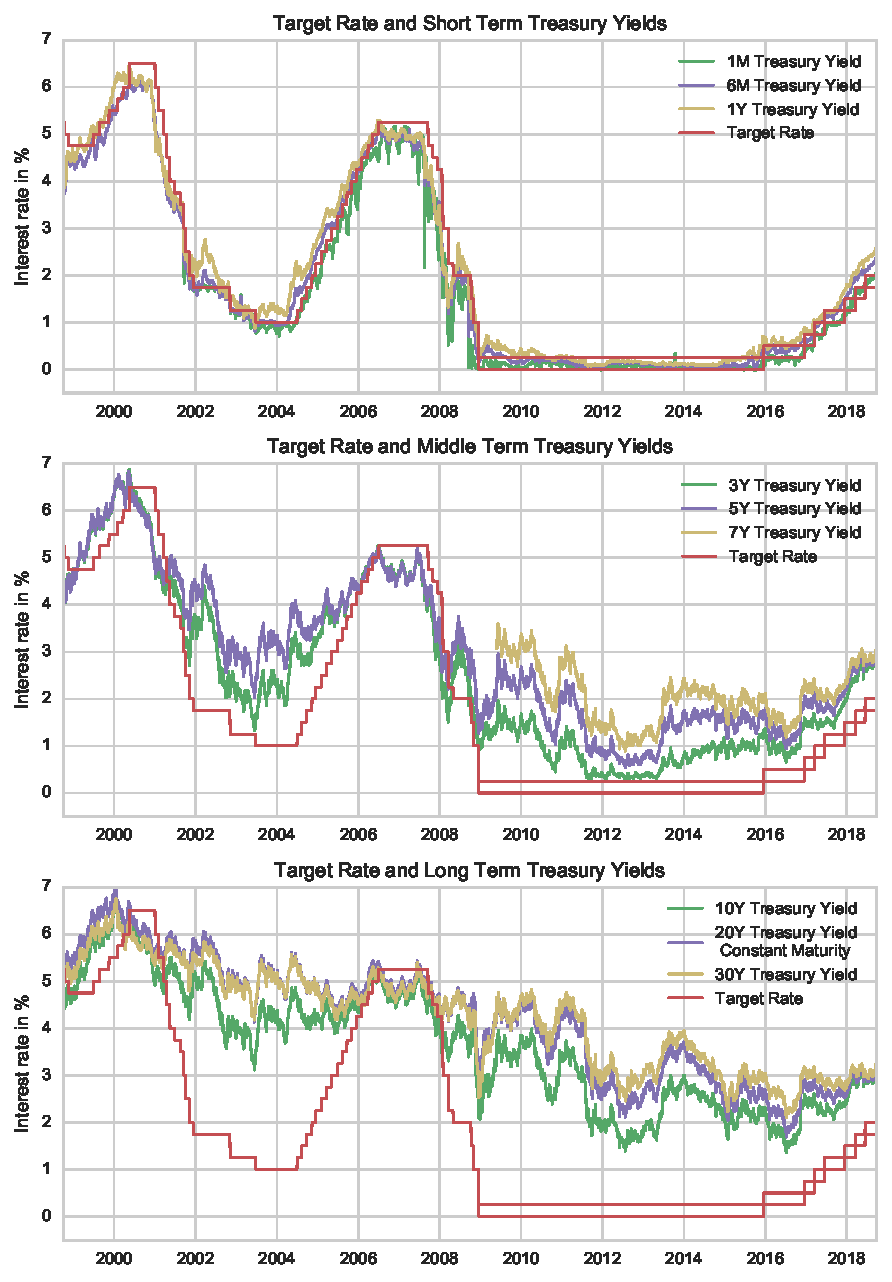
\includegraphics[scale=1]{Images/alltreasury.pdf}
	\label{alltreasury}
\end{figure}


\renewcommand{\theequation}{B.\arabic{equation}}


\chapter{Text Data}\label{AppendixB}

Figure \ref{tokencount} illustrates the distribution of the token and article count of the text data across policy days.
After tokenization, the text data collection encompasses more than 1’600’000 tokens (red bars). After
the removal of stop words, the token count drops to roughly 1’100’000 tokens. Subsequently, the
non-alphabetic characters, especially the punctuations marks, are removed and the final count
amounts to approximately 850’000 tokens (blue bars). Note that the blue bars illustrate the token count after preprocessing
but before feature engineering.



\begin{figure}
	\caption{Token and article count for every policy day.}
	\centering
	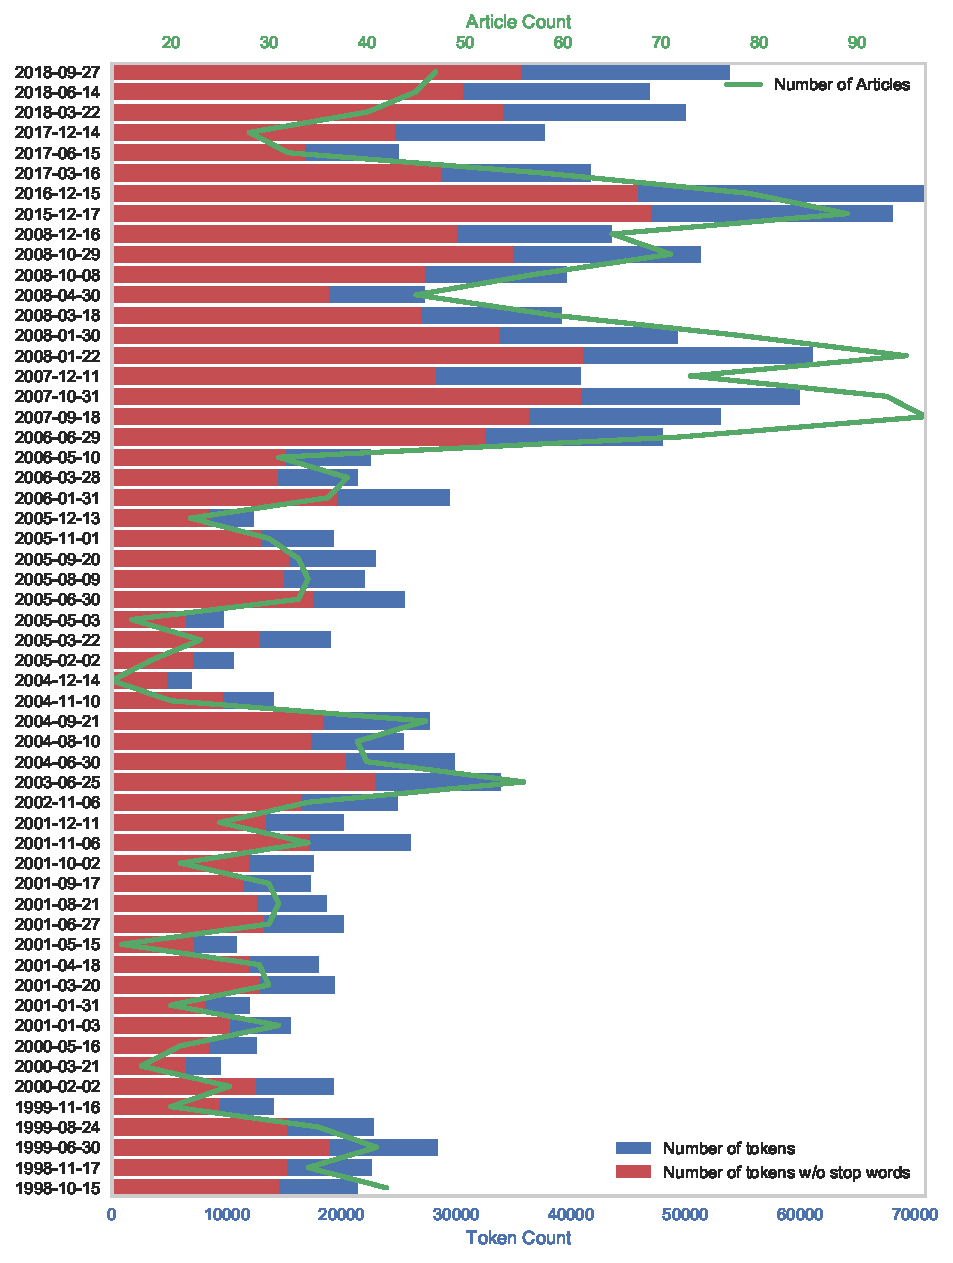
\includegraphics[scale=1]{Images/tokencount.pdf}
	\label{tokencount}
\end{figure}

\renewcommand{\theequation}{C.\arabic{equation}}


\chapter{Topic Model Output}\label{AppendixC}

\section{PLSA without background topic}

\begin{sidewaysfigure}
	\caption{Policy day classification according to original PLSA.}
	\centering
	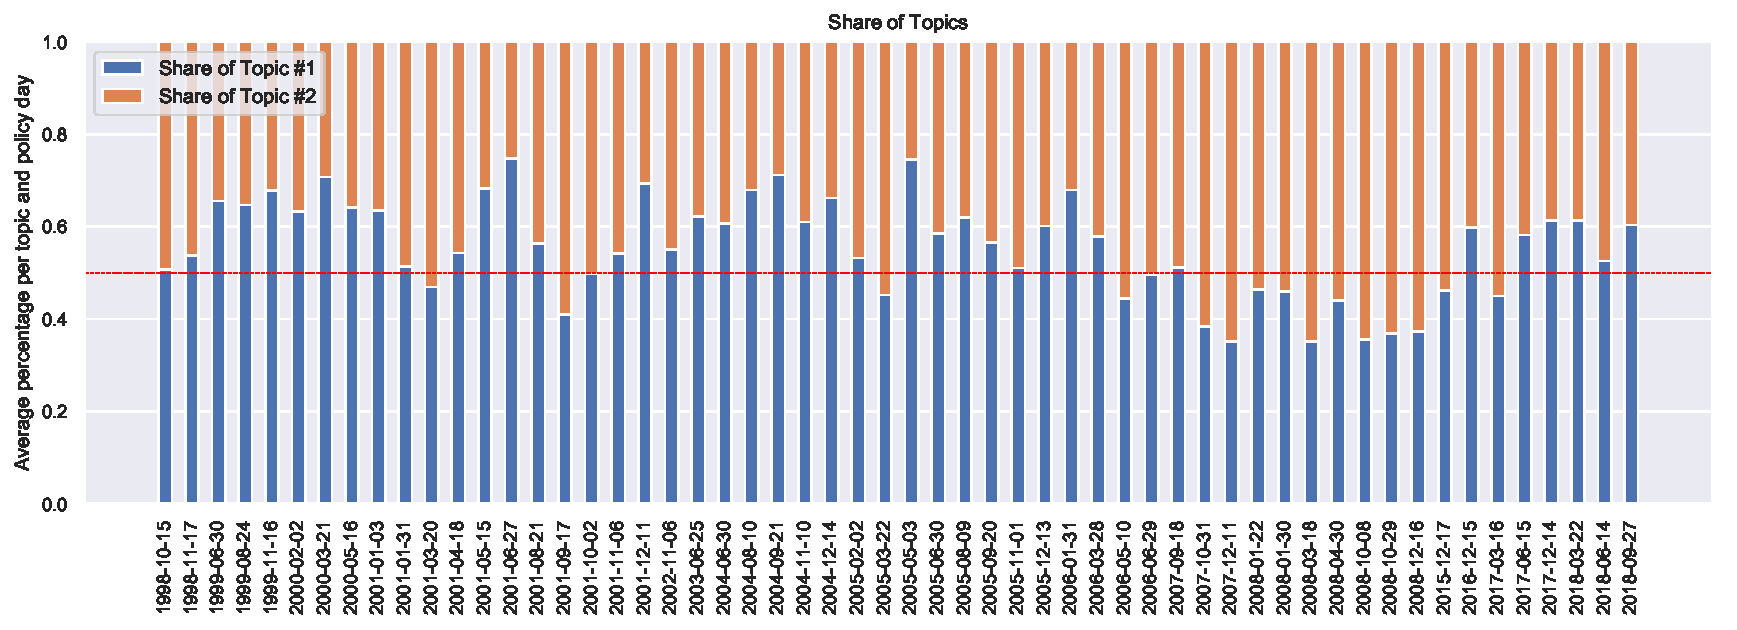
\includegraphics[scale=0.8]{Images/plsamodelling_orig.pdf}
	\label{classPLSA}
\end{sidewaysfigure}

\begin{figure}
	\caption{Document classification according to original PLSA - Part I.}
	\centering
	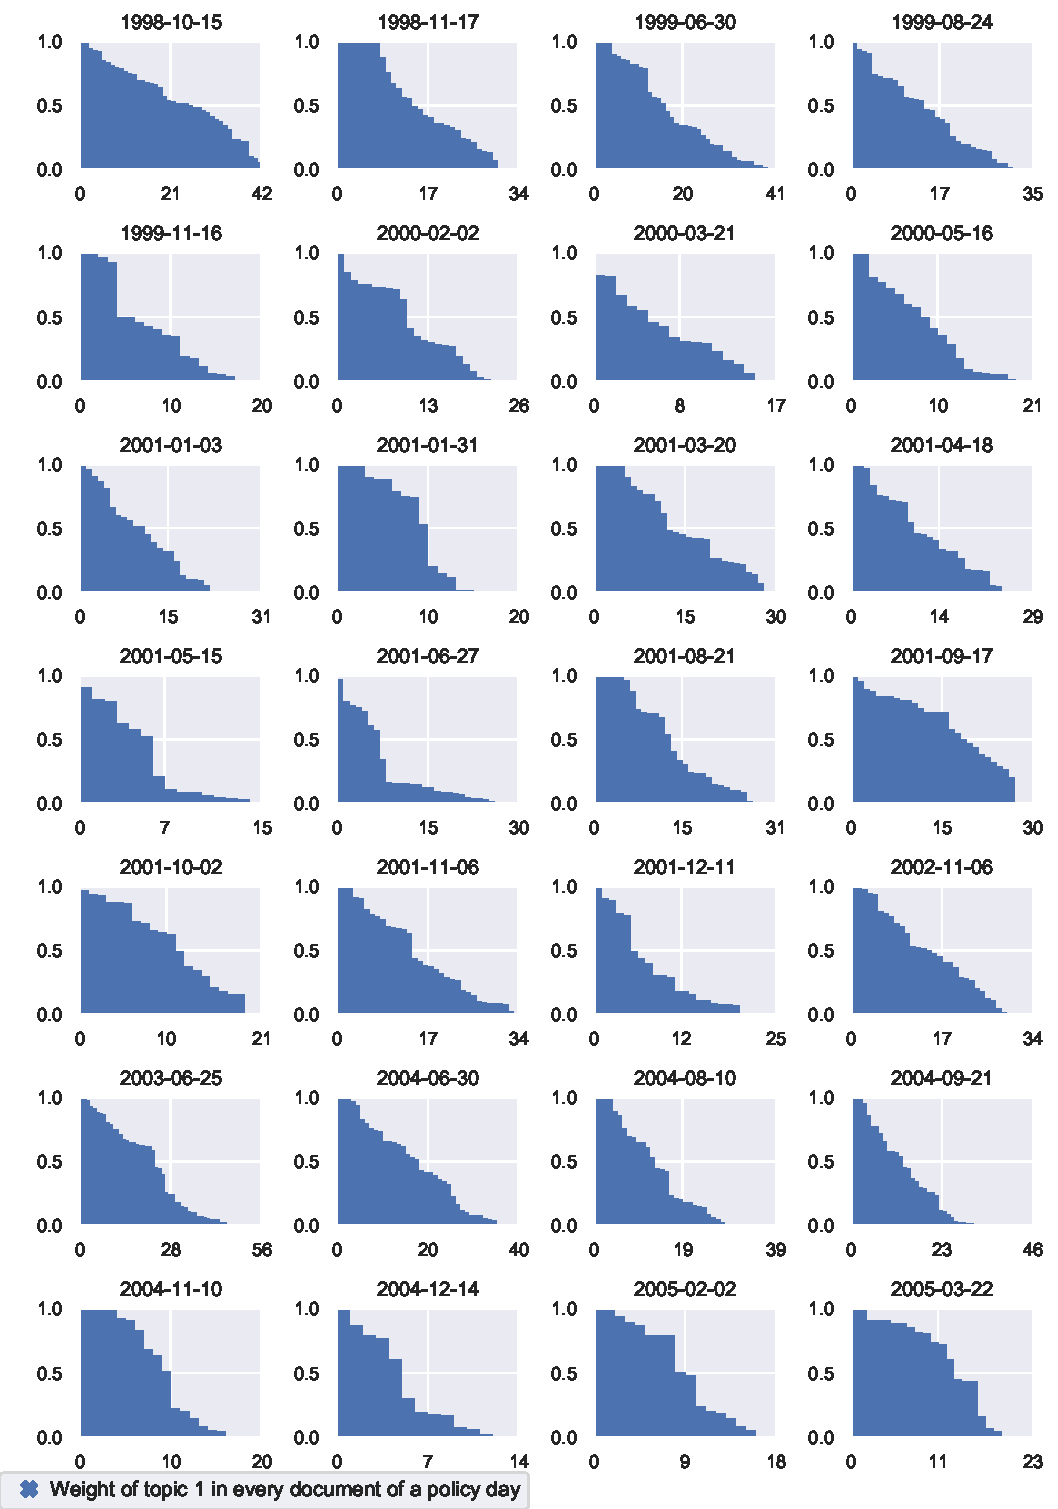
\includegraphics[scale=0.8]{Images/docsplit01_orig.pdf}
	\label{classdoc01}
\end{figure}

\begin{figure}
	\caption{Document classification according to original PLSA - Part II.}
	\centering
	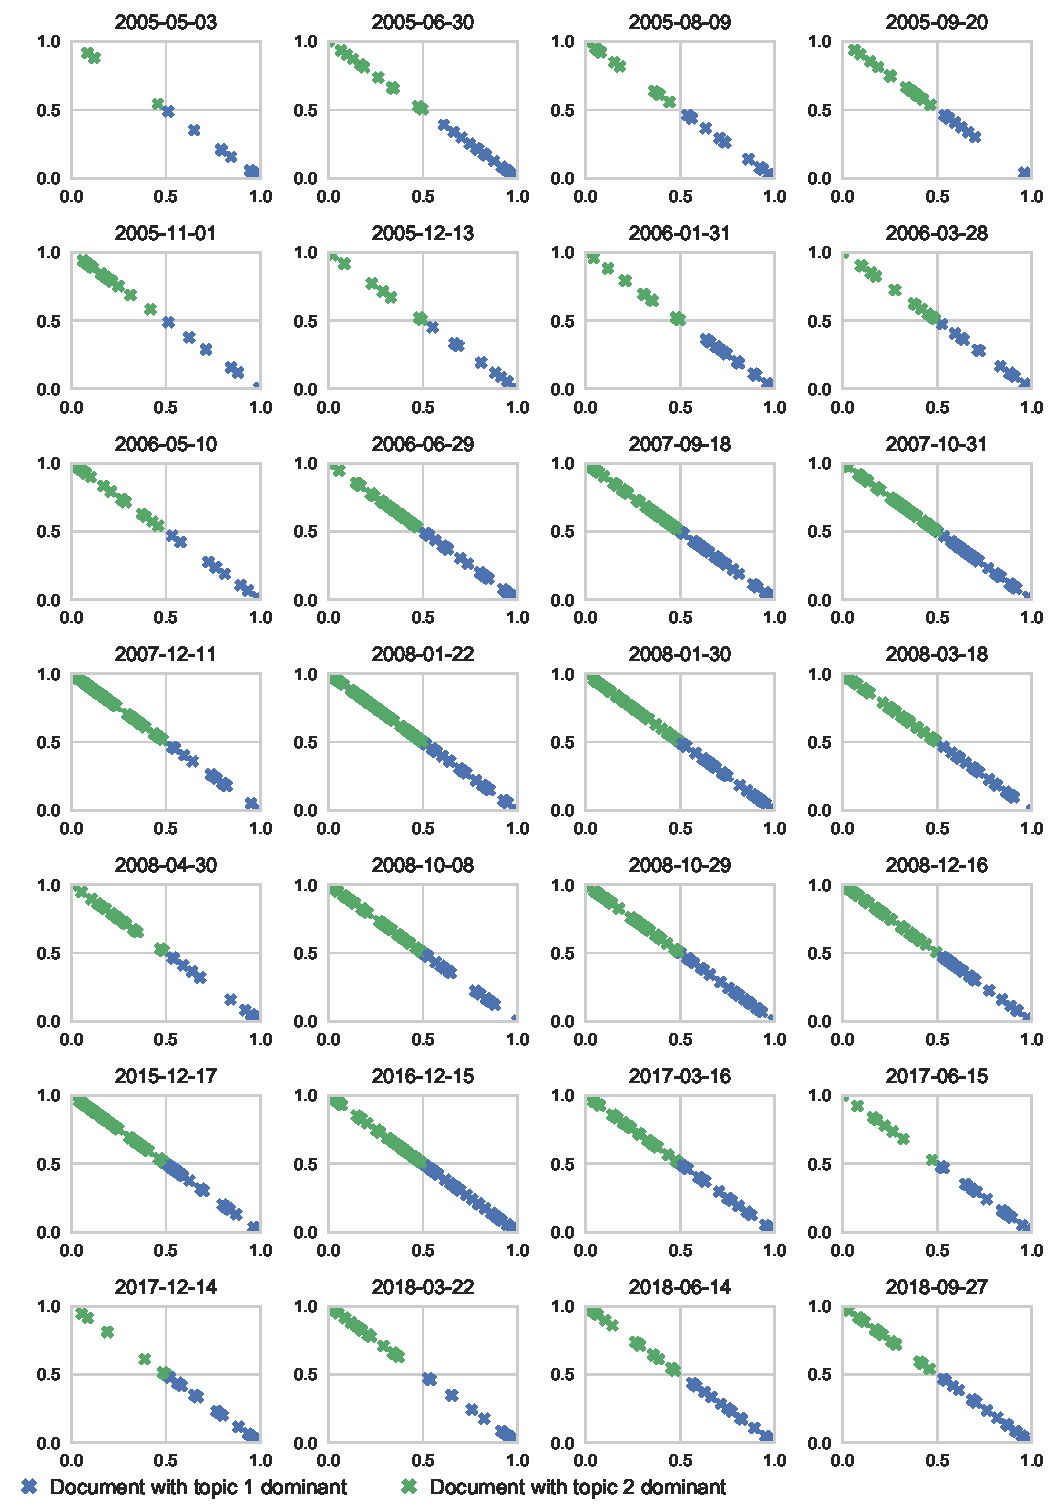
\includegraphics[scale=0.8]{Images/docsplit02_orig.pdf}
	\label{classdoc02}
\end{figure}

%\begin{table}[h] % Add the following just after the closing bracket on this line to specify a position for the table on the page: [h], [t], [b] or [p] - these mean: here, top, bottom and on a separate page, respectively
%	\centering % Centres the table on the page, comment out to left-justify
%	\begin{tabular}{ p{1.5cm}  p{1.5cm}  p{1.5cm}  p{1.5cm}  p{1.5cm}  p{1.5cm}  p{1.5cm}  p{1.5cm}} % The final bracket specifies the number of columns in the table along with left and right borders which are specified using vertical pipes (|); each column can be left, right or center-justified using l, r or c. Columns will widen to hold the content in them by default, to specify a precise width, use p{width}, e.g. p{5cm}
%		\toprule % Top horizontal line
%		\multicolumn{4}{ c }{$\lambda_B=0.8$} & \multicolumn{4}{ c }{$\lambda_B=0.9$} \\
%		
%		\multicolumn{2}{ c }{Topic 1} & \multicolumn{2}{ c }{Topic 2} & \multicolumn{2}{ c }{Topic 1} & \multicolumn{2}{ c }{Topic 2}\\
%		\midrule % In-table horizontal line
%		word & prob & word & prob & word & prob & word & prob\\
%		\midrule
%		 &  &  & &fed&&&\\
%		 &  &  & &inflation&&&\\
%		 &  &  & &&&& \\
%		 &  &  & &&&&\\
%		 &  &  & &&&&\\
%		 &  & & &&&&\\
%		 &  &  &&&&&\\
%		 &  &  &&&&&\\
%		 &  &  &&&&&\\
%		 &  &  &&&&&\\
%		\bottomrule % Bottom horizontal line
%	\end{tabular}
%	\caption{Topics produced by PLSA depending on $\lambda_B$.} % Table caption, can be commented out if no caption is required
%	\label{tab:topics} % A label for referencing this table elsewhere, references are used in text as \ref{label}
%\end{table}

%\begin{table} % Add the following just after the closing bracket on this line to specify a position for the table on the page: [h], [t], [b] or [p] - these mean: here, top, bottom and on a separate page, respectively
%	\centering % Centres the table on the page, comment out to left-justify
%	\begin{tabular}{ p{2cm}  p{2cm}  p{2cm}  p{2cm}  p{2cm}  p{2cm}} % The final bracket specifies the number of columns in the table along with left and right borders which are specified using vertical pipes (|); each column can be left, right or center-justified using l, r or c. Columns will widen to hold the content in them by default, to specify a precise width, use p{width}, e.g. p{5cm}
%		\toprule % Top horizontal line
%		\multicolumn{2}{ c }{$\lambda_B=0.1$}&\multicolumn{2}{ c }{$\lambda_B=0.2$} & \multicolumn{2}{ c }{$\lambda_B=0.3$} \\
%		\midrule
%		Topic 1 & Topic 2 &	Topic 1 & Topic 2 & Topic 1 & Topic 2\\
%		\midrule % In-table horizontal line
%		rate&fed&fed&rate&fed&rate\\
%		year&rate&rate&year&rate&year\\
%		percent&said&said&percent&said&percent\\
%		said&rates&rates&said&rates&said\\
%		bank&inflation&inflation&rates&inflation&rates\\
%		market&economy&economy&interest&economy&bank\\
%		interest&interest&interest&bank&federal&interest\\
%		rates&federal&federal&market&interest&market\\
%		dollar&percent&percent&dollar&economic&cut\\
%		cut&year&economic&cut&policy&dollar\\
%		
%		
%		\toprule % Top horizontal line
%		 \multicolumn{2}{ c }{$\lambda_B=0.4$}&\multicolumn{2}{ c }{$\lambda_B=0.5$} & \multicolumn{2}{ c }{$\lambda_B=0.6$} \\
%		\midrule
%		 Topic 1 & Topic 2 &	Topic 1 & Topic 2 & Topic 1 & Topic 2\\
%		\midrule % In-table horizontal line
%		  fed&rate&fed&rate&fed&year\\
%		  rate&year&rate&year&rate&percent\\
%		  said&percent&said&percent&inflation&rate\\
%		  inflation&said&inflation&bank&economy&bank\\
%		  rates&bank&economy&said&said&market\\
%		  economy&rates&rates&market&rates&dollar\\
%		  federal&interest&federal&interest&economic&interest\\
%		  economic&market&economic&rates&federal&said\\
%		  interest&cut&policy&dollar&policy&rates\\
%		  policy&dollar&interest&investors&growth&investors\\
%		  
%		\toprule
%	\multicolumn{2}{ c }{$\lambda_B=0.7$}&\multicolumn{2}{ c }{$\lambda_B=0.8$} & \multicolumn{2}{ c }{$\lambda_B=0.9$} \\
%		\midrule
%	  Topic 1 & Topic 2 &	Topic 1 & Topic 2 & Topic 1 & Topic 2\\
%		\midrule % In-table horizontal line
%		  fed& year&fed & year&fed&dollar\\
%		  rate& percent&inflation&percent&inflation&per\\
%		  inflation& dollar&rate&dollar&economy& yield\\
%		  economy& rate&economy&bank&economic&cent\\
%		  said& bank&economic&investors&growth &investors\\
%		 rates& market&said&per&policy&rose\\
%		  economic&interest&growth&market&officials&fell\\
%		  growth&investors&rates&yield&greenspan&euro\\
%		 policy&cut&policy&points&would&points\\
%		  federal&per&would&cent&think&trading\\
%		\bottomrule % Bottom horizontal line
%	\end{tabular}
%	\caption{Topics produced by PLSA depending on $\lambda_B$.} % Table caption, can be commented out if no caption is required
%	\label{tab:topics} % A label for referencing this table elsewhere, references are used in text as \ref{label}
%\end{table}
 
 \section{PLSA with background topic}
 
\begin{sidewaystable} % Add the following just after the closing bracket on this line to specify a position for the table on the page: [h], [t], [b] or [p] - these mean: here, top, bottom and on a separate page, respectively
	\centering % Centres the table on the page, comment out to left-justify
	\begin{tabular}{ p{3cm}  p{3cm}  p{3cm}  p{3cm}  p{3cm}  p{3cm}} % The final bracket specifies the number of columns in the table along with left and right borders which are specified using vertical pipes 
		\toprule
	\multicolumn{6}{ c }{Topic 1} \\
		\midrule
	  $\lambda_B=0.1$ & $\lambda_B=0.2$ &	$\lambda_B=0.3$ & $\lambda_B=0.4$ & $\lambda_B=0.5$ & $\lambda_B=0.6$ \\
		\midrule % In-table horizontal line
		 \textcolor{gray}{said}  		& \textcolor{gray}{year} 			& \textcolor{gray}{year}  		& \textcolor{gray}{year }			& \textcolor{gray}{year }		& \textcolor{gray}{year} \\
		 \textcolor{gray}{year }  		& \textcolor{gray}{said }			& \textcolor{gray}{said }		& \textcolor{gray}{percent }		& \textcolor{gray}{percent }	& \textcolor{gray}{percent} \\
		 \textcolor{gray}{percent}  	& \textcolor{gray}{percent }		& \textcolor{gray}{percent }	& \textcolor{gray}{said} 			& \textcolor{gray}{said} 		& \textcolor{gray}{market }\\
		 \textcolor{gray}{market}  		& \textcolor{gray}{market} 			& \textcolor{gray}{market} 		& \textcolor{gray}{market} 			&\textcolor{gray}{market} 		& \textcolor{purple}{dollar} \\
		 \textcolor{gray}{rate}   		& \textcolor{gray}{rate }			& \textcolor{purple}{dollar}	& \textcolor{purple}{dollar}		&\textcolor{purple}{dollar}		& \textcolor{gray}{said} \\
		 \textcolor{purple}{dollar}		& \textcolor{purple}{dollar}		& \textcolor{gray}{rate}		& \textcolor{gray}{rate}			&\textcolor{gray}{bank  }		& \textcolor{gray}{bank  } \\
		 cut  							& cut 								& \textcolor{gray}{bank  }		& \textcolor{gray}{bank  }			&\textcolor{red}{investors}		& \textcolor{red}{investors} \\
		 \textcolor{gray}{bank  }		& \textcolor{gray}{bank  }			& cut 							& cut 								&cut 							& cut \\
		 \textcolor{gray}{rates}		& \textcolor{red}{investors}		& \textcolor{red}{investors}	& \textcolor{red}{investors}		&\textcolor{gray}{rate}			& \textcolor{gray}{rate} \\
		 \textcolor{red}{investors}		& \textcolor{gray}{rates}			& \textcolor{gray}{rates}		& \textcolor{gray}{rates}			&\textcolor{gray}{rates}		& per cent\\
		 fed  							& interest rate 					& interest rate					& interest rate						&per cent						& \textcolor{magenta}{yield} \\
		 interest  rate					& fed 								& per cent						& per cent							&interest rate					& bond \\
		 per cent 						& per cent 							& bond 							& bond 								&bond 							& interest rate\\
		 \textcolor{gray}{federal reserve }& bond 							& \textcolor{magenta}{yield}	& \textcolor{magenta}{yield}		&\textcolor{magenta}{yield}		& \textcolor{gray}{rates} \\
		 bond  							& \textcolor{gray}{federal reserve }& markets 						& \textcolor{orange}{rose }			&\textcolor{orange}{rose }		& \textcolor{orange}{rose }	 \\
		 markets  						& \textcolor{magenta}{yield}		& \textcolor{gray}{federal reserve }& markets 							&\textcolor{cyan}{index }		& \textcolor{cyan}{index } \\
		 \textcolor{magenta}{yield}		& markets 							& \textcolor{orange}{rose }		& \textcolor{cyan}{index }			&markets 						& \textcolor{violet}{fell } \\
		 expected  						& \textcolor{orange}{rose }			& expected 						& \textcolor{gray}{federal reserve }&\textcolor{violet}{fell }		& markets \\
		 interest rate 					& expected							& \textcolor{cyan}{index }		& expected 							&month 							& \textcolor{green}{stocks} \\
		 \textcolor{orange}{rose}  		& \textcolor{cyan}{index }			& us 							& \textcolor{violet}{fell }			&expected 						& month \\		  
		\bottomrule % Bottom horizontal line
	\end{tabular}
	\caption{Topic 1 produced by PLSA depending on $\lambda_B$.} % Table caption, can be commented out if no caption is required
	\label{tab:topics} % A label for referencing this table elsewhere, references are used in text as \ref{label}
\end{sidewaystable}

\begin{sidewaystable} % Add the following just after the closing bracket on this line to specify a position for the table on the page: [h], [t], [b] or [p] - these mean: here, top, bottom and on a separate page, respectively
	\centering % Centres the table on the page, comment out to left-justify
	\begin{tabular}{ p{3cm}  p{3cm}  p{3cm} | p{3cm}  p{3cm}  p{3cm}} % The final bracket specifies the number of columns in the table along with left and right borders which are specified using vertical pipes 
		\toprule
		\multicolumn{3}{ c |}{Topic 1} &  \multicolumn{3}{ c }{Topic 2}\\
		\midrule
		$\lambda_B=0.7$ & $\lambda_B=0.8$ &	$\lambda_B=0.9$ &  $\lambda_B=0.1$ & $\lambda_B=0.2$ & $\lambda_B=0.3$ \\
		\midrule % In-table horizontal line
		  \textcolor{gray}{year }				& \textcolor{purple}{dollar}	&\textcolor{purple}{dollar}		& 	\textcolor{gray}{fed} 				& \textcolor{gray}{fed} 		& \textcolor{gray}{fed} \\
		  \textcolor{gray}{percent }			&\textcolor{gray}{year }		&\textcolor{red}{investors}		& 	\textcolor{gray}{said} 				& \textcolor{gray}{said} 		& \textcolor{gray}{said} \\
		  \textcolor{purple}{dollar}			&\textcolor{gray}{percent} 		&\textcolor{magenta}{yield}		& 	\textcolor{gray}{inflation} 		&\textcolor{gray}{inflation} 	& \textcolor{gray}{inflation} \\
		  \textcolor{gray}{market  }		 	&\textcolor{gray}{market }		&\textcolor{gray}{bank  }		& 	\textcolor{gray}{economy} 			&\textcolor{gray}{economy} 		& \textcolor{gray}{economy} \\
		  \textcolor{gray}{bank  }				&\textcolor{red}{investors}		&\textcolor{orange}{rose }		& 	\textcolor{gray}{rate} 				&\textcolor{gray}{rate}			& \textcolor{gray}{rate} \\
		  \textcolor{red}{investors}			&\textcolor{gray}{bank  }		&per cent						& 	\textcolor{gray}{would} 			&\textcolor{gray}{would} 		& \textcolor{gray}{would} \\
		  cut  									&\textcolor{magenta}{yield}		&\textcolor{violet}{fell }		& 	\textcolor{gray}{year}				&\textcolor{magenta}{economic}	& \textcolor{magenta}{economic} \\
		  \textcolor{gray}{said}  			 	&\textcolor{orange}{rose }		&\textcolor{blue}{trading}		& 	\textcolor{magenta}{economic}		&\textcolor{gray}{rates}		& \textcolor{gray}{rates} \\
		  \textcolor{magenta}{yield}			&per cent						&\textcolor{gray}{year} 		& 	\textcolor{gray}{rates}				&\textcolor{gray}{year}			& \textcolor{blue}{growth} \\
		  per cent		  						&cut 							&bond 							& 	\textcolor{blue}{growth }			&\textcolor{blue}{growth}		& \textcolor{gray}{year}\\
		  \textcolor{orange}{rose }				&bond 							&\textcolor{cyan}{index }		& 	policy 								&policy			 				& policy \\
		  bond 			  						&\textcolor{violet}{fell }		&\textcolor{green}{stocks}		& 	percent 							&percent 						& could \\
		  \textcolor{cyan}{index }				&\textcolor{cyan}{index }		&yen 							& 	\textcolor{gray}{federal reserve}	&\textcolor{gray}{interest rates}& \textcolor{gray}{interest rates}\\
		  \textcolor{violet}{fell } 		 	&\textcolor{green}{stocks}		&euro 							& 	\textcolor{gray}{interest rates}	&could 							& percent \\
		  interest rate  						&\textcolor{blue}{trading}		&currency 						& 	could 								&\textcolor{gray}{federal reserve}& \textcolor{gray}{federal reserve}\\
		  \textcolor{green}{stocks}				&month 							&bonds 							& 	market 								&market 						& meeting \\
		  \textcolor{gray}{rate  }				&bonds 							&shares 						& 	meeting 							&meeting 						& \textcolor{cyan}{statement} \\
		  month 		  						&euro 							&cents 							& \textcolor{cyan}{statement}			&\textcolor{cyan}{statement}	& market \\
		  \textcolor{gray}{rates}				&new york						&bps 							& 	time 								&time 							& time \\
		  \textcolor{blue}{trading}				&basis points					&china 							& 	\textcolor{gray}{interest rate}		&\textcolor{gray}{interest rate}&one  \\		  
		\bottomrule % Bottom horizontal line
	\end{tabular}
	\caption{Topic 1 and Topic 2 produced by PLSA depending on $\lambda_B$.} % Table caption, can be commented out if no caption is required
	\label{tab:topics2} % A label for referencing this table elsewhere, references are used in text as \ref{label}
\end{sidewaystable}


\begin{sidewaystable} % Add the following just after the closing bracket on this line to specify a position for the table on the page: [h], [t], [b] or [p] - these mean: here, top, bottom and on a separate page, respectively
	\centering % Centres the table on the page, comment out to left-justify
	\begin{tabular}{ p{3cm}  p{3cm}  p{3cm}  p{3cm}  p{3cm}  p{3cm}} % The final bracket specifies the number of columns in the table along with left and right borders which are specified using vertical pipes 
		\toprule
		\multicolumn{6}{ c }{Topic 2} \\
		\midrule
		$\lambda_B=0.4$ & $\lambda_B=0.5$ &	$\lambda_B=0.6$ & $\lambda_B=0.7$ & $\lambda_B=0.8$ & $\lambda_B=0.9$  \\
		\midrule % In-table horizontal line
		\textcolor{gray}{fed} 			&\textcolor{gray}{fed } 			&\textcolor{gray}{fed  }			& \textcolor{gray}{fed}  			&\textcolor{gray}{fed }			& \textcolor{gray}{fed} \\
		\textcolor{gray}{said} 			&\textcolor{gray}{said}  			& \textcolor{gray}{inflation} 		& \textcolor{gray}{inflation}  		&\textcolor{gray}{inflation} 	&\textcolor{gray}{inflation}  \\
		\textcolor{gray}{inflation} 	&\textcolor{gray}{inflation} 		& \textcolor{gray}{economy} 		& \textcolor{gray}{economy } 		&\textcolor{gray}{economy}		& \textcolor{gray}{economy} \\
		\textcolor{gray}{economy} 		&\textcolor{gray}{economy}  		& \textcolor{gray}{said} 			& \textcolor{gray}{said } 			&\textcolor{gray}{said} 		& \textcolor{magenta}{economic} \\
		\textcolor{gray}{rate} 			& \textcolor{gray}{rate} 			& \textcolor{gray}{rate} 			& \textcolor{gray}{would} 			&\textcolor{magenta}{economic}	& \textcolor{blue}{growth}\\
		\textcolor{gray}{would} 		& \textcolor{gray}{would} 			& \textcolor{gray}{would} 			& \textcolor{gray}{rate }			&\textcolor{gray}{would }		& \textcolor{green}{greenspan} \\
		\textcolor{magenta}{economic}	& \textcolor{magenta}{economic}		& \textcolor{magenta}{economic}		& \textcolor{magenta}{economic}		&\textcolor{blue}{growth}		& \textcolor{gray}{would} \\
		\textcolor{blue}{growth}		& \textcolor{blue}{growth}			& \textcolor{blue}{growth}			& \textcolor{blue}{growth}			&\textcolor{gray}{rate} 		& think \\
		\textcolor{gray}{rates} 		& policy 							& policy 							& policy 							&policy 						& policy \\
		policy 							& \textcolor{gray}{rates} 			& \textcolor{gray}{rates} 			& could 							& \textcolor{green}{greenspan}	& \textcolor{olive}{bernanke} \\
		\textcolor{gray}{year}			& could 							& could 							& \textcolor{gray}{rates} 			&\textcolor{cyan}{statement}	& \textcolor{cyan}{statement} \\
		could 							& meeting 							& meeting 							& meeting 							&meeting 						& \textcolor{teal}{chairman} \\
		\textcolor{gray}{interest rates}& \textcolor{gray}{interest rates}	& \textcolor{cyan}{statement}		& \textcolor{cyan}{statement}		&think 							& mr \\
		\textcolor{gray}{federal reserve}& \textcolor{cyan}{statement}		& \textcolor{gray}{interest rates}	& time 								&could 							& meeting \\
		meeting 						& \textcolor{gray}{federal reserve}	& time 								& think 							&mr 							& \textcolor{violet}{economists} \\
		\textcolor{cyan}{statement}		& time 								& \textcolor{gray}{federal reserve}	& mr 								&time 							& spending \\
		percent 						& \textcolor{gray}{year}			& mr   								& \textcolor{gray}{interest rates}	&\textcolor{olive}{bernanke}& fomc \\
		time 							& mr 								& think   							& \textcolor{green}{greenspan}		&\textcolor{teal}{chairman} 	& washington \\
		market 							& one 								& one  								& \textcolor{gray}{federal reserve}	&\textcolor{violet}{economists}	& consumer \\
		one 							& think 							& \textcolor{green}{greenspan} 		& one 								&\textcolor{gray}{rates  }		& know \\		  
		\bottomrule % Bottom horizontal line
	\end{tabular}
	\caption{Topic 2 produced by PLSA depending on $\lambda_B$.} % Table caption, can be commented out if no caption is required
	\label{tab:topics3} % A label for referencing this table elsewhere, references are used in text as \ref{label}
\end{sidewaystable}

\begin{sidewaysfigure}
	\caption{Policy day classification according to PLSA with $\lambda_B = 0.1$.}
	\centering
	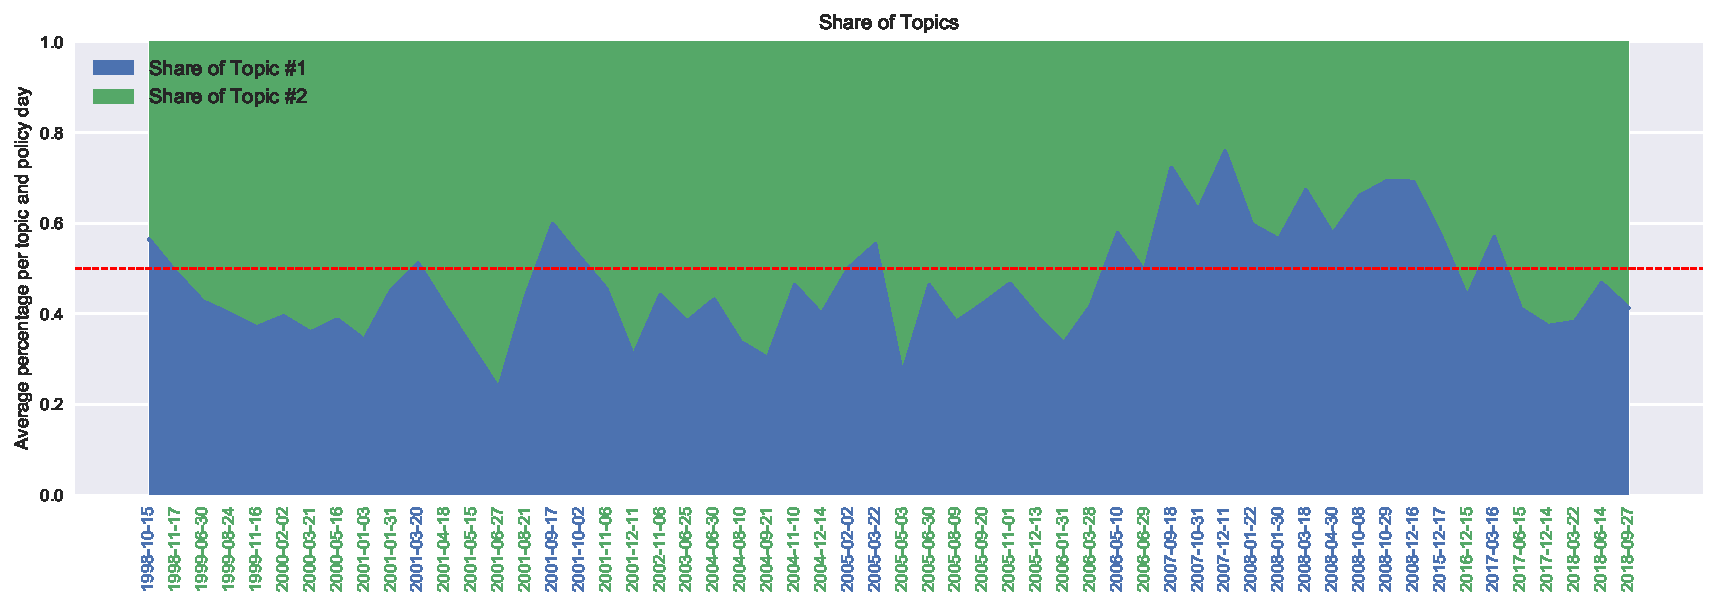
\includegraphics[scale=0.8]{Images/plsamodelling_bgLamb_0_1.pdf}
	\label{classPLSAL01}
\end{sidewaysfigure}

\begin{figure}
	\caption{Document classification according to PLSA with $\lambda_B = 0.1$ - Part I.}
	\centering
	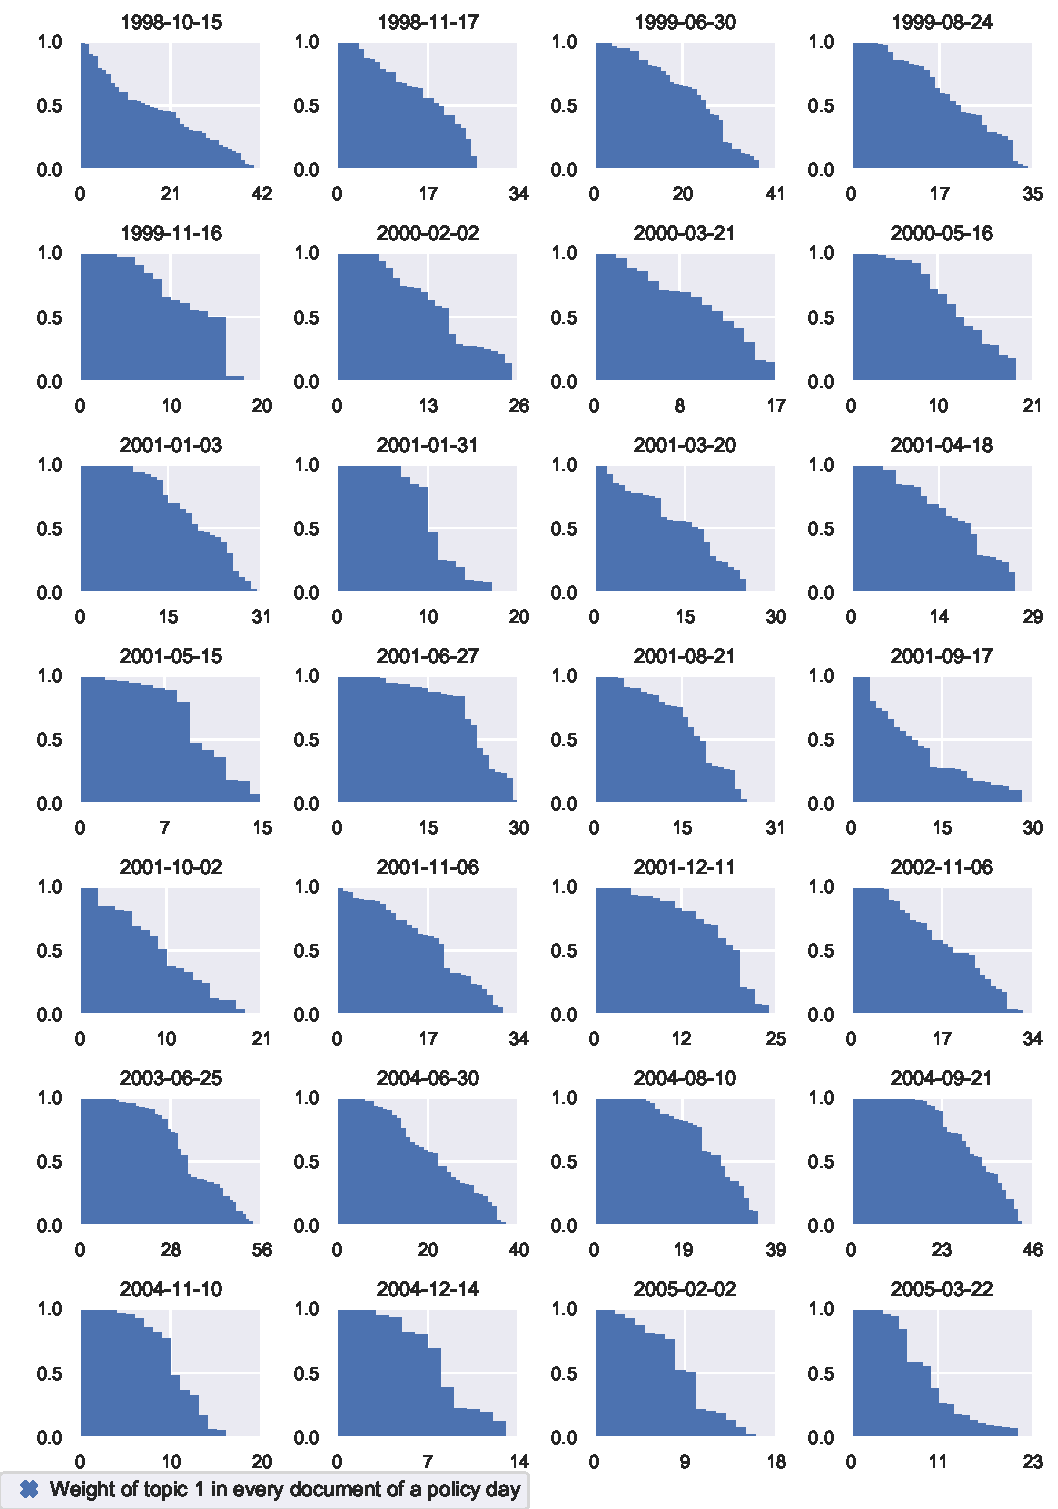
\includegraphics[scale=0.8]{Images/docsplit01_bgLamb_0_1.pdf}
	\label{classdoc01L01}
\end{figure}

\begin{figure}
	\caption{Document classification according to PLSA with $\lambda_B = 0.1$ - Part II.}
	\centering
	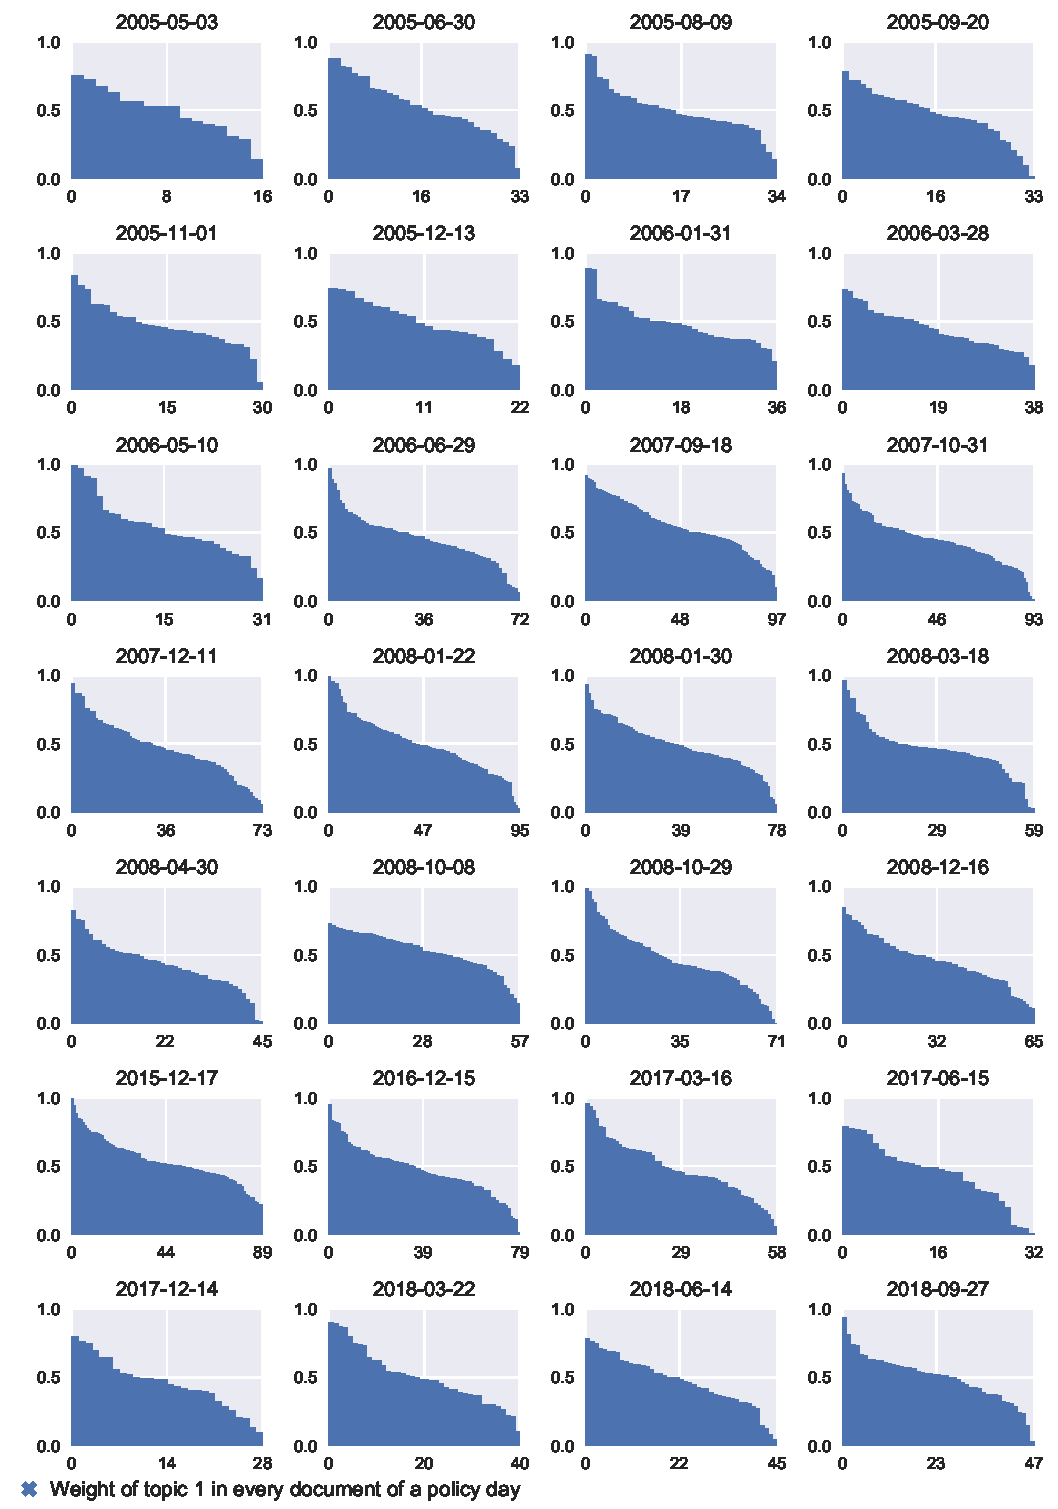
\includegraphics[scale=0.8]{Images/docsplit02_bgLamb_0_1.pdf}
	\label{classdoc02L01}
\end{figure}

\begin{sidewaysfigure}
	\caption{Policy day classification according to PLSA with $\lambda_B = 0.9$.}
	\centering
	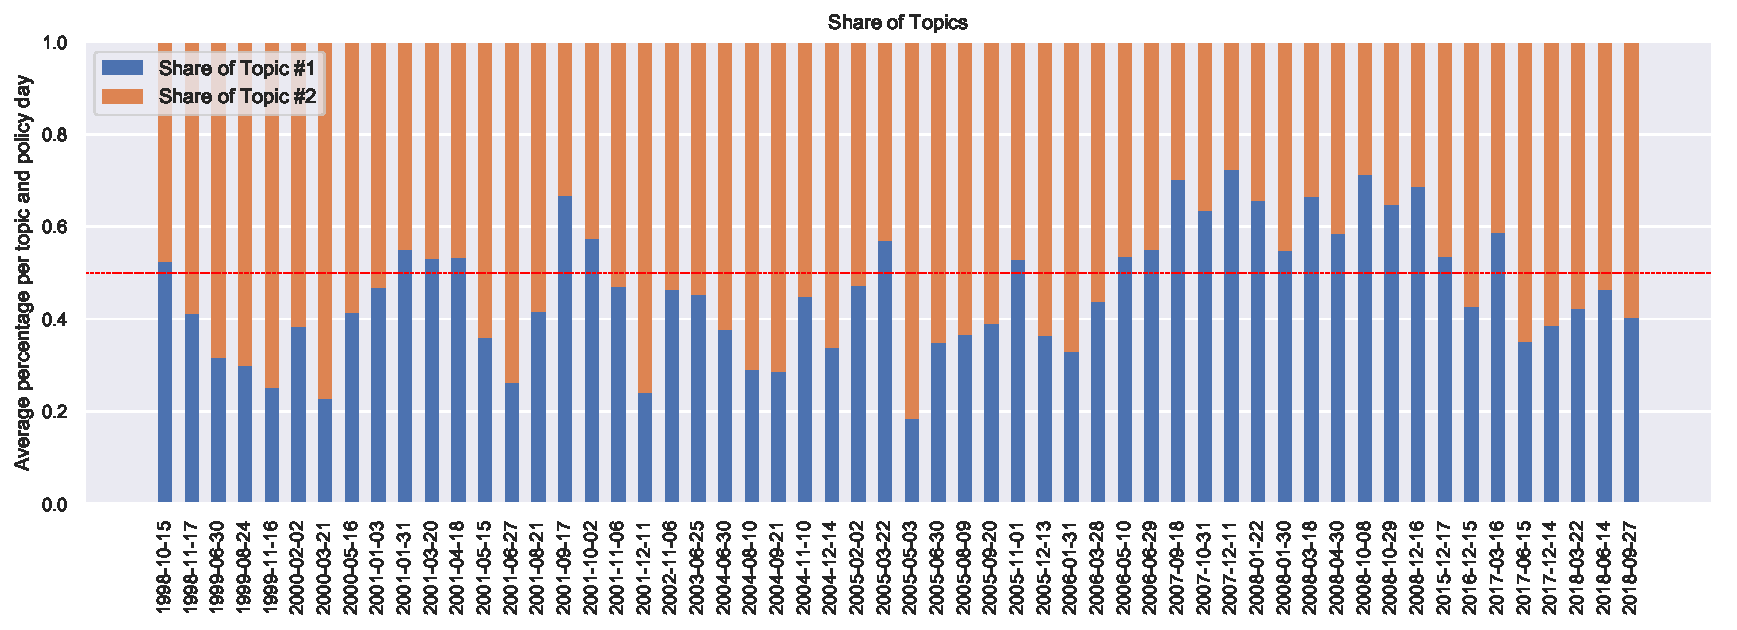
\includegraphics[scale=0.8]{Images/plsamodelling_bgLamb_0_9.pdf}
	\label{classPLSAL09}
\end{sidewaysfigure}

\begin{figure}
	\caption{Document classification according to PLSA with $\lambda_B = 0.9$ - Part I.}
	\centering
	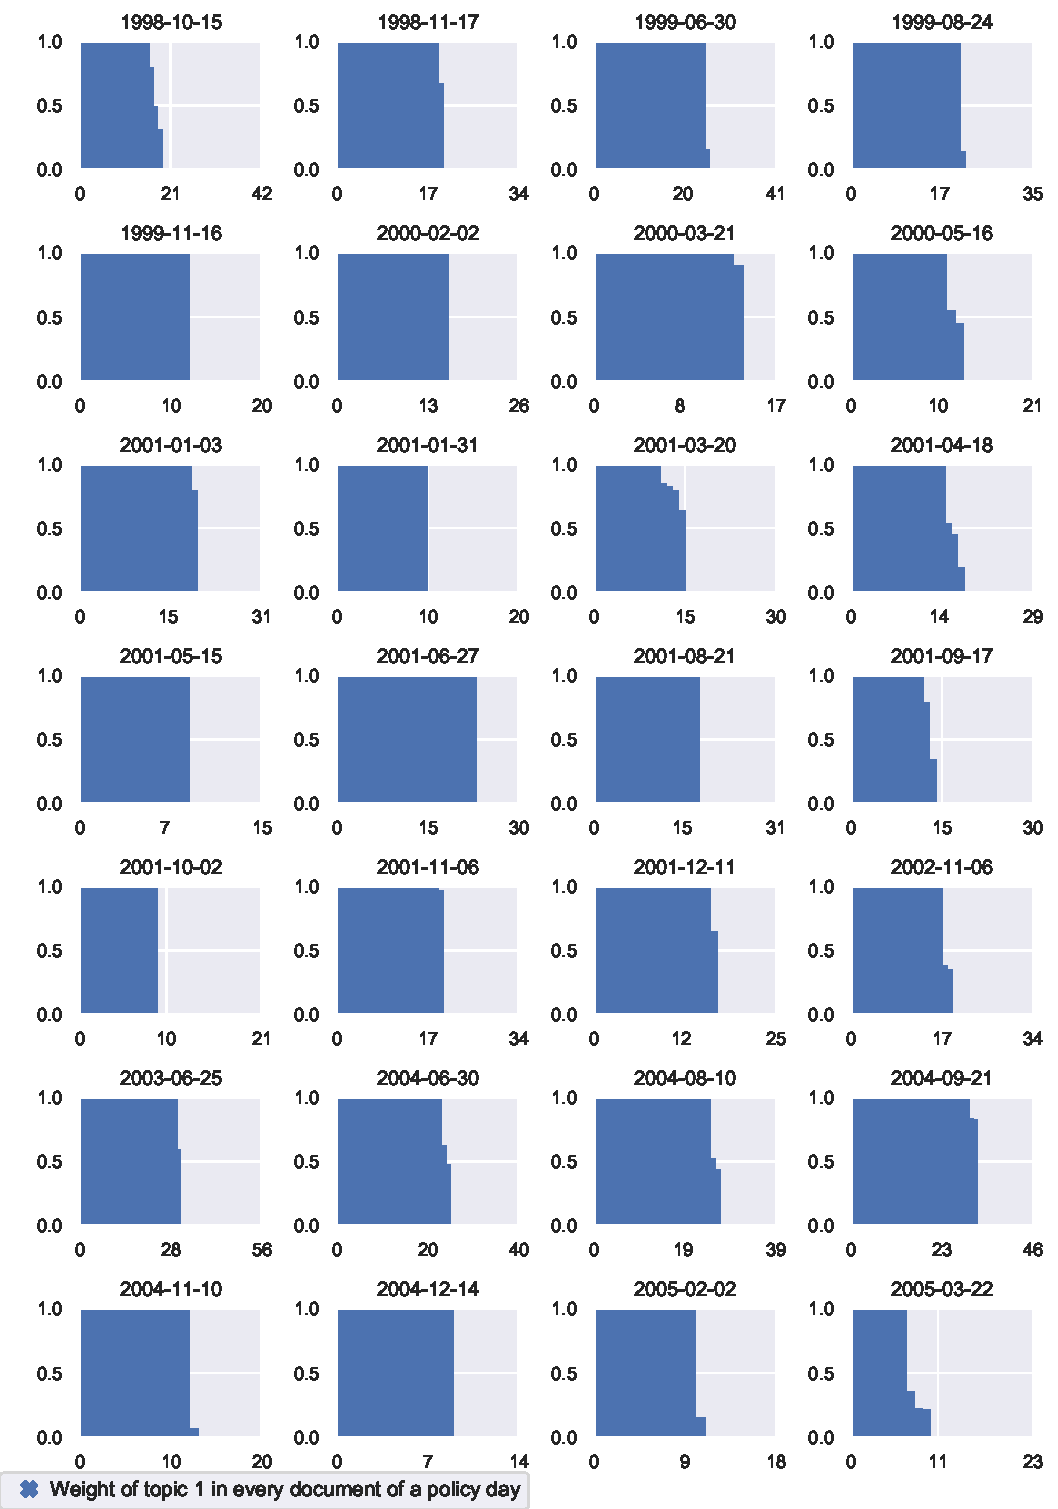
\includegraphics[scale=0.8]{Images/docsplit01_bgLamb_0_9.pdf}
	\label{classdoc01L09}
\end{figure}

\begin{figure}
	\caption{Document classification according to PLSA with $\lambda_B = 0.9$ - Part II.}
	\centering
	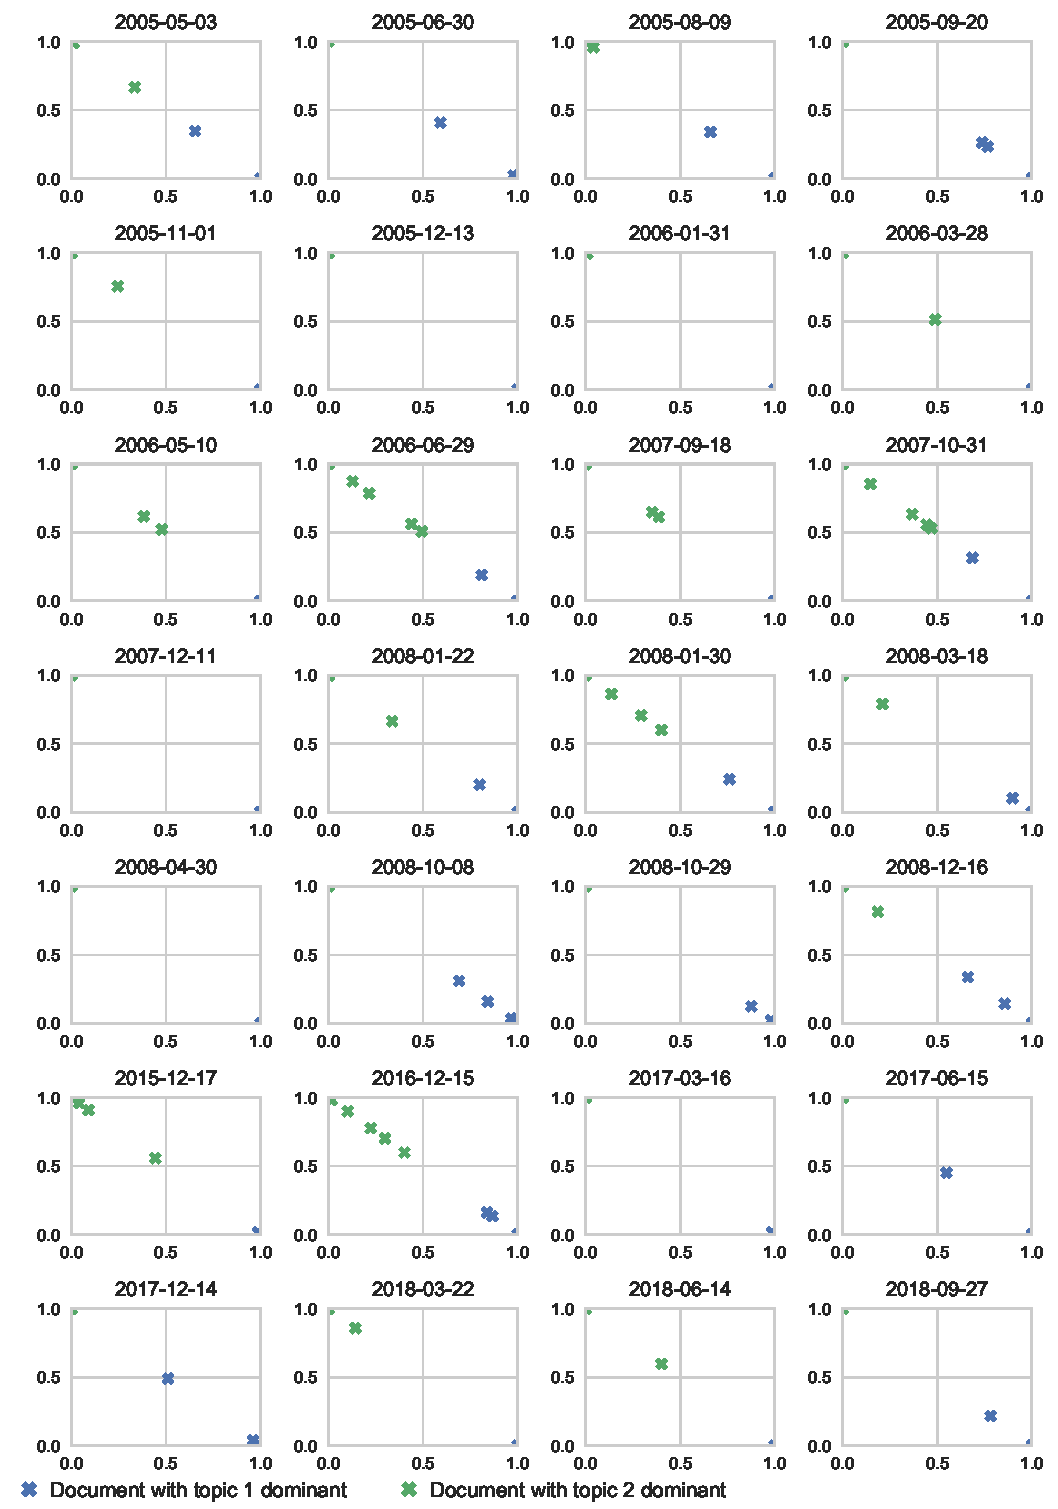
\includegraphics[scale=0.8]{Images/docsplit02_bgLamb_0_9.pdf}
	\label{classdoc02L09}
\end{figure}

\renewcommand{\theequation}{D.\arabic{equation}}


\chapter{Classification and Regression Results}\label{AppendixD}

\begin{figure}
	\caption{Response of the 10-year interest rate to a change in the 3-month rate on policy days influenced by Narrative one ($\lambda_B=0.1$).}
	\centering
	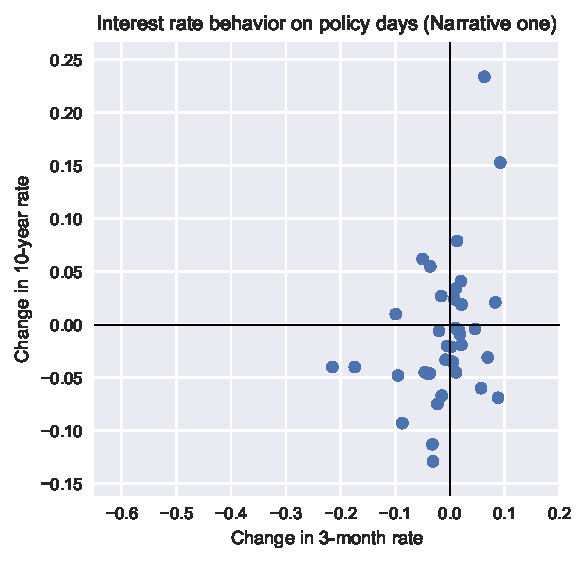
\includegraphics[scale=1]{Images/ChangePlot02_L0_1.pdf}
	\label{Change02_L01}
\end{figure}

\begin{figure}
	\caption{Response of the 10-year interest rate to a change in the 3-month rate on policy days influenced by Narrative two ($\lambda_B=0.1$).}
	\centering
	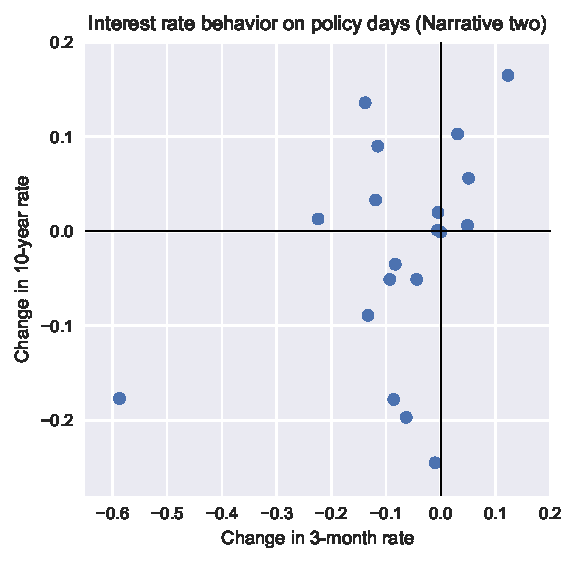
\includegraphics[scale=1]{Images/ChangePlot03_L0_1.pdf}
	\label{Change03_L01}
\end{figure}

\begin{figure}
	\caption{Response of the 10-year interest rate to a change in the 3-month rate on policy days influenced by Narrative one ($\lambda_B=0.9$).}
	\centering
	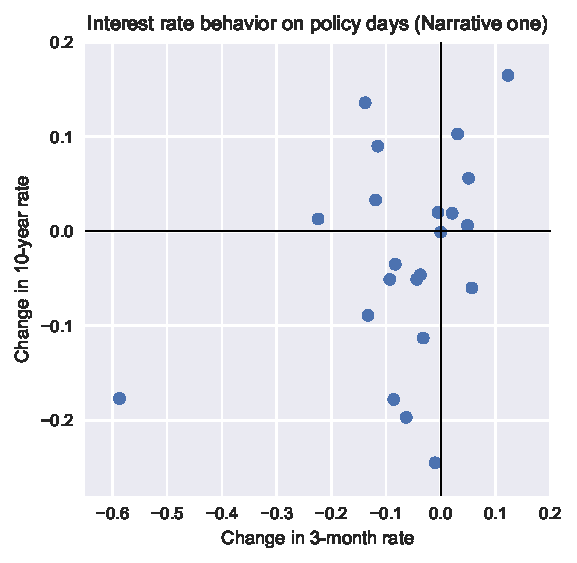
\includegraphics[scale=1]{Images/ChangePlot02_L0_9.pdf}
	\label{Change02_L09}
\end{figure}

\begin{figure}
	\caption{Response of the 10-year interest rate to a change in the 3-month rate on policy days influenced by Narrative two ($\lambda_B=0.9$).}
	\centering
	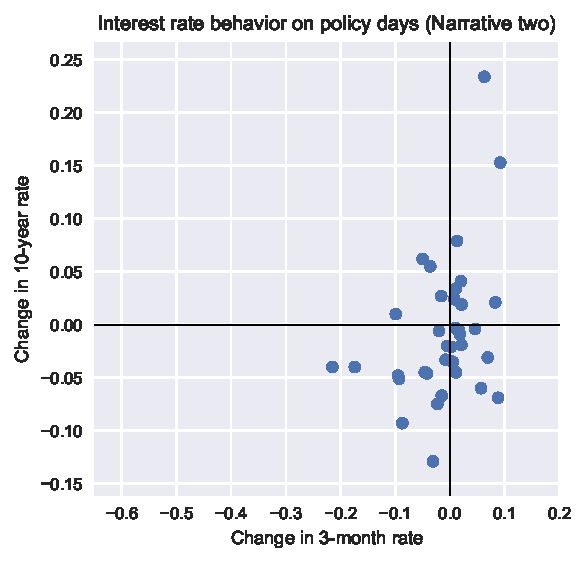
\includegraphics[scale=1]{Images/ChangePlot03_L0_9.pdf}
	\label{Change03_L09}
\end{figure}


\section{For Example... }

\lipsum[2-8]

\newpage
{\pagestyle{firststyle}
	
\chapter*{Declaration of Authorship}

"I hereby declare
\begin{itemize}
	\item that I have written this thesis without any help from others and without the use of
	documents and aids other than those stated above;
	\item that I have mentioned all the sources used and that I have cited them correctly
	according to established academic citation rules;
	\item that I have acquired any immaterial rights to materials I may have used such as images
	or graphs, or that I have produced such materials myself;
	\item that the topic or parts of it are not already the object of any work or examination of
	another course unless this has been explicitly agreed on with the faculty member in
	advance and is referred to in the thesis;
	\item that I will not pass on copies of this work to third parties or publish them without the
	University’s written consent if a direct connection can be established with the
	University of St.Gallen or its faculty members;
	\item that I am aware that my work can be electronically checked for plagiarism and that I
	hereby grant the University of St.Gallen copyright in accordance with the Examination
	Regulations in so far as this is required for administrative action;
	\item that I am aware that the University will prosecute any infringement of this declaration
	of authorship and, in particular, the employment of a ghostwriter, and that any such
	infringement may result in disciplinary and criminal consequences which may result
	in my expulsion from the University or my being stripped of my degree."
\end{itemize}

%\noindent By submitting this academic term paper, I confirm through my conclusive action that I am
%submitting the Declaration of Authorship, that I have read and understood it, and that it is
%true.

%\hrule
\vspace*{3cm}
%\hrule


\dotbox{Location, Date} \hfill \dotbox{Signature}\\

\vspace*{.5 cm}
\noindent By submitting this academic term paper, I confirm through my conclusive action that I am
submitting the Declaration of Authorship, that I have read and understood it, and that it is
true.
\cleardoublepage
}
\end{document}
